
\documentclass{aitthesis}

% ---------- Additional packages needed for content (formatting itself comes from aitthesis.cls) ----------
\usepackage{amsmath,amssymb}
\usepackage{setspace}
\usepackage{graphicx}
\usepackage{booktabs}
\usepackage{array}
\usepackage{tabularx}
\usepackage{longtable}
\usepackage{float}
\usepackage{subcaption}

\graphicspath{{figures/}}
\hypersetup{hidelinks}
\sloppy

% Tighter float spacing: default report-class gaps around figures left large
% blank gutters once dashboard screenshots were enlarged and stacked.
\setlength{\textfloatsep}{10pt plus 2pt minus 2pt}
\setlength{\floatsep}{8pt plus 2pt minus 2pt}
\setlength{\intextsep}{8pt plus 2pt minus 2pt}
\captionsetup{skip=4pt}

% ---------- Metadata ----------
\newcommand{\reporttitle}{Smart Workout: A RAG-Assisted Decision Support and
Business Intelligence System for Personalized Weight Training}

\newcommand{\studentname}{Aye Khin Khin Hpone (Yolanda Lim)}
\newcommand{\studentid}{st125970}
\newcommand{\studentnameii}{Waranon Neamtuptim (Non)}
\newcommand{\studentidii}{st125934}
\newcommand{\studentnameiii}{Jirapat Datephanyawat (Earth)}
\newcommand{\studentidiii}{st125843}
\newcommand{\degreeprogram}{AT82.04: Business Intelligence and Analytics \\
Intersem 2026}
\newcommand{\submissiondate}{July 2026}


\begin{document}

% ==================== TITLE PAGE ====================
\begin{titlepage}
\thispagestyle{empty}
\singlespacing
\centering

{\bfseries\Large \reporttitle\par}
\vspace{0.45in}

\textit{Final report}

{by\par}
\vspace{0.20in}

{\bfseries
\studentname\_\studentid\par
\studentnameii\_\studentidii\par
\studentnameiii\_\studentidiii\par
}

\vspace{0.42in}

\begin{minipage}{0.82\textwidth}
\centering


\textbf{\degreeprogram}
\end{minipage}
\vspace{0.42in}

Dr. Vatcharaporn Esichaikul\\
TA: Anushka Ojha

\vfill
{Asian Institute of Technology\par}
{Faculty of Advanced Science and Technology (FAST)\par}
{Thailand\par}
{\submissiondate\par}
\end{titlepage}

% ==================== FRONT MATTER ====================
\pagenumbering{roman}
\addtocontents{toc}{~\hfill\textbf{Page}\par}

\phantomsection
\addcontentsline{toc}{chapter}{\bf ABSTRACT}
\begin{center}
    \large{\bf ABSTRACT}
\end{center}


Smart Workout is a Retrieval-Augmented Generation (RAG)-assisted Decision Support and Business Intelligence system for personalized weight-training planning. It integrates gym membership, exercise-tracking, lifestyle, and nutrition data into one descriptive, predictive, and prescriptive workflow, delivered as a React/FastAPI prototype with XGBoost prediction, rule-based readiness logic, RAG-grounded exercise retrieval, and an embedded Tableau map. Executives get branch utilization, revenue, and lifestyle-segment views; individual users get readiness-aware guidance from profile, wellness, goal, and equipment inputs.

Two supervised tasks were evaluated with 5-fold cross-validation, and XGBoost was selected for both. The regressor reached RMSE 15.021 kcal/hr and $R^2=0.970$ for calorie-burn-rate estimation -- reported as a deployment-aware upper bound since its dominant feature, average BPM, is estimated at inference rather than measured. The classifier reached macro-F1 0.342 for three-class workout-intensity prediction; macro-F1 is used instead of accuracy because the classes are imbalanced and the model trails the majority-class baseline on raw accuracy. The result is an explainable dashboard and plan-generation workflow linking engineered data, transparent model results, RAG-grounded recommendations, and business decision mapping.


\vspace{0.5em}
\noindent\textbf{Keywords:} Decision Support System, Business Intelligence, Retrieval-Augmented Generation, XGBoost, Personalized Training, Dashboard Analytics
\clearpage

\tableofcontents
\clearpage

% ==================== MAIN MATTER ====================
\pagenumbering{arabic}

% ==================== CHAPTER 1 ====================
\chapter{INTRODUCTION}
\section{Background of the Study}
Weight training is widely practiced for strength and fitness, yet many gym users struggle to plan effectively: they
are uncertain which exercises suit a given body part, how to adapt to available equipment, how to structure a
weekly timetable, and whether their physical condition supports a particular plan. Most decisions rely on generic
online routines that ignore personal factors -- age, sleep, BMI, physiological indicators, equipment, schedule --
producing a mismatch between plan and readiness. This project proposes Smart Workout, a combined Decision
Support System (DSS) and Business Intelligence System (BIS) (Power, 2002; Chaudhuri et al., 2011) that
unifies multi-source real-world data, a Retrieval-Augmented Generation (RAG) knowledge layer, and supervised
ML models within an interactive web dashboard, transforming user-provided inputs into descriptive insight,
predictive outcome estimates, and prescriptive training plans while preserving human oversight. The primary
target users are gym members seeking personalized training guidance; fitness coaches constitute a secondary
audience using the dashboard for decision-support reference; and gym managers form a third, executive audience
that uses the same dashboard for branch-level utilization, revenue, and segment monitoring.

\section{Objectives of the Study}

The project is expected to deliver a functional DSS/BIS prototype that fulfils the following objectives, explicitly covering the descriptive, predictive, and prescriptive analytics layers required of a BI system:
\begin{itemize}
    \item \textbf{Data collection \& preparation:} clean and standardize multi-source public datasets (gym membership and check-in records, exercise catalogue, gym-member workout tracking, sleep \& lifestyle, daily nutrition; details in \S\ref{sec:data_sources}) alongside structured user input.
    \item \textbf{Descriptive analytics:} segment users into lifestyle profiles via clustering; present a relational gym membership view (member activity, subscription trends, usage analytics) as an interactive dashboard; and present cross-dataset insights (calorie-burn patterns, exercise coverage, nutrition macro mix).
    \item \textbf{Predictive analytics:} train and compare multiple candidate models per task via cross-validation: (a) calorie-burn-rate regression (kcal/hr); (b) Workout-intensity 3-class classification (Low/Mid/High).
    \item \textbf{Prescriptive analytics:} generate a daily/weekly training plan via a rule-based engine conditioned on the predicted intensity, readiness, target body part, and available equipment; the predicted calorie-burn rate is displayed alongside the plan. A rule-derived Training Readiness band (computed from user input; rules drawn from the Sleep Health dataset) guides the plan generator (see \S\ref{sec:predictive_pipeline}).
    \item \textbf{RAG knowledge retrieval \& AI chat assistant:} retrieve exercise instructions, equipment-substitution rules, and scheduling guidance via an interactive chat interface (RAG retrieval is core; LLM chat is a planned extension).
    \item \textbf{BI dashboard:} React-based dashboard (with embedded Tableau views) presenting a relational gym membership view, multi-dataset descriptive analytics, personalized predictions, prescribed plan, RAG-sourced explanation, and embedded chat.
\end{itemize}

Several design choices stand behind these objectives: which BI framework to adopt, which predictive models and explainability methods to trust, how to ground a knowledge layer against hallucination, and how to translate lifestyle data into training readiness. Each choice should be grounded in existing research rather than settled in isolation. The next chapter therefore reviews the relevant literature on decision support and business intelligence, predictive modeling in exercise analytics, retrieval-augmented generation, and lifestyle-readiness research, establishing the theoretical basis for the methodology presented in Chapter 3.

% ==================== CHAPTER 2 ====================
\chapter{LITERATURE REVIEW}

The concept of leveraging data-driven systems to enhance physical training has gained significant traction in recent years. In this chapter, an outline of the foundational theories regarding Decision Support Systems (DSS), Business Intelligence (BI), and modern Machine Learning (ML) techniques will be presented. This review is divided into four primary sections: the architecture of BI systems in fitness, the application of predictive modeling for physiological outcomes, the integration of Retrieval-Augmented Generation (RAG) for knowledge grounding, and the impact of lifestyle factors on training readiness. These discussions provide the necessary theoretical framework to support the development of the Smart Workout system.

\section{Decision Support and Business Intelligence Systems}

Decision Support Systems (DSS) are defined as interactive computer-based systems intended to help decision-makers use communications technologies, data, documents, knowledge, and models to identify and solve problems. According to Power (\citeyear{power2002}), these systems are essential for managers and individuals to process complex information that exceeds human cognitive limits.

In the context of the fitness industry, Business Intelligence (BI) technology enables the integration of multi-source data to provide actionable insights. Chaudhuri et al. (\citeyear{chaudhuri2011}) emphasize that effective BI systems should support descriptive, predictive, and prescriptive analytics. The proposed Smart Workout system adopts this three-layer approach by transforming raw gym membership and check-in records into descriptive insights, predictive analytics, and prescriptive training recommendations.

\section{Machine Learning in Exercise Analytics}

The predictive layer of the Smart Workout system relies on supervised machine learning models to estimate physiological responses such as calorie-burn rates and workout intensity. Modern research frequently utilizes gradient-boosted trees, such as XGBoost, for high-performance classification and regression tasks. Chen and Guestrin (\citeyear{chen2016}) demonstrated that XGBoost provides a scalable and accurate tree-boosting framework that outperforms traditional linear baselines on complex datasets.

Furthermore, interpretability is a critical requirement for health-related decision support systems to improve user trust and transparency. The SHAP (SHapley Additive exPlanations) method, proposed by Lundberg and Lee (\citeyear{lundberg2017}), enables feature-attribution analysis by quantifying the contribution of each input feature to a model's prediction. In the proposed Smart Workout system, SHAP is used to explain how factors such as demographics and heart rate influence calorie-burn estimation and workout-intensity recommendations.

\section{Retrieval-Augmented Generation (RAG)}

While large language models (LLMs) possess vast parametric memory, they often struggle with factual accuracy and hallucinations when providing specific instructions. To address this, Lewis et al. (\citeyear{lewis2020}) introduced Retrieval-Augmented Generation (RAG), a technique that retrieves relevant document snippets from a vector store to ground the model's responses. In the Smart Workout system, this technology is used to index exercise catalogues (ExerciseDB) and curated training rules to provide grounded rationale and equipment substitutions. By utilizing sentence embeddings to match user queries with verified fitness data, the system helps keep the prescriptive plans supported by retrieved evidence rather than generated in a vacuum.

\section{Lifestyle Factors and Training Readiness}

Effective physical training cannot be decoupled from an individual's recovery and lifestyle patterns. Research into sleep health and stress levels has shown that these factors significantly influence an individual's readiness to perform high-intensity exercise. The use of K-Means clustering allows for the identification of lifestyle archetypes, which categorize users based on their sleep duration, activity levels, and stress scores. By integrating these descriptive profiles into the prescriptive engine, the system can modulate training volume and load to match the user's current physical condition. This holistic approach helps make the generated workout plans personalized to users' goals and adaptive to daily physiological constraints.

This chapter has reviewed the core concepts and technological approaches related to the problem of generic and non-adaptive workout planning. Several methods can tackle this problem, including traditional coaching and static online routines, but these often fail to account for real-time personal data. Among the discussed methods, the combination of Business Intelligence (BI) layers and Retrieval-Augmented Generation (RAG)-grounded AI has the advantage of providing both high-level analytics and specific, evidence-based guidance. Various researchers have suggested that integrating structured data with generative models can significantly improve the reliability of decision support~\cite{power2002,lewis2020}. The following chapter outlines the research methodology and system architecture implemented to realize this integrated framework.

% ==================== CHAPTER 3 ====================
\chapter{METHODOLOGY}

This chapter outlines the systematic approach used to develop the Smart Workout Decision Support System (DSS) and Business Intelligence System (BIS). It describes the multi-source data integration process, the machine learning pipeline for predictive modeling, and the architecture of the Retrieval-Augmented Generation (RAG) layer. Furthermore, it explains the development of the rule-based engine and the interactive dashboard interface, demonstrating how raw data is transformed into prescriptive training plans. The following sections present the data-to-decision workflow that forms the foundation of this research.

\section{Research Framework and System Architecture}

\begin{figure}[H]
    \centering
    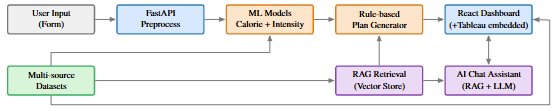
\includegraphics[width=\textwidth]{figures/system_architecture.png}
    \caption{Smart Workout system architecture.}
    \label{fig:system_architecture}
\end{figure}

The Smart Workout system is designed around a three-layer Business Intelligence (BI) framework consisting of descriptive, predictive, and prescriptive analytics. As shown in Figure~\ref{fig:system_architecture}, the process begins with a user input form which is processed via a FastAPI backend. The architecture integrates five public data sources represented as eight analytical tables or files to support these layers, helping the system move beyond mere data visualization to actionable guidance. This modular design allows for the independent validation of each stage, from initial data preprocessing to final plan generation and RAG-grounded explanations.

\subsection{Description of the Proposed DSS/BIS}

The proposed DSS/BIS is a web-based Smart Workout decision-support system that connects gym-operation analytics with personalized training guidance. At the business level, the system helps managers review branch utilization, estimated revenue contribution, subscription cohorts, lifestyle segments, and demand timing. At the individual level, the system helps gym members understand their readiness condition, predicted workout intensity, estimated calorie target, recommended weekly plan, and plan rationale. The DSS component is responsible for converting model and rule outputs into action recommendations, while the BIS component organizes operational, lifestyle, and training data into dashboard views that support monitoring and comparison. Therefore, the proposed system is not only a reporting dashboard; it is an integrated data-to-decision workflow that moves from raw data, to engineered features, to prediction, to prescriptive recommendation, and finally to dashboard-based action.


\section{Data Sources and Preprocessing}
\label{sec:data_sources}

The research utilizes five real-world public data sources, represented as eight tables or files, to ground the system in diverse fitness and lifestyle contexts, as summarized in Table~\ref{tab:datasets}. These include the Gym Database Management System for membership analytics (305,013 records), ExerciseDB for cataloging 1,500 exercises, and the Gym Members Exercise Tracking dataset (973 records) for training predictive models. Additionally, the Sleep Health \& Lifestyle and Daily Food Nutrition datasets provide the necessary context for user profiling and nutrition-aware guidance. All raw data underwent rigorous inspection, cleaning, and standardization to ensure consistency across the relational star schema and the vector store used for retrieval.

\begin{table}[htbp]
\centering
\small
\renewcommand{\arraystretch}{1.1}
\caption{Data sources used in the Smart Workout system.}
\label{tab:datasets}
\begin{tabularx}{\linewidth}{p{4.8cm}p{1.3cm}X}
\toprule
\textbf{Source table/file} & \textbf{Records} & \textbf{Role in the system} \\
\midrule
\href{https://www.kaggle.com/datasets/amoghabhinavms/gym-database-management-system}{Gym DB -- Users} (Amoghabhinavms, n.d.) & 5{,}000 & Member dimension table containing demographics, signup dates, locations, and subscription-plan keys. Supports dashboard filters and member segmentation. \\
\href{https://www.kaggle.com/datasets/amoghabhinavms/gym-database-management-system}{Gym DB -- Check-in/check-out history} (Amoghabhinavms, n.d.) & 300{,}000 & Central session fact table containing gym visits, workout type, timestamps, duration-derived features, and calories burned. Primary descriptive and warehouse source. \\
\href{https://www.kaggle.com/datasets/amoghabhinavms/gym-database-management-system}{Gym DB -- Subscription plans} (Amoghabhinavms, n.d.) & 3 & Plan dimension table containing monthly price and feature descriptions. Supports subscription mix and estimated recurring-revenue summaries. \\
\href{https://www.kaggle.com/datasets/amoghabhinavms/gym-database-management-system}{Gym DB -- Gym locations} (Amoghabhinavms, n.d.) & 10 & Location dimension table containing branch city, gym type, and facilities. Supports utilization analysis and location-level plan constraints. \\
\href{https://exercisedb.dev/}{ExerciseDB (raw flat)} (ExerciseDB, n.d.) & 1{,}500 & Exercise catalogue (body parts, equipment, target muscles, instructions). Supports the exercise recommender and RAG pipeline. \\
\href{https://www.kaggle.com/datasets/valakhorasani/gym-members-exercise-dataset}{Gym Members Exercise Tracking} (Khorasani, 2024) & 973 & Workout sessions with calories, BPM, duration, workout type, BMI, experience. Primary ML training data. \\
\href{https://www.kaggle.com/datasets/uom190346a/sleep-health-and-lifestyle-dataset}{Sleep Health \& Lifestyle} (Tharmalingam, 2023) & 374 & Informs lifestyle clustering and \emph{Training Readiness} rules derived from user input. \\
\href{https://www.kaggle.com/datasets/adilshamim8/daily-food-and-nutrition-dataset}{Daily Food Nutrition} (Shamim, 2025) & 651 & Macro/calorie context on the dashboard; nutrition-aware snippets embedded in RAG. \\
\bottomrule
\end{tabularx}

\end{table}

\section{Data Architecture and Schema Design}

\begin{figure}[H]
    \centering
    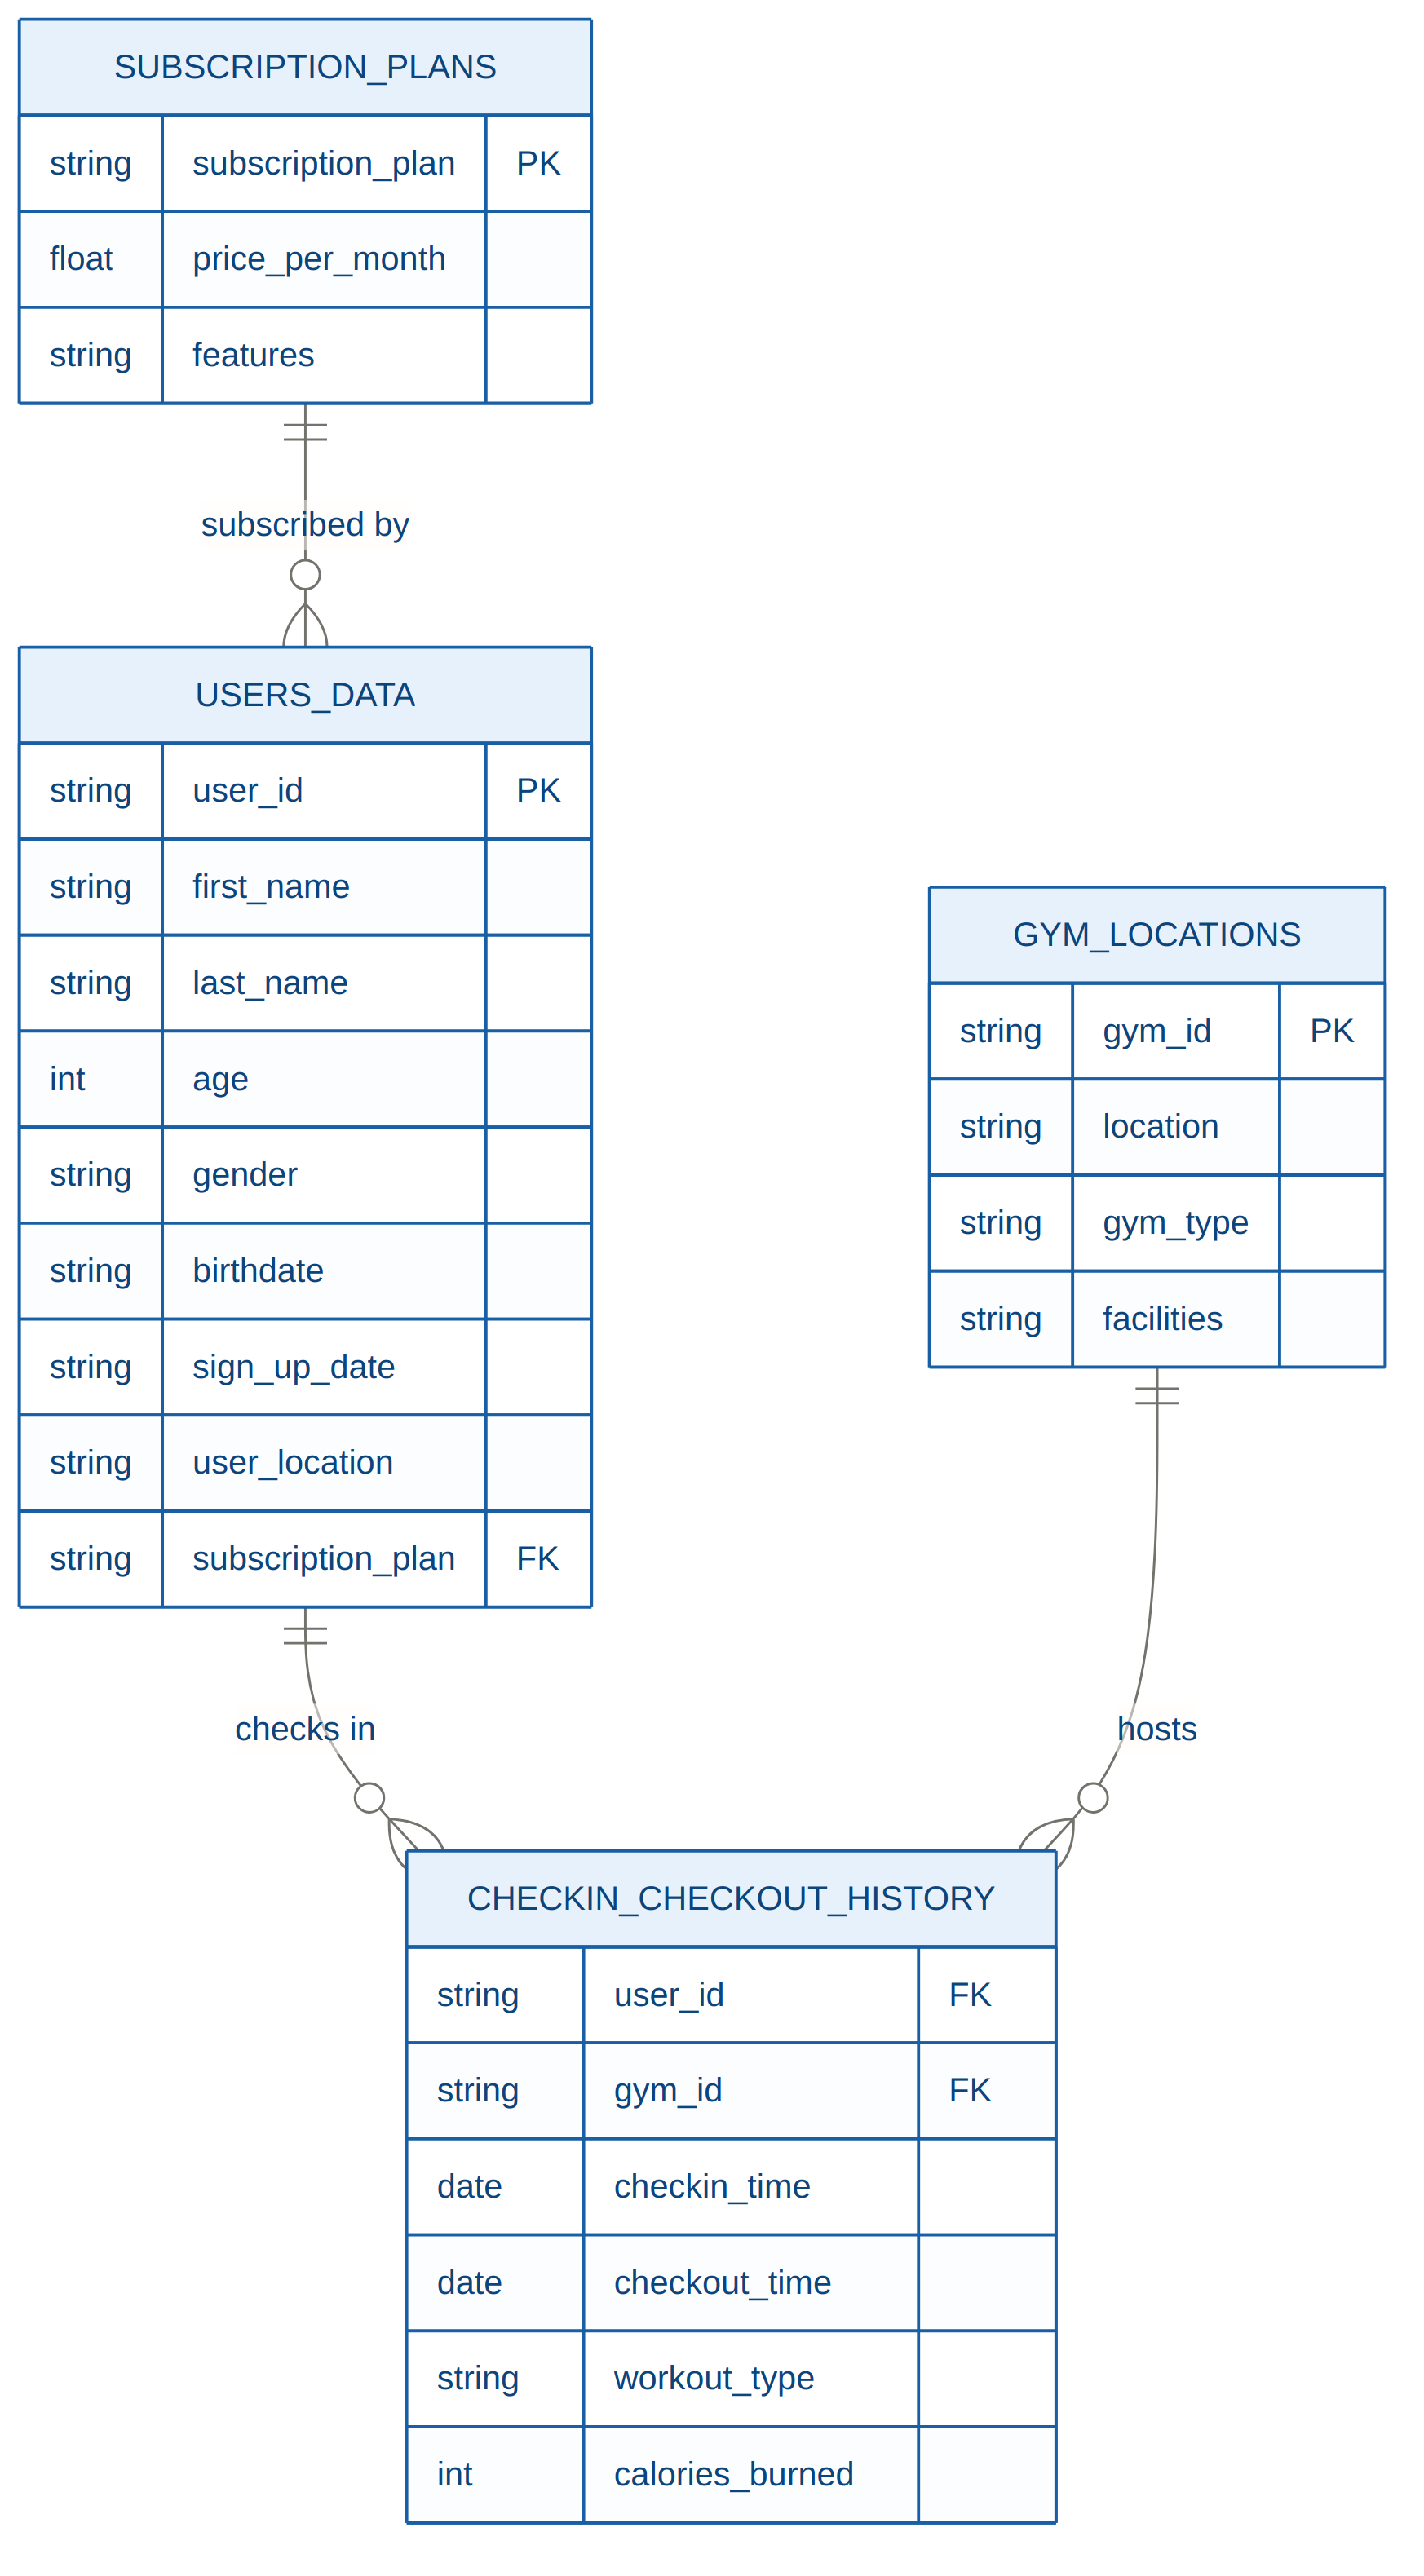
\includegraphics[width=0.7\linewidth]{figures/dataset_schema.png}
    \caption{Data architecture: connected and isolated datasets.}
    \label{fig:dataset_schema}
\end{figure}

\begin{figure}[H]
    \centering
    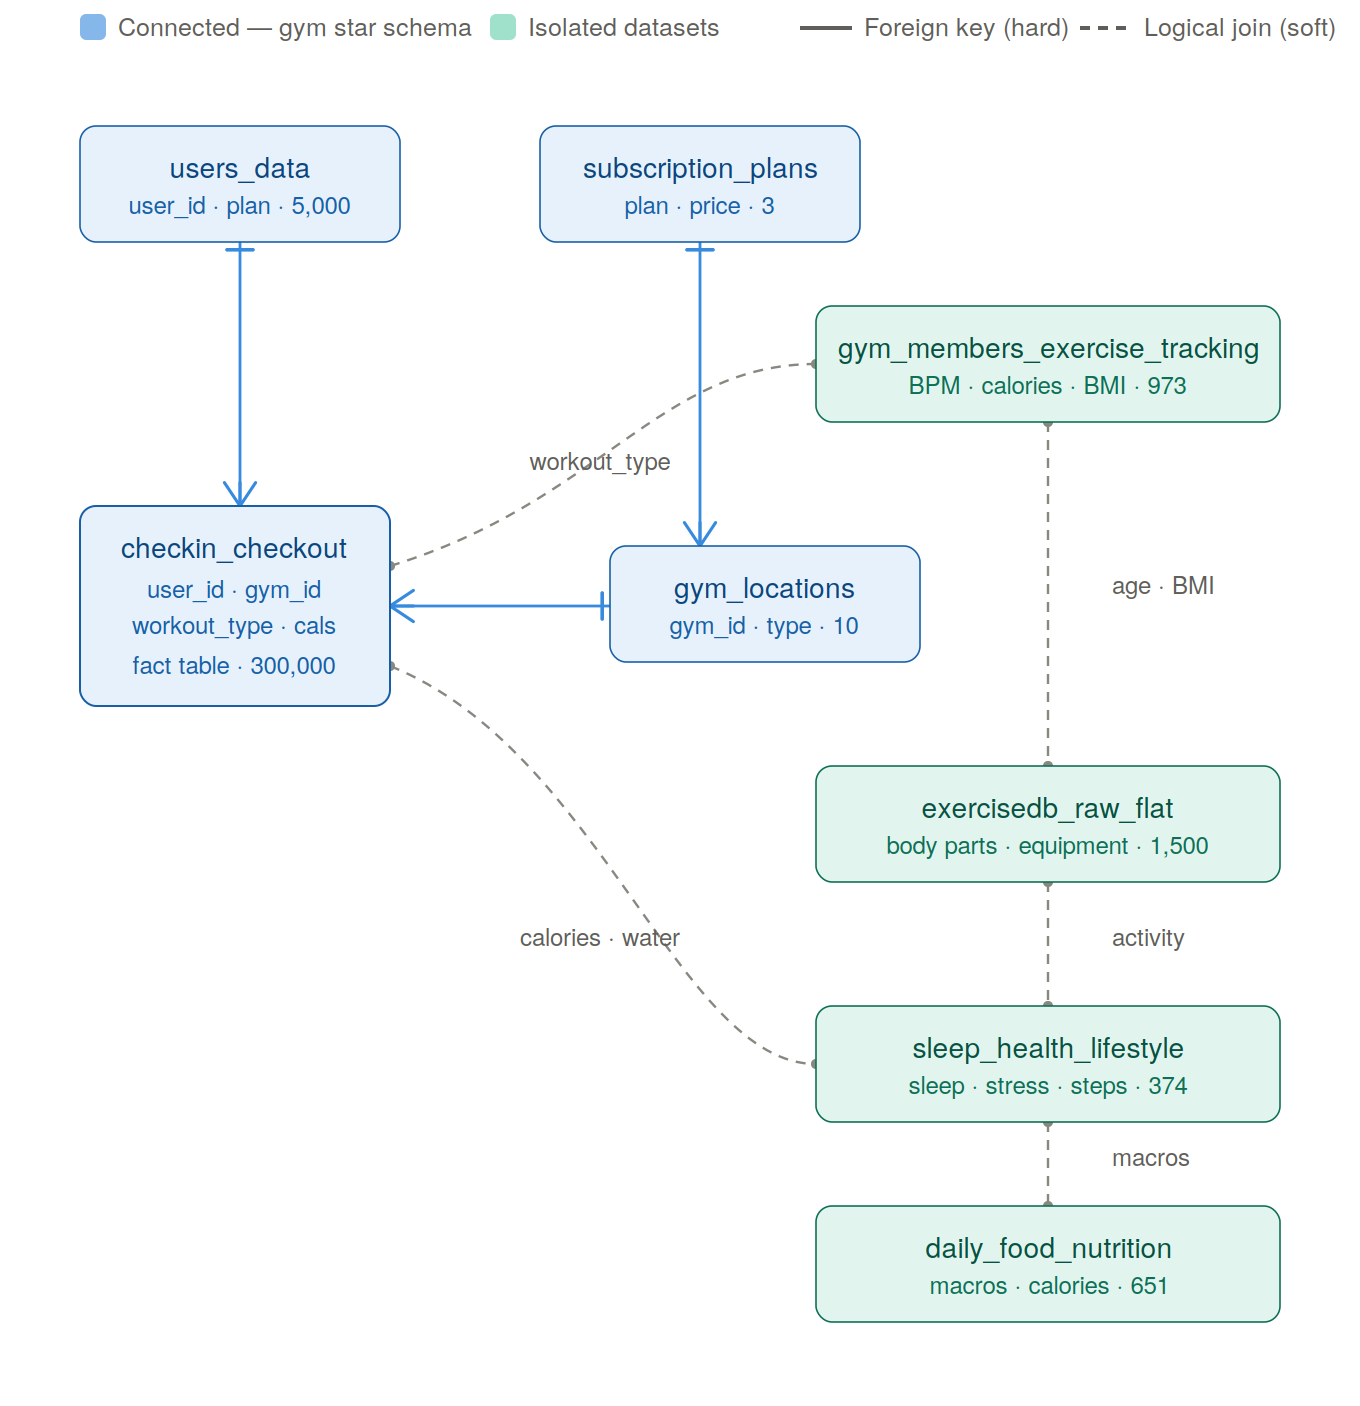
\includegraphics[width=\linewidth]{figures/gym_star_schema.png}
    \caption{Gym Database Management System star schema.}
    \label{fig:gym_star_schema}
\end{figure}

The integration of multi-source datasets within the Smart Workout system requires a structured architectural design to ensure data consistency across the descriptive, predictive, and prescriptive layers. This section details the logical and physical relationships between the various data components, ranging from the core relational gym database to the isolated datasets used for lifestyle clustering and RAG retrieval. The following diagrams illustrate the complexity of the data ecosystem and how independent sources are unified through either hard foreign keys or logical enrichment. These isolated sources provide population-level context rather than verified same-person joins. As shown in Figure~\ref{fig:dataset_schema}, the system utilizes an eight-table/file analytical schema that categorizes information into connected and isolated groups. The connected group forms the primary gym star schema, which tracks user demographics, subscription plans, and check-in history to support membership analytics. Conversely, isolated datasets such as ExerciseDB, Sleep Health \& Lifestyle, and Daily Food Nutrition are integrated via logical joins based on attributes such as workout type, age, and BMI. This design allows the system to combine macro-level lifestyle insights with micro-level exercise instructions to support evidence-based training plan generation.

The core of the descriptive analytics layer is supported by a relational star schema specifically designed for the Gym Database Management System, as illustrated in Figure~\ref{fig:gym_star_schema}. This schema centers on the \texttt{CHECKIN\_CHECKOUT\_HISTORY} fact table, which links to three primary dimension tables: \texttt{USERS\_DATA}, \texttt{SUBSCRIPTION\_PLANS}, and \texttt{GYM\_LOCATIONS}. By utilizing primary and foreign key relationships (e.g., \texttt{user\_id}, \texttt{gym\_id}, and \texttt{subscription\_plan}), the system can efficiently query more than 300,000 session records to identify utilization trends and subscription mix patterns. This relational foundation ensures that the BI dashboard provides a high-fidelity view of gym operations and member behavior.

\subsection{Lifestyle Archetype Clustering}

The lifestyle segments shown on the executive dashboard (\S\ref{sec:lifestyle_segment_result}) are produced by K-Means clustering on the Sleep Health \& Lifestyle dataset (374 records), using sleep duration, sleep quality, physical activity level, stress level, heart rate, and daily steps as clustering features. Candidate values of $k$ were compared by silhouette score, and $k=4$ was selected with a silhouette score of 0.464, against 0.393 for $k=3$. The dashboard displays each cluster with two labels layered together (Table~\ref{tab:cluster_profiles}): a statistical archetype label carried through from the clustering step, and a dashboard headline label computed independently by a small frontend threshold rule applied to each cluster's aggregate readiness score, stress level, and sleep duration (readiness $\geq 80$ and stress $\leq 4$: \emph{Performance-ready users}; readiness $\geq 65$: \emph{Stable habit users}; sleep $<6.5$h or stress $\geq 7$: \emph{Recovery-risk users}; otherwise: \emph{Habit-building users}).

\begin{table}[H]
\centering
\small
\caption{Lifestyle archetype clusters from K-Means ($k=4$) and their dashboard labels.}
\label{tab:cluster_profiles}
\begin{tabularx}{\linewidth}{cXXcc}
\toprule
\textbf{Cluster} & \textbf{Archetype label (clustering)} & \textbf{Dashboard headline label (frontend rule)} & \textbf{Records} & \textbf{Mean readiness score} \\
\midrule
0 & Moderate / Mixed Readiness & Habit-building users & 179 & 7.25 \\
1 & Strained / Low Recovery & Recovery-risk users & 32 & 2.97 \\
2 & Strained / Low Recovery & Recovery-risk users & 101 & 3.33 \\
3 & Moderate / Mixed Readiness & Habit-building users & 62 & 6.06 \\
\bottomrule
\end{tabularx}
\end{table}

The two ``Strained / Low Recovery'' clusters together account for 133 of 374 records (36\%) and combine short or irregular sleep with elevated stress and blood pressure, while the two ``Moderate / Mixed Readiness'' clusters show longer sleep duration and lower stress. This clustering result is what the readiness-band logic in \S\ref{sec:readiness_scoring} draws on conceptually: the same recovery signals (sleep, stress, blood pressure, resting heart rate) that separate these archetypes at the population level are the inputs to the per-user readiness score at inference time. One consequence of the readiness scale used at the clustering stage is that no cluster reaches the frontend rule's top two thresholds (readiness $\geq 65$ or $\geq 80$), so only the \emph{Recovery-risk} and \emph{Habit-building} headline labels are actually reachable for the current four clusters; \emph{Performance-ready} and \emph{Stable habit} remain defined in the rule but unused at this cluster resolution.

\section{Predictive Modeling Pipeline}
\label{sec:predictive_pipeline}

The predictive layer employs a best-of-three model selection strategy for two primary tasks: calorie-burn-rate regression and workout-intensity classification. For the regression task, candidates include Ridge Regression, Random Forest Regressor, and XGBoost Regressor, with selection based on minimizing Root Mean Square Error (RMSE). The classification task evaluates Multinomial Logistic Regression, Random Forest, and XGBoost to categorize intensity into three levels (Low, Mid, High). Models are evaluated using 5-fold cross-validation to ensure generalizability, and SHAP (SHapley Additive exPlanations) is applied to the selected models to provide transparency regarding which physiological features most heavily influence the predictions.

Both supervised targets are themselves derived fields rather than raw columns in the Gym Members Exercise Tracking dataset. The regression target is calories burned normalized by session length:
\begin{equation}
r_{kcal/hr}=\frac{\text{calories\_burned}}{\text{session\_duration\_hours}}
\end{equation}
and the classification target is a three-way binning of the ratio between average and maximum heart rate observed during the session:
\begin{equation}
\text{intensity\_band}=
\begin{cases}
\text{Low} & \text{avg\_bpm}/\text{max\_bpm}\leq0.70\\
\text{Mid} & 0.70<\text{avg\_bpm}/\text{max\_bpm}\leq0.85\\
\text{High} & \text{avg\_bpm}/\text{max\_bpm}>0.85
\end{cases}
\end{equation}
This is the same \texttt{bpm\_response\_ratio} quantity listed as a regression feature in Table~\ref{tab:feature_provenance}; here it defines the classification label itself rather than an input feature. The selected calorie estimation model is trained to estimate calorie-burn rate, not total session calories. The system then converts the estimated hourly rate into a practical session target using the planned workout duration:
\begin{equation}
\widehat{C}_{session}=\widehat{r}_{kcal/hr}\times d_{hours}
\end{equation}
where $\widehat{r}_{kcal/hr}$ is the predicted calorie-burn rate and $d_{hours}$ is the prescribed session duration. Training readiness is computed as a rule-derived score from recovery and lifestyle inputs, then combined with predicted intensity to determine the final plan level:
\begin{equation}
S_{plan}=0.60S_{readiness}+0.40S_{intensity}
\end{equation}
The 0.60/0.40 weighting is a design heuristic that prioritizes recovery readiness over predicted intensity; it should be recalibrated with real adherence and outcome data in future work. A readiness cap is applied whenever recovery is not fully High (i.e. for the Low and Medium readiness bands, detailed in \S\ref{sec:readiness_scoring}) so that the prescribed volume cannot exceed the user's current recovery condition, even if the predicted intensity class is high.

XGBoost is used because boosted decision trees can model non-linear interactions among body composition, workout type, and heart-rate features. Its simplified objective can be written as:
\begin{equation}
\mathcal{L}^{(t)}=\sum_{i=1}^{n}l\left(y_i,\hat{y}_i^{(t-1)}+f_t(x_i)\right)+\Omega(f_t), \quad
\Omega(f)=\gamma T+\frac{1}{2}\lambda\sum_{j=1}^{T}w_j^2
\end{equation}
where $f_t$ is the tree added at iteration $t$, $T$ is the number of leaves, and $w_j$ is a leaf weight. Random Forest is retained as a benchmark because it averages many decorrelated trees:
\begin{equation}
\hat{y}_{RF}=\frac{1}{B}\sum_{b=1}^{B}T_b(x)
\end{equation}
for regression, while classification uses the majority vote across trees. These equations support the model comparison rather than implying that every candidate is used at inference time.

\begin{table}[htbp]
\centering
\small
\caption{Predictive layer input, output, and result mapping.}
\label{tab:ml_input_output}
\begin{tabularx}{\linewidth}{p{3.2cm}p{4.4cm}p{3.2cm}X}
\toprule
\textbf{Task} & \textbf{Input variables} & \textbf{Output} & \textbf{Selected result} \\
\midrule
Calorie-burn-rate regression & Numerical: age, weight, height, max BPM, average BPM, resting BPM, fat percentage, water intake, workout frequency, experience level, BMI, BPM response ratio. Categorical: workout type, intensity band. & kcal/hr estimate and session calorie target & XGBoost Regressor, RMSE 15.021 kcal/hr, MAE 10.424 kcal/hr, $R^2=0.970$. \\[10pt]
Workout-intensity classification & Numerical: age, weight, height, resting BPM, fat percentage, water intake, workout frequency, experience level, BMI. Categorical: workout type. & Low, Mid, or High intensity class & XGBoost Classifier, accuracy 0.399 and macro-F1 0.342 after class-balancing. \\[10pt]
Prescriptive plan mapping & Predicted intensity, readiness score, readiness band, goal, equipment, target body part, constraints, and available schedule. & Sets, reps, rest seconds, weekly schedule, safety notes, and primary action & Rule-based plan output capped by readiness and grounded by RAG-retrieved exercise evidence. \\
\bottomrule
\end{tabularx}
\end{table}

\begin{table}[htbp]
\centering
\small
\caption{Feature handling in the predictive layer.}
\label{tab:feature_types}
\begin{tabularx}{\linewidth}{p{3cm}p{4.4cm}X}
\toprule
\textbf{Feature type} & \textbf{Examples} & \textbf{Processing and reporting role} \\
\midrule
Numerical inputs & \texttt{age}, \texttt{weight\_kg}, \texttt{height\_m}, \texttt{resting\_bpm}, \texttt{fat\_percentage}, \texttt{water\_intake\_liters}, \texttt{bmi} & Passed through model preprocessing and used in SHAP explanation charts so users can see which body-composition or recovery factors influence the prediction. \\[10pt]
Categorical inputs & \texttt{workout\_type}, \texttt{intensity\_band} for regression only & One-hot encoded before model training. Gender is excluded because the deployed form does not collect gender, preventing train/inference mismatch. \\[10pt]
Numerical outputs & Calorie-burn-rate estimate, session calorie target, readiness score, final training score, sets, reps, rest seconds, exercise count & Reported as measurable plan and dashboard values that support calorie targeting, workload control, and weekly progress monitoring. \\[10pt]
Categorical outputs & Predicted Low/Mid/High intensity class, readiness band, priority action, target body-part focus, equipment fit, plan rationale category & Reported as interpretable labels that guide user-facing recommendations and executive decision signals. \\
\bottomrule
\end{tabularx}
\end{table}

\begin{table}[H]
\centering
\small
\caption{Deployment-time provenance of predictive-layer features.}
\label{tab:feature_provenance}
\begin{tabularx}{\linewidth}{p{2.8cm}p{5.2cm}X}
\toprule
\textbf{Provenance} & \textbf{Features} & \textbf{Note} \\
\midrule
Directly collected on the form & \texttt{age}, \texttt{weight\_kg}, \texttt{height\_m}, \texttt{resting\_bpm}, \texttt{workout\_frequency\_} \texttt{days\_week} & Used as reported, with no estimation step. \\[10pt]
Exact derivation from collected values & \texttt{bmi} & Computed with the standard formula; not a heuristic guess. \\[10pt]
Rule-based estimate at inference & \texttt{max\_bpm}, \texttt{avg\_bpm}, \texttt{fat\_percentage}, \texttt{water\_intake\_liters}, \texttt{workout\_type}, \texttt{experience\_level}, \texttt{bpm\_response\_ratio}, \texttt{intensity\_band} (regression only) & Not collected by the deployment form; each is approximated with a simple rule (age/stress for max BPM, a heart-rate-reserve ratio keyed to intensity for average BPM, a BMI/age/goal bucket for fat percentage, a weight-based formula for water intake, a goal/body-part lookup for workout type, session-count buckets for experience level). \\
\bottomrule
\end{tabularx}
\end{table}

Table~\ref{tab:feature_provenance} extends the average-BPM caveat discussed in \S\ref{sec:model_selection}: it is not an isolated exception but the most consequential instance of a broader pattern, since average BPM is also the regressor's top SHAP feature. Roughly half of the regression feature set is rule-estimated rather than measured at inference, and this provenance gap is disclosed here so that Chapter 4's model-selection results can be read against what is actually observed in deployment versus what is approximated.

\section{RAG and Prescriptive Plan Generation}

The prescriptive layer combines a rule-based engine with a Retrieval-Augmented Generation (RAG) knowledge layer to generate personalized training plans. The RAG system utilizes ChromaDB and sentence embeddings (all-MiniLM-L6-v2) to index exercise instructions and equipment substitution rules. When a user submits their profile, the rule-based generator integrates the predicted intensity, the calculated training readiness band, and target body parts to filter the ExerciseDB pool. This helps make the resulting daily or weekly plans specific to the user's goals while keeping the rationale grounded in evidence retrieved from the knowledge base.

\subsection{Readiness Scoring, Volume Capping, and Exercise-Match Rules}
\label{sec:readiness_scoring}

The readiness score itself is produced by an additive, rule-based deduction model rather than a learned model, so its logic is fully transparent and auditable. Starting from a baseline of 100, the score is reduced by a fixed penalty whenever a recovery or safety signal falls outside its healthy range:
\begin{equation}
S_{readiness}=\max\Big(0,\ 100-\sum_{k}p_k\cdot\mathbf{1}[\text{signal}_k\text{ out of range}]\Big)
\end{equation}
where $p_k$ is the penalty weight for signal $k$: sleep duration below 6 hours ($p=25$), stress level of 8 or above ($p=15$; a moderate stress level of 5--7 uses $p=8$), elevated blood pressure at or above 140/90 mmHg ($p=20$), resting heart rate above 90 bpm ($p=15$), and BMI at or above 30 ($p=10$). The resulting score is mapped to a readiness band: High ($S_{readiness}\geq80$), Medium ($55\leq S_{readiness}<80$), or Low ($S_{readiness}<55$).

To keep the 60/40 readiness-intensity blend from overriding a low readiness signal, a band-conditioned cap is applied after the blend is computed:
\begin{equation}
S_{plan}^{capped}=
\begin{cases}
\min(S_{plan},\,54) & \text{readiness band}=\text{Low} \\
\min(S_{plan},\,84) & \text{readiness band}=\text{Medium} \\
S_{plan} & \text{readiness band}=\text{High}
\end{cases}
\end{equation}
This prevents a high predicted-intensity class from pushing the recommendation into a higher training-volume tier than the user's current recovery condition supports.

Exercise candidates within the body-part- and equipment-filtered ExerciseDB pool are ranked with a lightweight match score, which the dashboard surfaces as a percentage next to each recommended exercise (Figure~\ref{fig:chapter4_exercise_plan}):
\begin{multline}
\text{match\_score}=\min\big(1.0,\ 0.70+0.20\cdot\mathbf{1}[\text{equipment exact match}] \\
{}+0.10\cdot\mathbf{1}[\text{body-part match}]\big)
\end{multline}
Every candidate already satisfies the target body-part filter, so the 0.70 base reflects that minimum body-part fit; the two bonus terms reward an exact equipment match and additional body-part specificity. For a specific target body part this gives a maximum displayed match of 100\%; for a ``full body'' target the body-part bonus does not apply (no single body part is being matched against), so the maximum displayed match is 90\% in that case. This is a rule-based coverage/fit heuristic, not a semantic similarity score from the RAG retriever, and should be read as ``how well this exercise fits the stated equipment and target area'' rather than as retrieval relevance.

The retrieval mechanism itself operates in one of two modes depending on deployment configuration. In vector mode, the user query is embedded with the same all-MiniLM-L6-v2 sentence-transformer used to build the index, and ChromaDB returns the nearest documents by embedding similarity. In keyword mode, retrieval instead uses a lexical overlap score, ranking curated rule snippets by the count of shared lowercase word-stems between the query and each snippet, without computing any embedding. Keyword mode is the default for the live deployment (\texttt{RAG\_MODE=keyword} in \texttt{render.yaml}) because it avoids loading the sentence-transformer model on the free-tier host, reducing first-request latency and memory pressure; vector mode remains available for local development and can be enabled where more memory headroom exists. In practice, this means the deployed system's retrieval is lexical rather than semantic by default, which is a scope detail worth stating explicitly rather than leaving implied by the architecture description alone.

\subsection{Plan Volume and Recommendation-Level Rules}

The base training prescription for each predicted intensity class is a fixed sets/reps/rest triple (Low: 2 sets, 10--12 reps, 75s rest; Medium: 3 sets, 8--12 reps, 90s rest; High: 4 sets, 6--10 reps, 120s rest). The generator then adjusts this triple by goal and readiness: rep ranges shift toward higher reps for fat loss and lower reps for strength; rest is extended for strength (+20s) and shortened for fat loss (--15s) and general fitness (--5s), with a further +15s whenever readiness is Low; and set count drops by one (minimum two) when readiness is Low and rises by one when readiness and predicted intensity are both High.

The capped plan score from \S\ref{sec:readiness_scoring} is separately mapped to a recommendation-level label (Table~\ref{tab:recommendation_levels}), while the volume multiplier and primary action shown on the dashboard are set directly from readiness band and predicted intensity, evaluated in the order listed in Table~\ref{tab:volume_multiplier} (first match applies).

\begin{table}[H]
\centering
\small
\caption{Recommendation-level bands from the capped plan score.}
\label{tab:recommendation_levels}
\begin{tabularx}{\linewidth}{Xl}
\toprule
\textbf{Condition (evaluated top to bottom)} & \textbf{Recommendation level} \\
\midrule
Readiness High, predicted intensity High, and capped score $\geq 85$ & Performance / Advanced \\
Capped score $<55$ & Recovery / Light \\
$55 \leq$ capped score $<70$ & Foundation / Controlled \\
Capped score $\geq 70$ (otherwise) & Progressive / Standard \\
\bottomrule
\end{tabularx}
\end{table}

\begin{table}[H]
\centering
\small
\caption{Volume multiplier and primary action from readiness band and predicted intensity.}
\label{tab:volume_multiplier}
\begin{tabularx}{\linewidth}{p{4.4cm}lX}
\toprule
\textbf{Condition (evaluated top to bottom)} & \textbf{Multiplier} & \textbf{Primary action} \\
\midrule
Readiness Low & 0.75$\times$ & Reduce sets or exercise count, keep movement controlled, extend rest. \\
Readiness High and predicted High & 1.15$\times$ & Allow the full high-intensity plan at the highest safe volume. \\
Predicted High (readiness not Low or High-High) & 1.05$\times$ & Use higher workload, but keep readiness checks active before adding volume. \\
Predicted Low (readiness not Low) & 0.90$\times$ & Prioritize technique, lower-impact choices, and gradual progression. \\
Otherwise (predicted Medium) & 1.00$\times$ & Use the standard progression for the selected goal and focus area. \\
\bottomrule
\end{tabularx}
\end{table}

\section{System Implementation and Deliverables}

The final implementation is delivered as a full-stack web application utilizing React for the frontend and FastAPI for the backend orchestration. The dashboard features embedded Tableau views for relational membership analytics and lifestyle profiling, alongside custom React components for displaying prediction results and the generated workout plan. Key deliverables of this methodology include the working prototype, the validated machine learning endpoints, and the RAG-assisted chat interface. This integrated technology stack enables the system to provide a seamless transition from descriptive insight to predictive estimation and, ultimately, prescriptive action.

\subsection{Backend Implementation}

\begin{figure}[H]
    \centering
    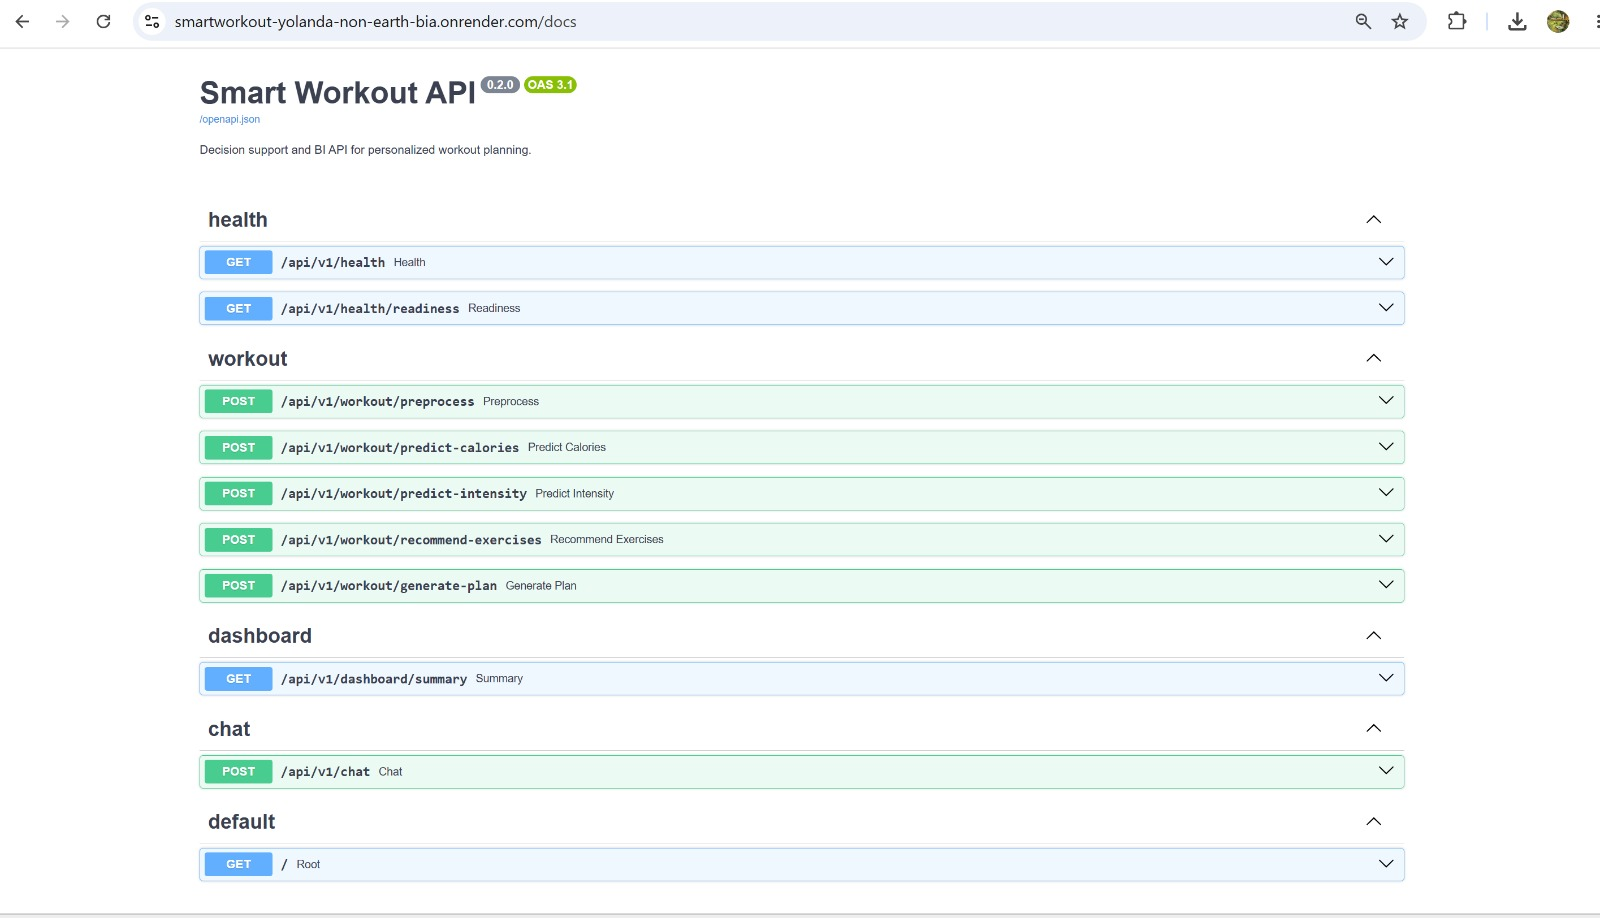
\includegraphics[width=0.92\linewidth]{figures/Backend.jpeg}
    \caption{Backend implementation.}
    \label{fig:backend_implementation}
\end{figure}

The backend was implemented with FastAPI as the orchestration layer for the Smart Workout system. It receives profile and dashboard requests from the React frontend, prepares the required inputs, calls the machine-learning and RAG components, and returns structured outputs for the dashboard, plan generator, and assistant interface. Figure~\ref{fig:backend_implementation} summarizes the backend implementation used in the prototype.

\subsection{Tableau Map Integration}

The Tableau integration was completed in the React dashboard as an embedded map panel. The implementation uses an iframe to load the Tableau Public gym-location view and places it beside location-level utilization summaries. Bubble size represents session volume, colour represents gym type, and the surrounding React dashboard provides filters and KPI context. Tableau supplies the interactive geospatial visual, while React and FastAPI supply the broader decision-support workspace; the map itself and its geographic findings are presented as a results artifact in \S\ref{sec:dashboard_results}, alongside the executive summary it is designed to complement.

This chapter has presented the comprehensive methodology for constructing a data-driven decision support tool for weight training. The methods described, ranging from multi-source data cleaning to the deployment of boosted-tree models and vector databases, address the limitations of generic, non-adaptive training plans identified in earlier chapters. Among these methods, the integration of RAG-grounded AI provides the distinct advantage of delivering evidence-based explanations alongside prescriptive plans. These methodological steps ensure that the results and discussions presented in Chapter 4 are based on a robust, validated, and transparent system architecture.

% ==================== CHAPTER 4 ====================
\chapter{RESULTS AND DISCUSSION}

This chapter presents the implemented results of Smart Workout, following the same descriptive-predictive-prescriptive progression introduced in Chapters 1 and 2. \S4.1 reports the \emph{descriptive} dataset and feature-engineering evidence; \S4.2 reports the \emph{predictive} model-selection results; \S4.3 shows the dashboard where all three layers are integrated and evaluated in business and user context, including the \emph{prescriptive} plan-generation output; and \S4.4 closes the chapter with the RAG-grounded explanation layer that grounds those prescriptive plans in retrieved evidence. To avoid repeating appendix material, detailed EDA plots are placed in Appendix B, while this chapter focuses on the meaning of the results and how they support business and user decisions.

\section{Dataset and Feature Engineering Results}

The dataset preparation stage produced several feature-engineering results that became the input to the dashboard, predictive models, and plan-generation workflow. Instead of using the raw datasets directly, the system transformed visit records, membership records, exercise-tracking records, lifestyle records, and user-profile inputs into decision-ready variables. These engineered results are important because they connect the raw data sources to the actual business and user questions addressed in the dashboard.

\begin{table}[htbp]
\centering
\small
\caption{Feature-engineering results in the final system.}
\label{tab:feature_engineering_results}
\begin{tabularx}{\linewidth}{p{3.5cm}p{4.1cm}X}
\toprule
\textbf{Engineered result} & \textbf{Main derived fields} & \textbf{Dashboard or model usage} \\
\midrule
Utilization and time features & Session month, check-in hour, weekday/weekend pattern, branch session count & Used to compare demand by location and time period, detect overloaded or underused capacity, and support staffing or campaign decisions. \\
Membership and revenue signals & Subscription tier, plan mix, estimated monthly recurring revenue, cohort-level activity & Used to compare utilization with estimated revenue share and identify retention or upsell opportunities by cohort. \\
Lifestyle readiness features & Readiness score, readiness band, sleep/stress/activity indicators, lifestyle segment & Used to explain wellness risk, prioritize recovery interventions, and personalize plan intensity. \\
Workout-intensity features & Workout type, avg BPM proxy, resting BPM, body-composition features, intensity band & Used by the classifier to predict Low, Mid, or High intensity and by the dashboard to explain which user inputs influence the plan. \\
Calorie-burn-rate target & Calories normalized as kcal/hr, with session duration excluded from regression features & Used by the regressor to estimate calorie-burn rate without directly learning from session length. \\
Plan decision features & Predicted intensity, readiness cap, final training score, primary action & Used to convert prediction results into sets, reps, rest periods, exercise count, and weekly adjustment guidance. \\
RAG retrieval features & Goal, target body part, equipment, readiness band, predicted intensity & Used to retrieve relevant exercises and explanation snippets for personalized plan rationale and chat responses. \\
\bottomrule
\end{tabularx}
\end{table}

The feature-engineering result shows that Smart Workout is not only a visualization of raw records. It converts operational data into utilization and revenue signals, converts lifestyle and profile data into readiness signals, and converts model outputs into plan-decision variables. This allows the executive dashboard to answer where action is needed, while the user dashboard explains why a specific plan, intensity level, and weekly adjustment were recommended.

The EDA findings are summarized briefly here because the detailed EDA figures are placed in Appendix B. Overall, the EDA showed uneven utilization across gym locations, clear time-of-day demand patterns, visible subscription and workout-type differences, and imbalanced intensity classes. These patterns justify the dashboard filters, the branch-level decision panels, the readiness segmentation, and the decision to evaluate the classifier with macro-F1 rather than accuracy alone.
\section{Model Selection}
\label{sec:model_selection}

The predictive layer contains two machine learning tasks. The first task estimates calorie-burn rate in kcal/hr, and the second task predicts workout intensity as a three-class label: Low, Mid, or High. Model selection used 5-fold cross-validation and compared a linear baseline, Random Forest, and XGBoost for each task. The regressor is selected on lowest RMSE, while the classifier is selected on highest macro-F1 rather than accuracy because the intensity classes are imbalanced and accuracy would reward a model that simply predicts the majority Mid class.

\begin{table}[htbp]
\centering
\small
\caption{Regression model comparison for calorie-burn-rate estimation.}
\label{tab:chapter4_regression_results}
\begin{tabular}{lrrrl}
\toprule
\textbf{Model} & \textbf{RMSE} & \textbf{MAE} & \textbf{$R^2$} & \textbf{Selected} \\
\midrule
Ridge Regression & 28.095 & 22.524 & 0.895 & No \\
Random Forest Regressor & 17.991 & 11.457 & 0.957 & No \\
XGBoost Regressor & 15.021 & 10.424 & 0.970 & Yes \\
\bottomrule
\end{tabular}
\end{table}

The XGBoost Regressor is selected because it produces the strongest calorie-burn-rate estimation result, with RMSE 15.021 kcal/hr and $R^2=0.970$ on cross-validated folds. This result is reported as a deployment-aware upper bound rather than a guaranteed operational score. Gender was removed to prevent a train/inference mismatch, and features that created misleading training-time advantage were corrected. One caveat remains: the highest-attribution feature in the SHAP analysis (Figure~\ref{fig:appendix_calorie_shap}) is average BPM, which is estimated from predicted intensity at deployment rather than measured directly. Therefore, a version of the model that excludes average BPM or substitutes the deployment-time estimate during training and evaluation is required before the $R^2=0.970$ figure can be treated as fully operational.

\begin{table}[htbp]
\centering
\small
\caption{Classifier comparison with trivial baselines; XGBoost is selected on macro-F1.}
\label{tab:chapter4_classifier_results}
\begin{tabular}{lrrl}
\toprule
\textbf{Model} & \textbf{Accuracy} & \textbf{Macro-F1} & \textbf{Selected} \\
\midrule
Majority-class baseline (always Mid) & 0.525 & 0.229 & -- \\
Stratified-random baseline & $\approx$0.400 & $\approx$0.333 & -- \\
Multinomial Logistic Regression & 0.323 & 0.298 & No \\
Random Forest Classifier & 0.407 & 0.337 & No \\
XGBoost Classifier & 0.399 & 0.342 & Yes \\
\bottomrule
\end{tabular}
\end{table}

The classifier result requires careful interpretation and is deliberately reported against baselines rather than in isolation. The selected XGBoost Classifier reaches accuracy 0.399 and macro-F1 0.342 on cross-validated out-of-fold predictions. A majority-class classifier that always predicts Mid reaches higher raw accuracy, approximately 0.525, but only 0.229 macro-F1 because it never recovers the Low or High classes. A stratified-random baseline reaches approximately 0.333 macro-F1. XGBoost therefore loses to the majority baseline on accuracy but beats both trivial baselines on macro-F1, which is why macro-F1 is the selection metric for this imbalanced three-class task.

Per-class recall for the selected model, computed from the cross-validated XGBoost confusion matrix in Figure~\ref{fig:confusematrix}, is Low 21.5\%, Mid 51.9\%, and High 29.3\%. Minority-class recovery remains the weakest point, especially for Low intensity. The margin between XGBoost macro-F1 0.342 and Random Forest macro-F1 0.337 is also small, so XGBoost is retained as the final model because it has the highest macro-F1 in the exported cross-validation result and fits the selected SHAP-based explanation pipeline, not because the difference is large.

\begin{table}[htbp]
\centering
\small
\caption{Predictive layer audit summary after model and inference fixes.}
\label{tab:chapter4_predictive_audit}
\begin{tabularx}{\linewidth}{p{3.3cm}p{4cm}X}
\toprule
\textbf{Audit item} & \textbf{Issue found} & \textbf{Result after correction} \\
\midrule
Gender feature mismatch & Training used Male/Female, while inference sent an unknown value because the form does not ask for gender. & Gender was removed from both training and inference feature sets, preventing train/inference distribution mismatch. \\[10pt]
Classifier imbalance & Mid class was the majority class, so the model under-predicted Low and High intensity. & Balanced class weighting improved macro-F1 from 0.316 to 0.342. The final model beats majority-class and stratified-random baselines on macro-F1 but remains below the majority baseline on accuracy; per-class recall is Low 21.5\%, Mid 51.9\%, and High 29.3\%. \\[10pt]
Joblib deserialization risk & A custom XGBoost wrapper defined inside the training script serialized with an unstable class path. & The wrapper was moved to \path{app.core.ml_wrappers.BalancedXGBClassifier}, making model loading stable in the backend. \\[10pt]
Inflated regression score & Some training features made the regression score appear too optimistic under deployment conditions. & The deployment-aware cross-validated result is $R^2=0.970$ and RMSE 15.021 kcal/hr, but this is treated as an upper bound because average BPM is estimated at inference rather than directly observed. \\
\bottomrule
\end{tabularx}
\end{table}

The key model-selection conclusion is that the final predictive layer prioritizes transparent reporting over inflated headline scores. The regression model can support calorie-target guidance, but its $R^2=0.970$ should be read as an upper bound until average BPM is handled under the same derivation protocol in training and deployment. The classifier is only partially successful: it improves macro-F1 over trivial baselines but remains below the majority baseline on raw accuracy and still under-recovers minority classes. This is reported directly because the system is intended for decision support, where understanding model limitations is more useful than hiding them.

\section{Dashboard}
\label{sec:dashboard_results}

The dashboard is the main delivery layer of the project. It connects descriptive analytics, predictive outputs, and prescriptive recommendations into one React and FastAPI workflow. The executive view focuses on branch, segment, month, utilization, and revenue-share decisions. The user view focuses on readiness, predicted intensity, calorie target, and personalized plan interpretation. The following dashboard figures are all new captures from the implemented dashboard and are used once in this chapter.

\begin{figure}[H]
    \centering
    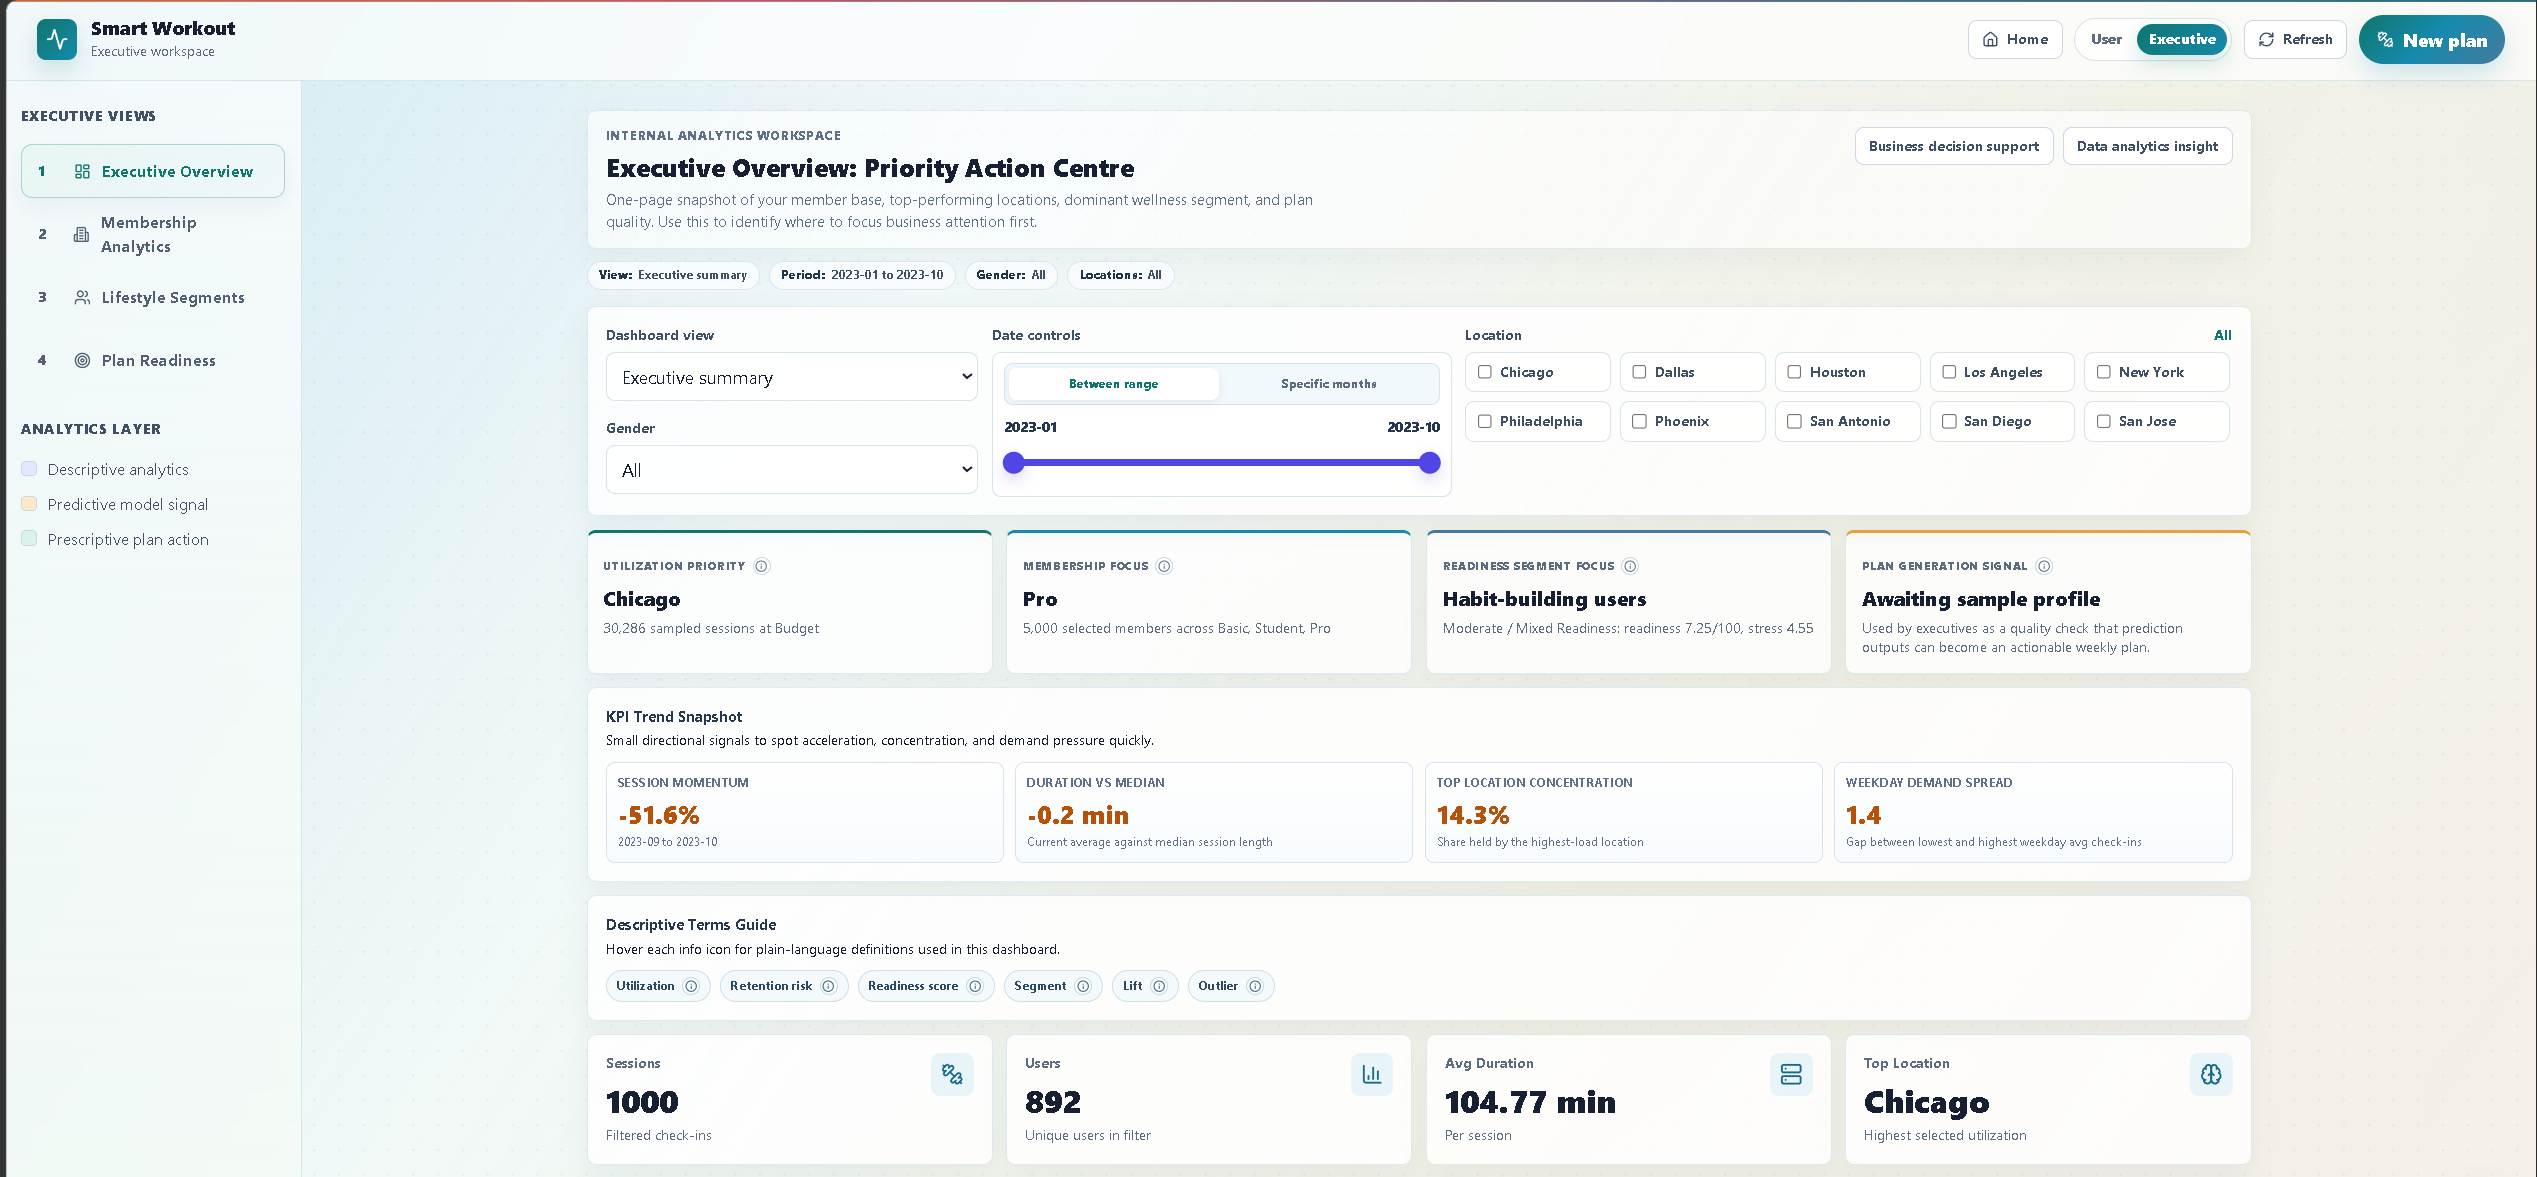
\includegraphics[width=0.95\linewidth]{figures/fig_dashboard_overview_controls.png}
    \caption{Dashboard navigation shell: view menu, analytics-layer legend, and workspace switch.}
    \label{fig:chapter4_dashboard_shell}
\end{figure}

Before reviewing individual views, Figure~\ref{fig:chapter4_dashboard_shell} orients the reader in the overall navigation structure. All dashboard content in this chapter is reached through this shell: the sidebar switches between the four executive views, the analytics-layer legend signals whether a panel is descriptive, predictive, or prescriptive, and the top-right toggle switches between the executive and individual-user workspaces without leaving the application.

\begin{table}[htbp]
\centering
\small
\caption{Business question, dashboard visual, and action decision mapping.}
\label{tab:chapter4_business_visual_action}
\begin{tabularx}{\linewidth}{p{4.2cm}p{3.6cm}X}
\toprule
\textbf{Business question} & \textbf{Dashboard visual} & \textbf{Action decision} \\
\midrule
Which locations, segments, and months contribute the highest utilization and estimated revenue share? & Executive summary, Tableau map, and membership revenue signals & Prioritize branch-level staffing, retention, or campaign review for high-impact locations and cohorts. \\[18pt]
\hline\\[-8pt]
Where do demand patterns indicate overload or underused capacity? & Executive utilization and time-pattern views & Adjust staffing schedules, class slots, or branch-level promotions. \\[18pt]
\hline\\[-8pt]
Which lifestyle segments have the largest member share and lowest readiness? & Member lifestyle segment dashboard & Prioritize recovery, low-intensity, or habit-building interventions. \\[18pt]
\hline\\[-8pt]
How different are weekday and weekend check-in patterns? & Date controls, utilization views, and Appendix B EDA & Shift campaigns, class times, or operational staffing by day type. \\[18pt]
\hline\\[-8pt]
Which subscription cohorts have retention risk or upsell potential? & Membership utilisation and revenue signals & Target low-engagement cohorts for retention and high-engagement cohorts for upgrade offers. \\[18pt]
\hline\\[-8pt]
Are prediction-to-plan outputs consistent with observed descriptive behavior? & Client inputs, exercise plan analytics, and member profile outputs & Audit whether model outputs align with branch, segment, and tier behavior before using recommendations operationally. \\
\bottomrule
\end{tabularx}
\end{table}

\subsection{Executive Dashboard Result}

The executive dashboard turns gym activity into business-level monitoring. It answers which branches, customer segments, months, and subscription cohorts should receive attention first. The before-state capture shows the base executive context, while the updated executive summary views show the final KPI and decision layout after the dashboard redesign.

\begin{figure}[H]
    \centering
    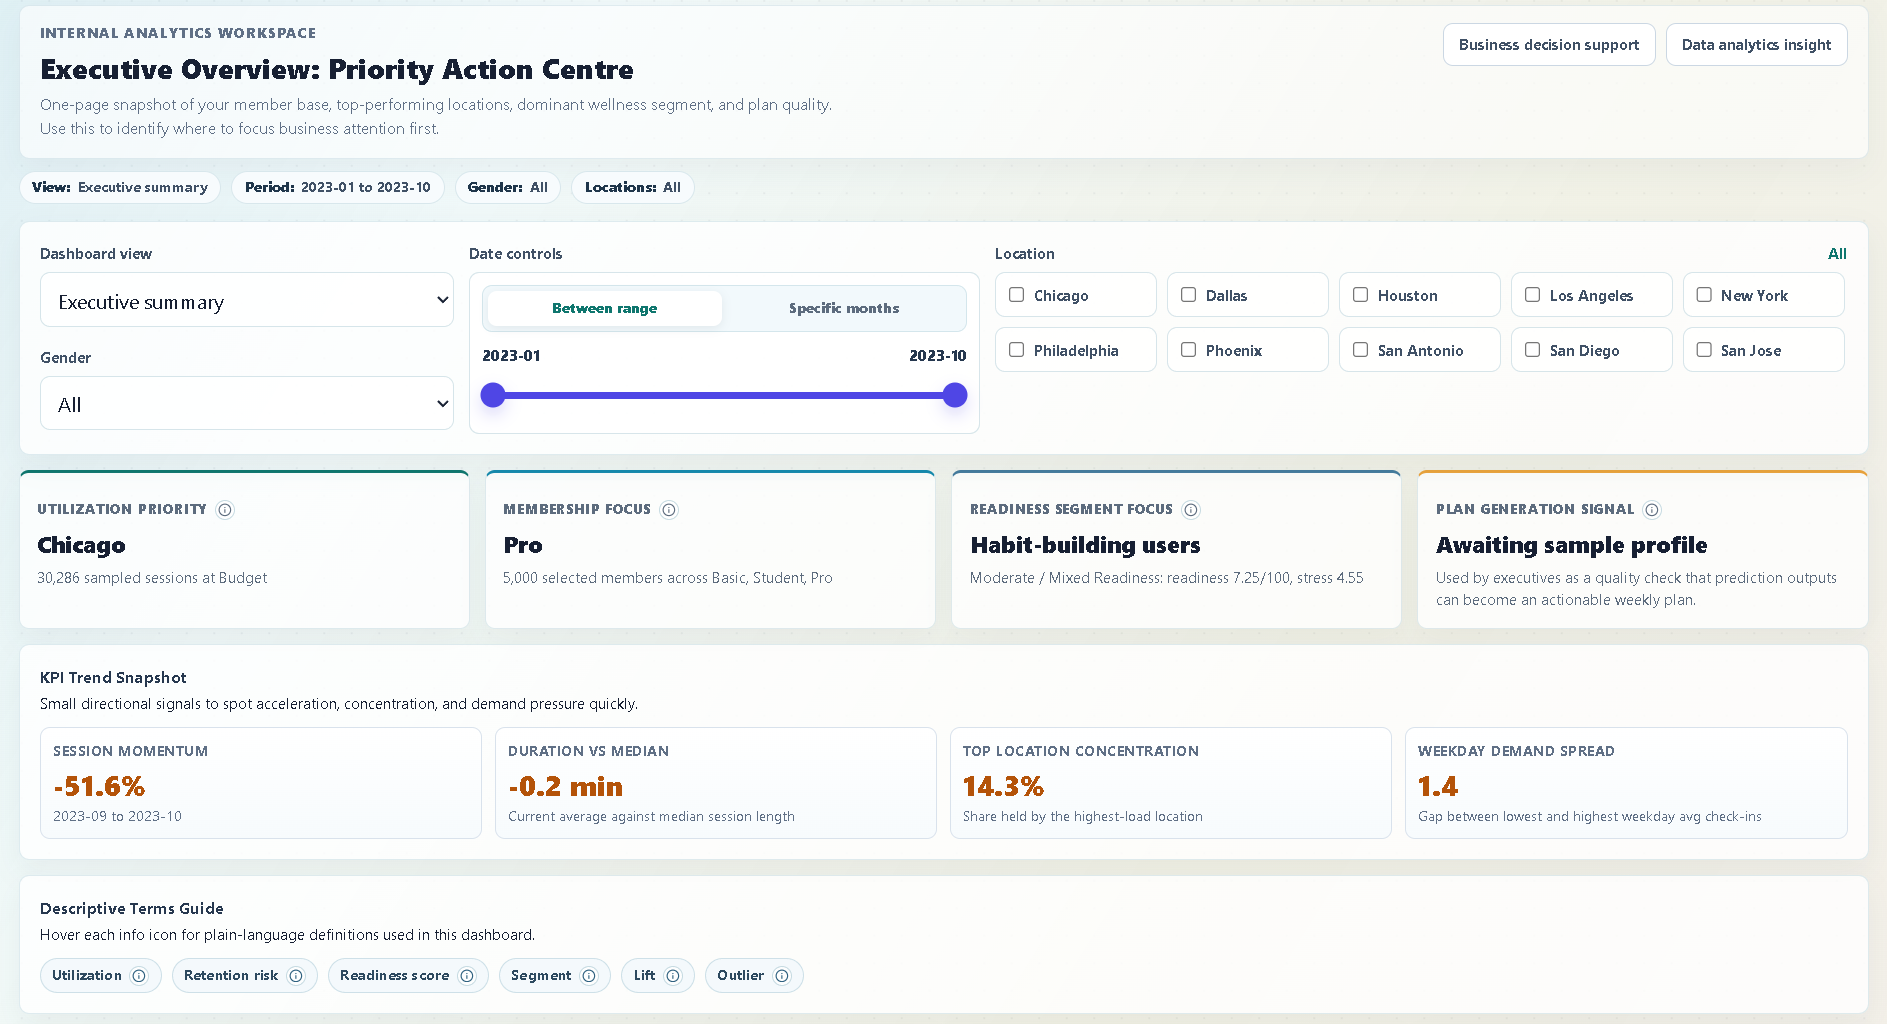
\includegraphics[width=0.92\linewidth]{figures/Dashboard Figure/Executive Summary before A.png}
    \caption{Executive summary before the final layout redesign.}
    \label{fig:chapter4_exec_before}
\end{figure}

\begin{figure}[H]
    \centering
    \begin{subfigure}[t]{0.92\linewidth}
        \centering
        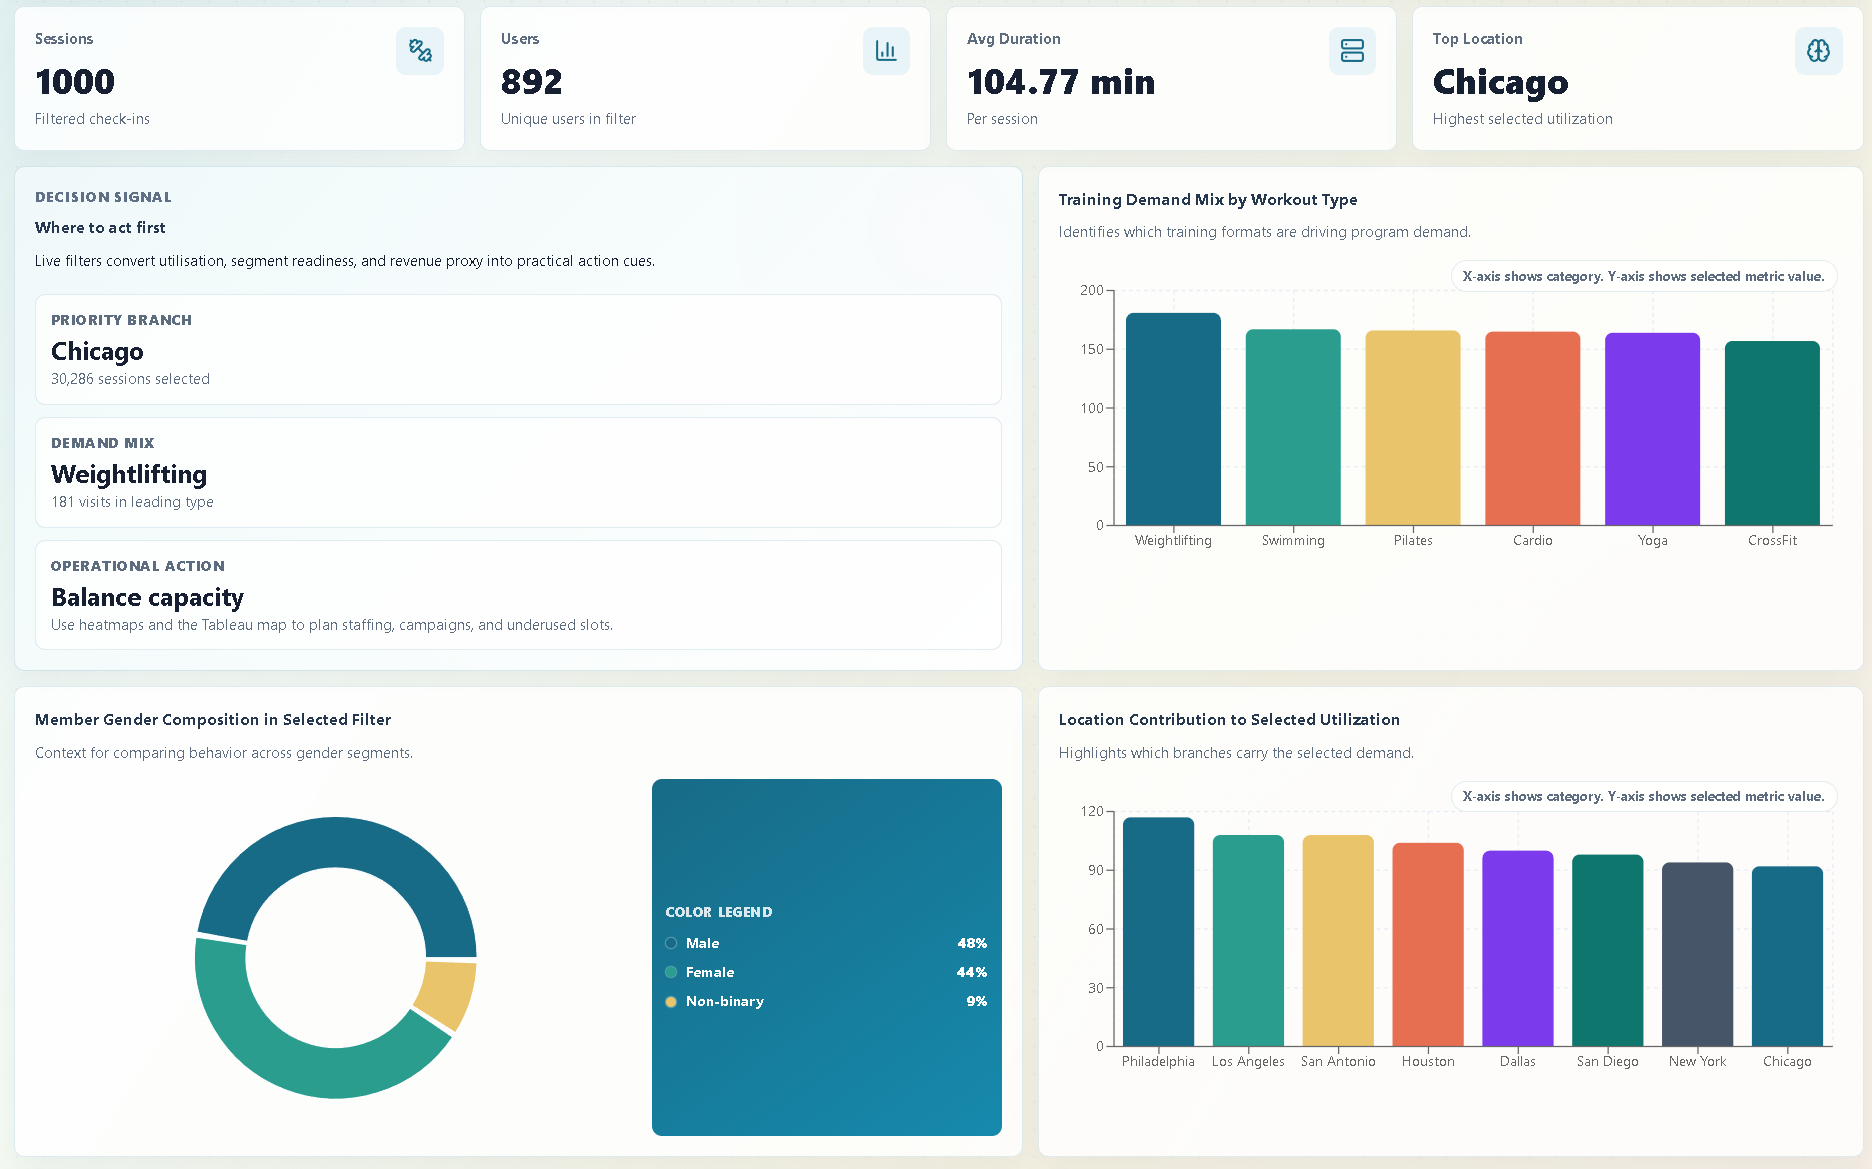
\includegraphics[width=\linewidth]{figures/Dashboard Figure/Executive Summary A.png}
        \caption{Executive summary, section A}
    \end{subfigure}\\[3pt]
    \begin{subfigure}[t]{0.92\linewidth}
        \centering
        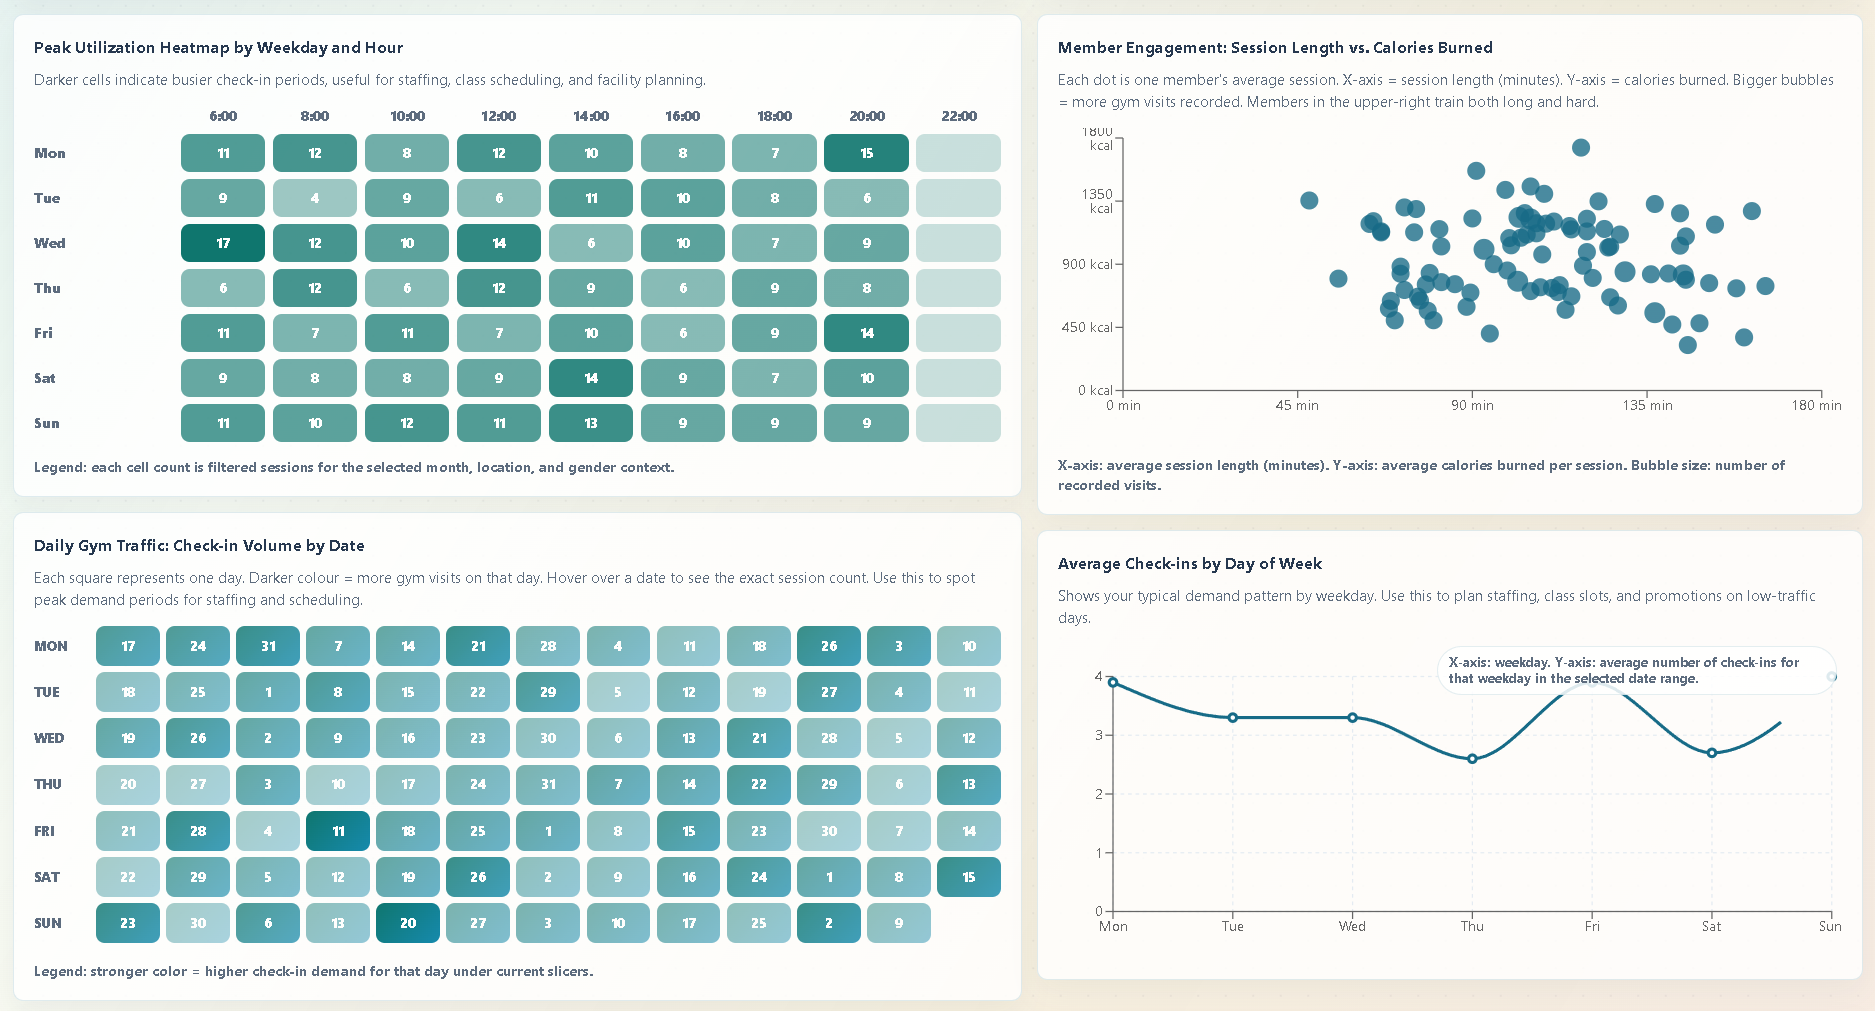
\includegraphics[width=\linewidth]{figures/Dashboard Figure/Executive Summary B.png}
        \caption{Executive summary, section B}
    \end{subfigure}
    \caption{Final executive summary dashboard.}
    \label{fig:chapter4_exec_summary}
\end{figure}

The important result from the executive summary is that it reduces the analysis path from several separate datasets into one decision surface. Branch performance, time filtering, segment mix, and action signals are visible together, so managers can compare utilization and estimated revenue share before making staffing or campaign decisions.

\begin{figure}[H]
    \centering
    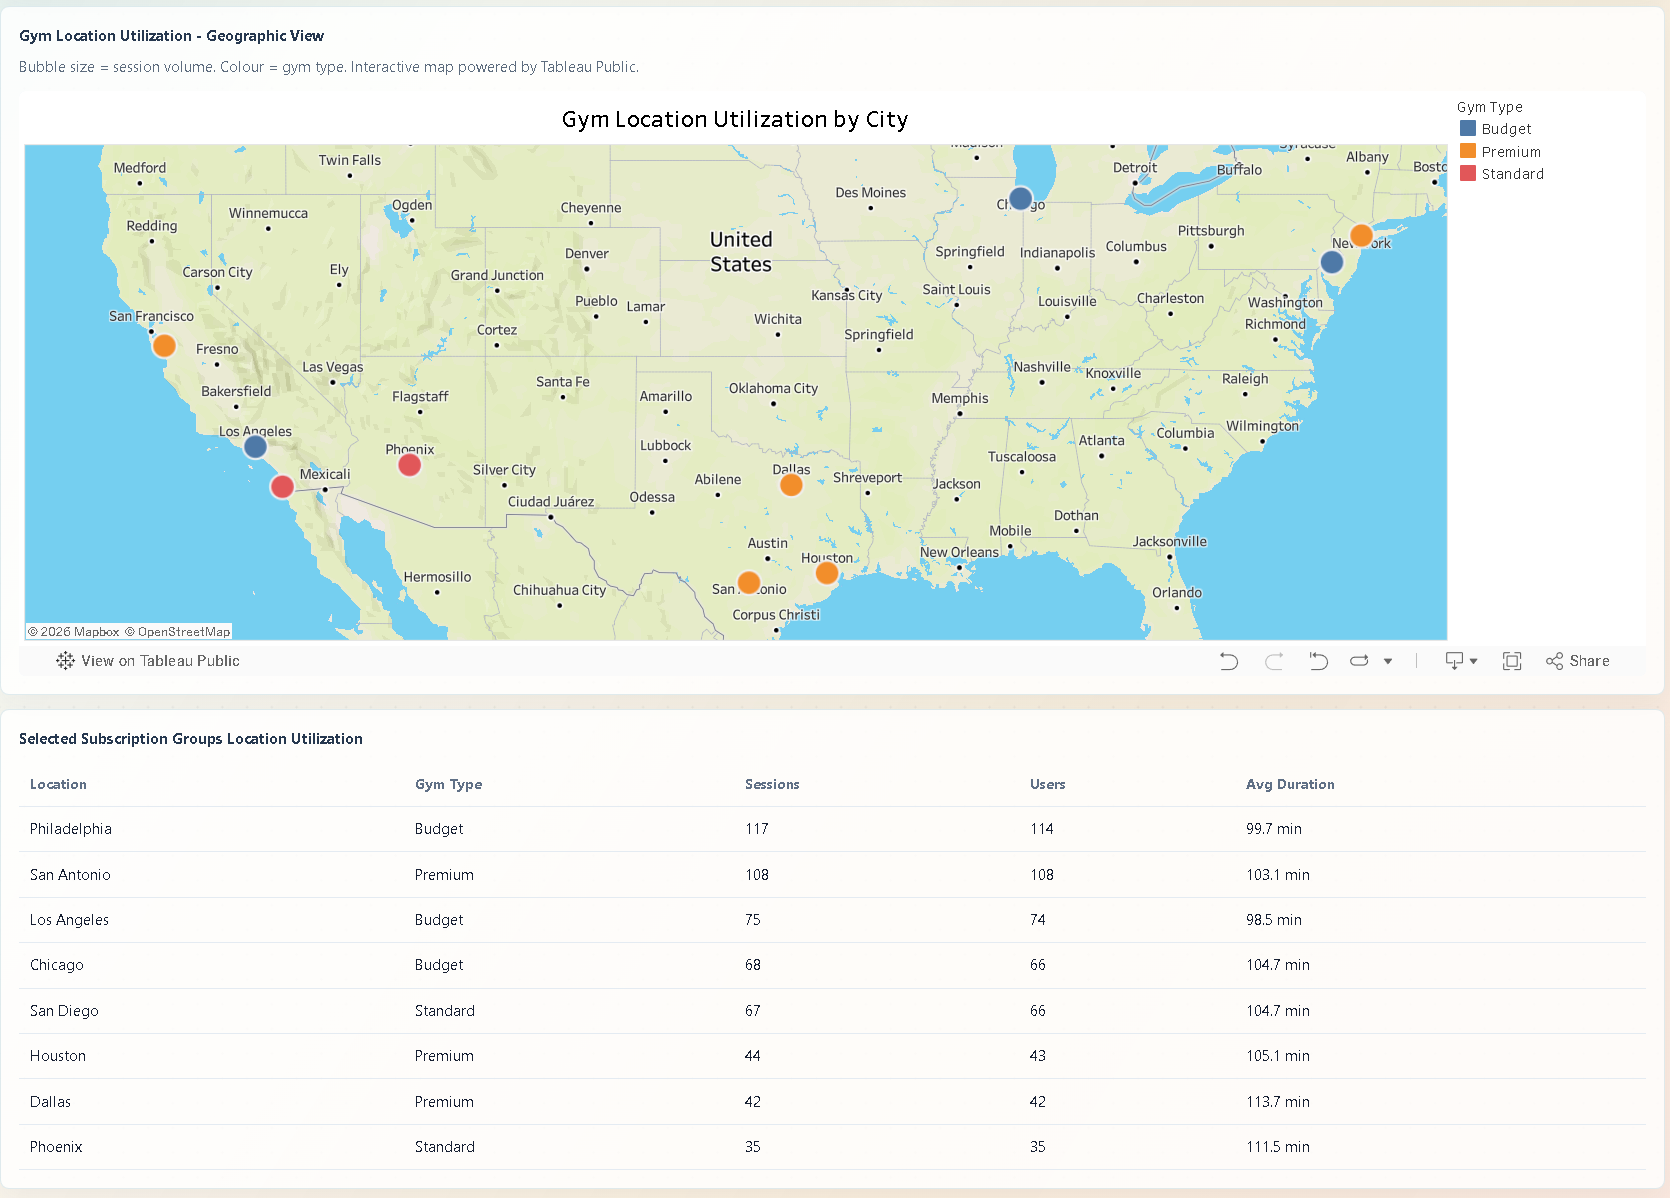
\includegraphics[width=0.92\linewidth]{figures/tableau_monitor_map_embed v.2.png}
    \caption{Tableau gym-location map embedded beside branch utilization panels.}
    \label{fig:chapter4_tableau_map}
\end{figure}

The embedded Tableau map is the geospatial complement to the executive summary's tables and bars: bubble size encodes session volume and colour encodes gym type, so a manager can see at a glance which branches combine high volume with a specific facility type before drilling into the utilization or revenue-signal panels. Table~\ref{tab:chapter4_business_visual_action} lists this map alongside the executive summary as the recommended pairing for the branch-staffing and campaign-priority decision.

Geographically, utilization does not track gym tier in a simple way. Philadelphia, a Budget-tier location, leads the mapped locations with 117 sessions and 114 users, ahead of San Antonio (Premium, 108 sessions) and Los Angeles (Budget, 75 sessions); Chicago and San Diego sit in the middle of the range (68 and 67 sessions), while Houston, Dallas, and Phoenix trail at 35--44 sessions despite two of the three being Premium locations. Average session duration is comparatively stable across the map (98.5--113.7 minutes), so the map's main decision signal is volume concentration rather than visit length: Philadelphia and San Antonio alone account for a disproportionate share of the mapped session volume, which is the kind of branch-level concentration the utilization-priority decision in Table~\ref{tab:chapter4_business_visual_action} is designed to surface.

\begin{figure}[H]
    \centering
    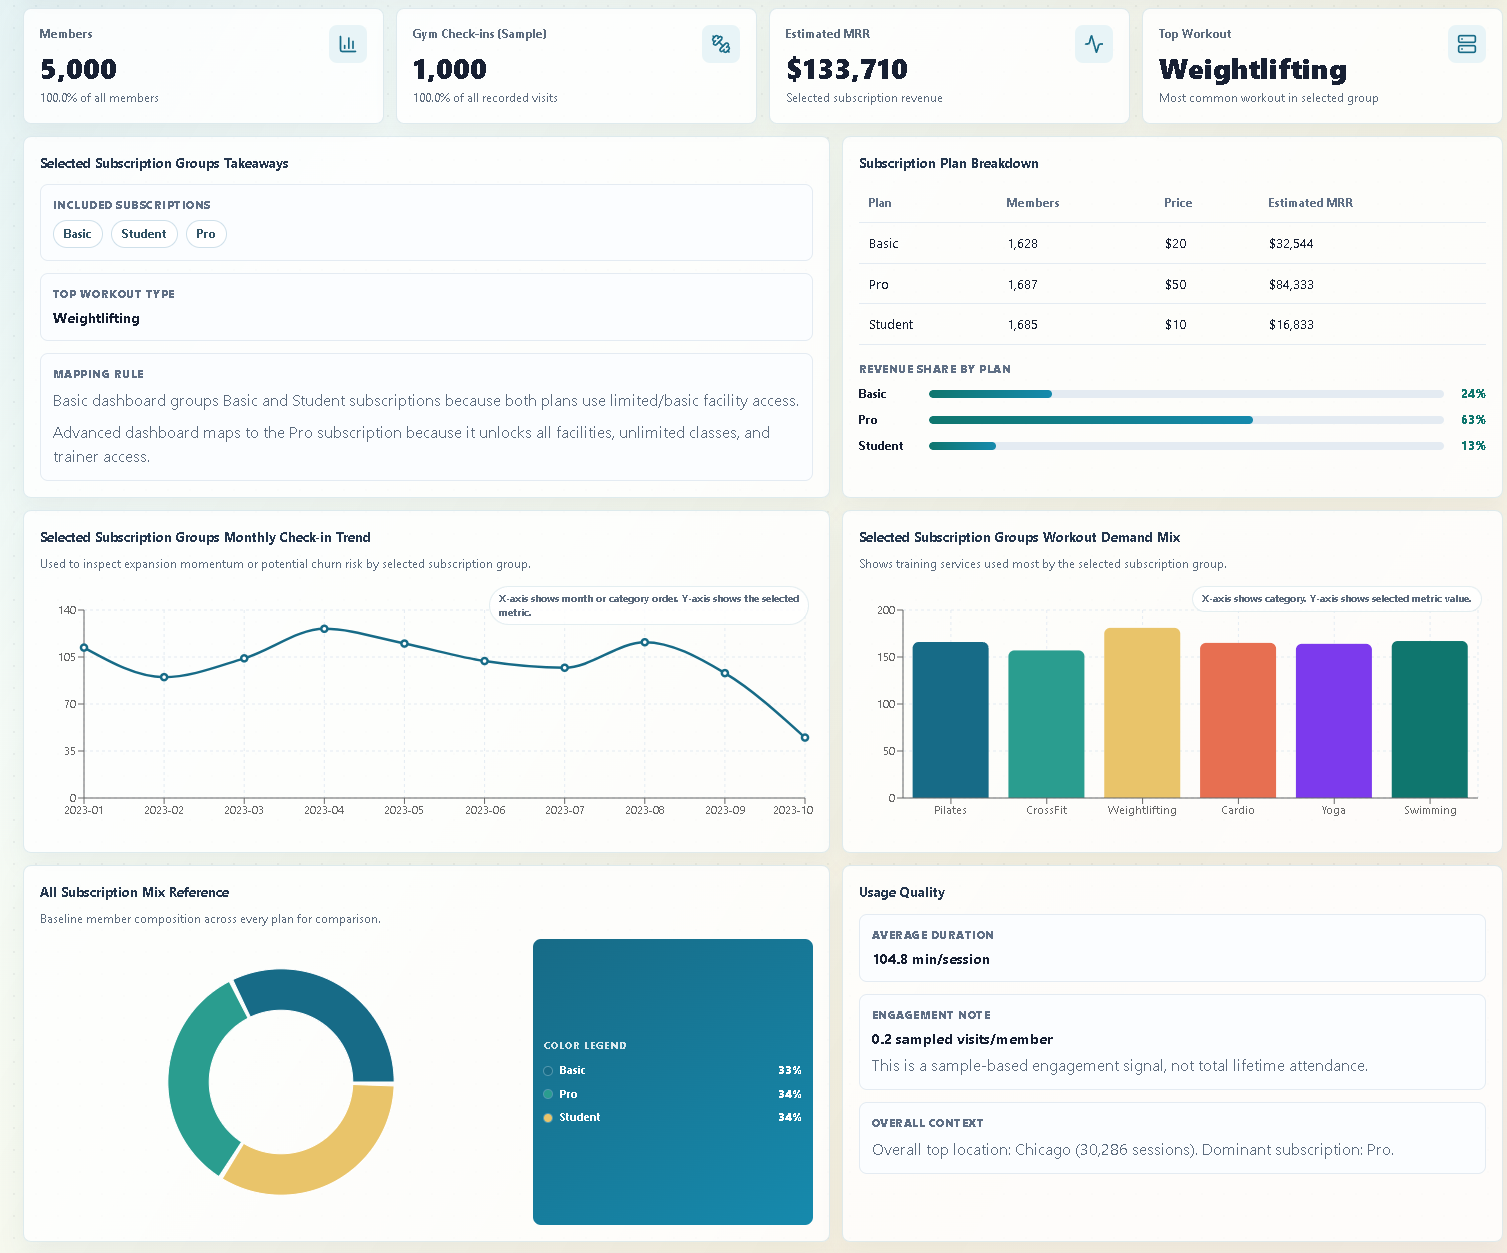
\includegraphics[width=0.92\linewidth]{figures/Dashboard Figure/Membership Utilisation and Revenue Signals A.png}
    \caption{Membership utilisation and revenue signals.}
    \label{fig:chapter4_membership_revenue}
\end{figure}

The membership utilisation and revenue view answers whether high activity also corresponds with high estimated revenue share. This matters because an overloaded branch and a high-value branch may require different responses: one may need capacity planning, while the other may justify retention or upsell campaigns.

\begin{figure}[H]
    \centering
    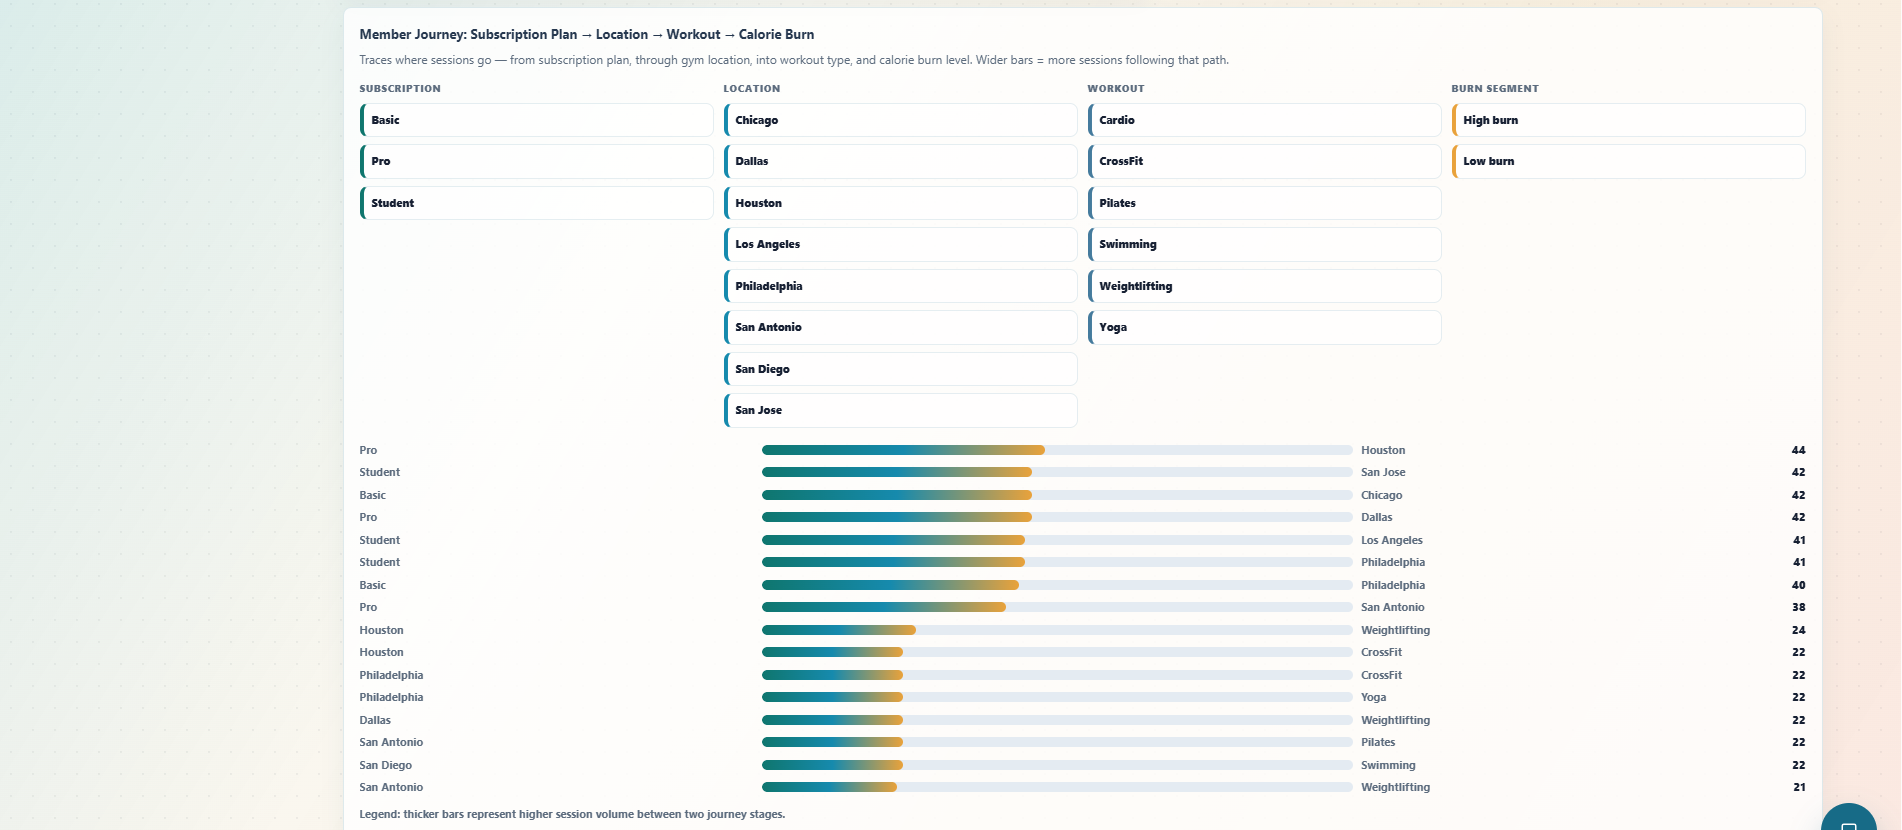
\includegraphics[width=0.95\linewidth]{figures/Dashboard Figure/Executive Dashboard Sankey.png}
    \caption{Member journey: subscription plan to location to workout to calorie-burn segment.}
    \label{fig:chapter4_journey_sankey}
\end{figure}

The member journey view is the executive dashboard's most direct answer to the subscription-cohort question in Table~\ref{tab:chapter4_business_visual_action}: which cohorts carry retention risk or upsell potential. Read left to right, it traces sessions from subscription plan, through gym location, into workout type, and finally into a High-burn or Low-burn segment, so a manager can see not just which plan is largest but where its sessions actually go. In the captured filter, Pro-Houston, Student-San Jose, Basic-Chicago, and Pro-Dallas carry the heaviest plan-to-location volume (38--44 sessions each), while the location-to-workout stage shows Weightlifting and CrossFit absorbing most of the downstream traffic across Houston, Philadelphia, Dallas, and San Antonio. Because the flow is built from live filtered data rather than a static assumption, it lets an executive test a specific hypothesis (for example, whether the Pro cohort is concentrated in a small number of locations) instead of inferring it indirectly from separate tables.

\begin{figure}[H]
    \centering
    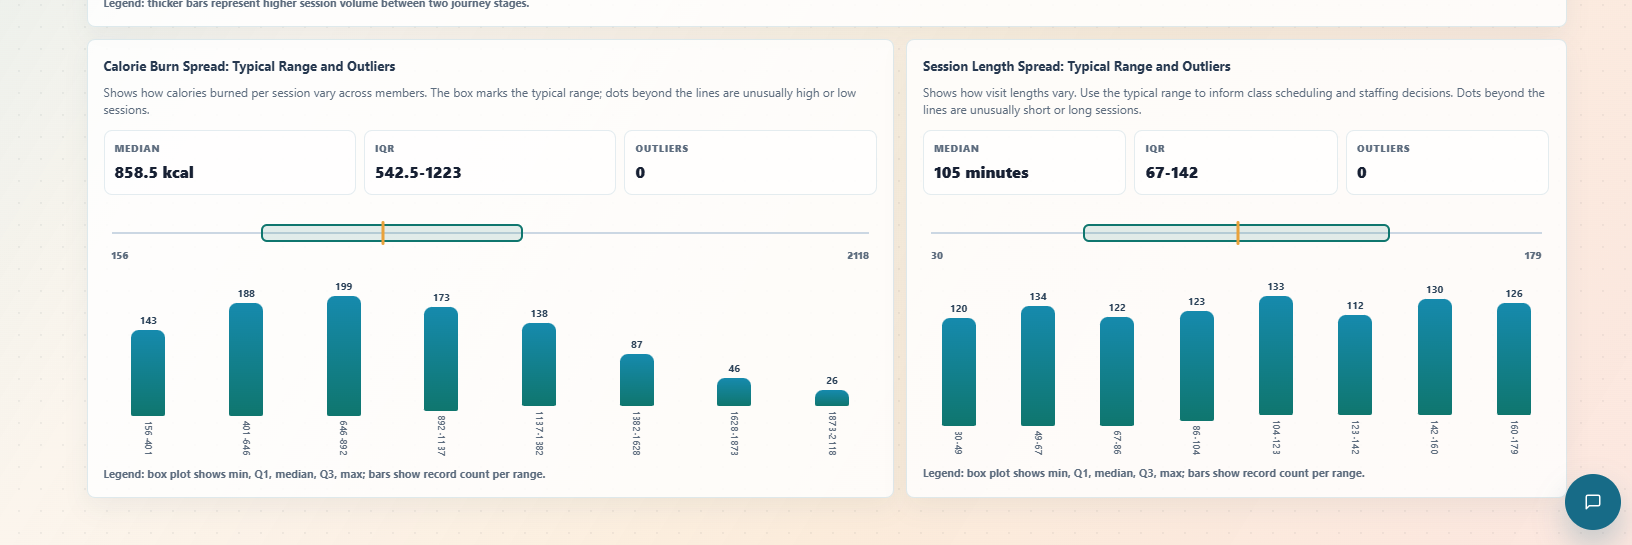
\includegraphics[width=0.95\linewidth]{figures/Dashboard Figure/Executive Dashboard Distributions.png}
    \caption{Calorie-burn and session-length distributions for the selected filter.}
    \label{fig:chapter4_distributions}
\end{figure}

The two distribution panels quantify how much variation sits behind the averages shown elsewhere on the executive summary. Calorie burn per session has a median of 858.5 kcal with an interquartile range of 542.5--1223 kcal, and session length has a median of 105 minutes with an interquartile range of 67--142 minutes; in this filtered sample neither distribution flags a formal outlier, but both are visibly right-skewed, with a longer tail of high-burn, long-duration sessions than short ones. This matters for the same retention and capacity decisions as the Sankey panel above: a branch or cohort whose typical range is wide is less predictable to staff and plan around than one whose sessions cluster tightly, so these box plots are the evidence an executive would check before committing to a class-scheduling or capacity change suggested by the utilization views.

\subsection{Lifestyle Segment Result}
\label{sec:lifestyle_segment_result}

The lifestyle segment view connects descriptive member profiles with readiness. It is designed for the question of which lifestyle segments have the largest member share, the lowest readiness, and the clearest need for intervention.

\begin{figure}[H]
    \centering
    \begin{subfigure}[t]{0.6\linewidth}
        \centering
        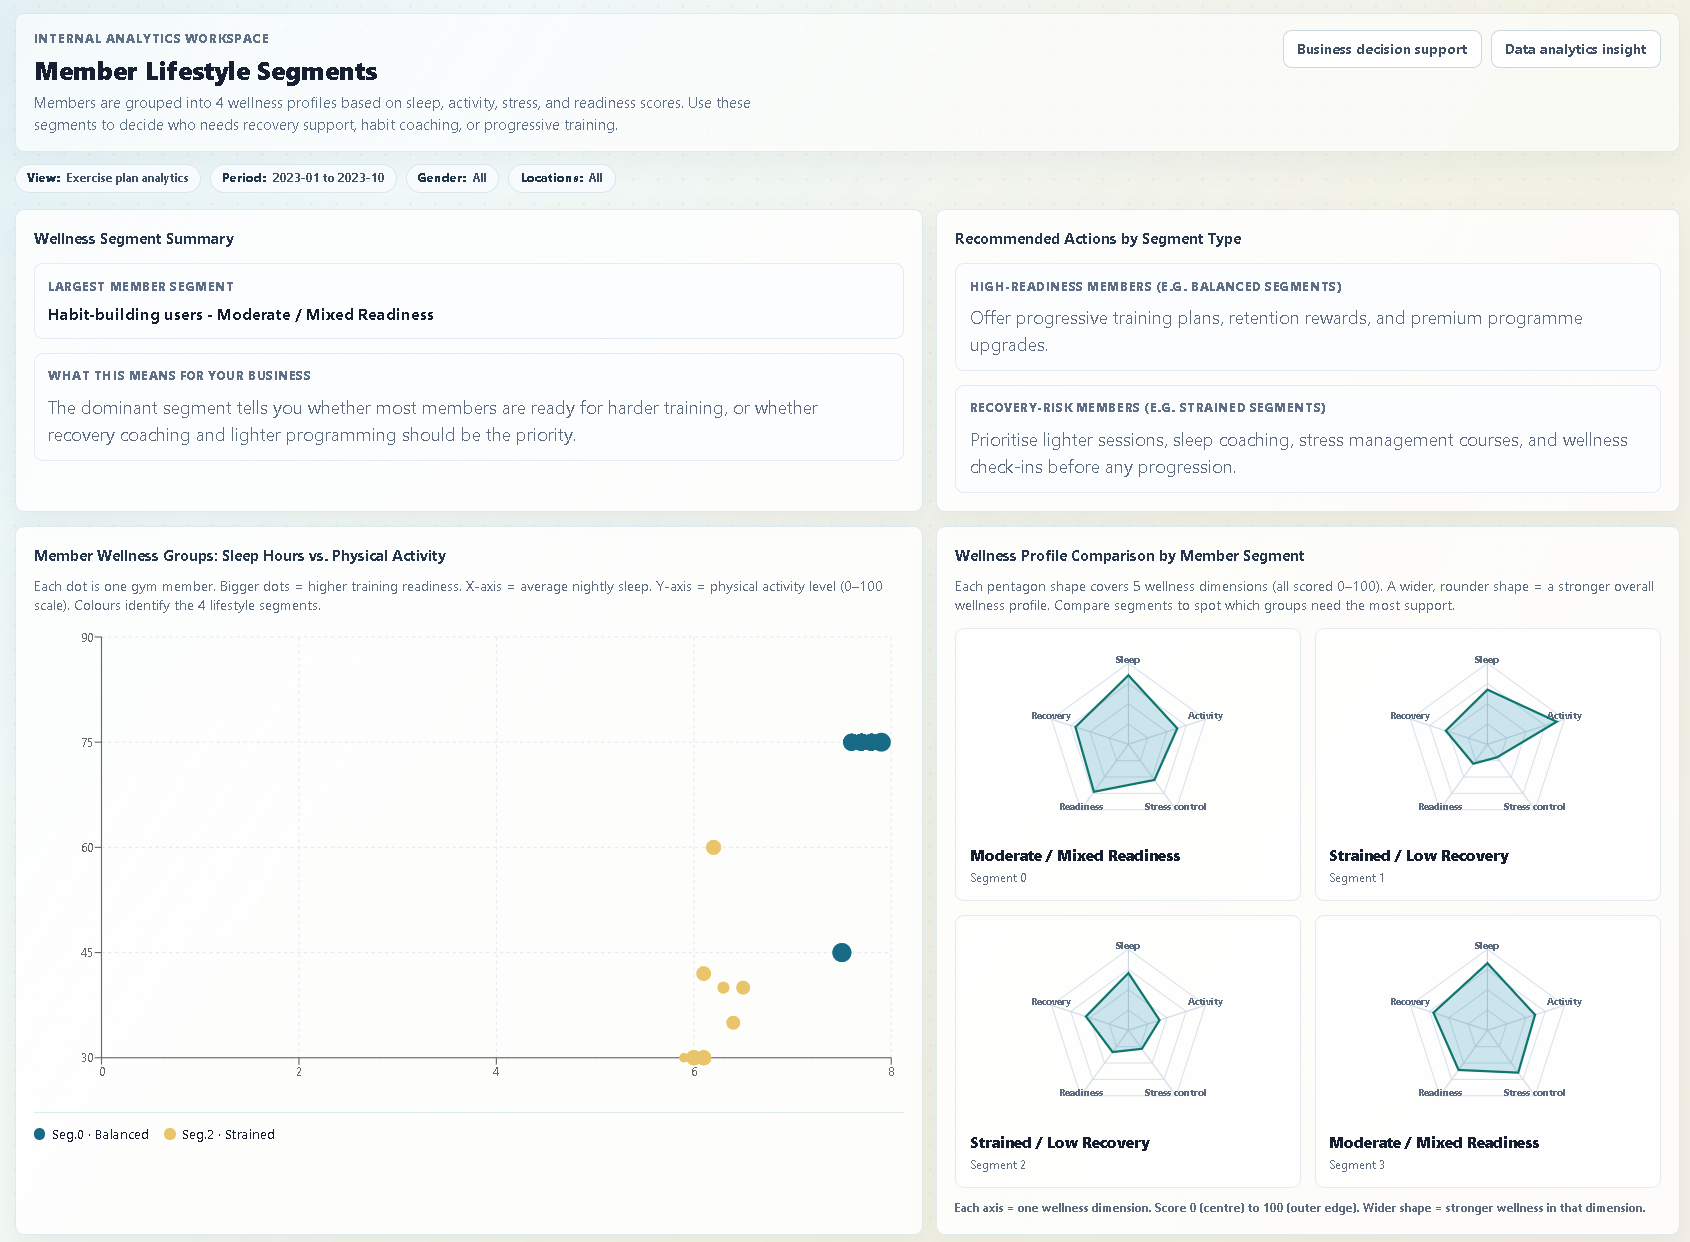
\includegraphics[width=\linewidth]{figures/Dashboard Figure/Member Lifestyle Segments A.png}
        \caption{Segment overview}
    \end{subfigure}\\[3pt]
    \begin{subfigure}[t]{0.6\linewidth}
        \centering
        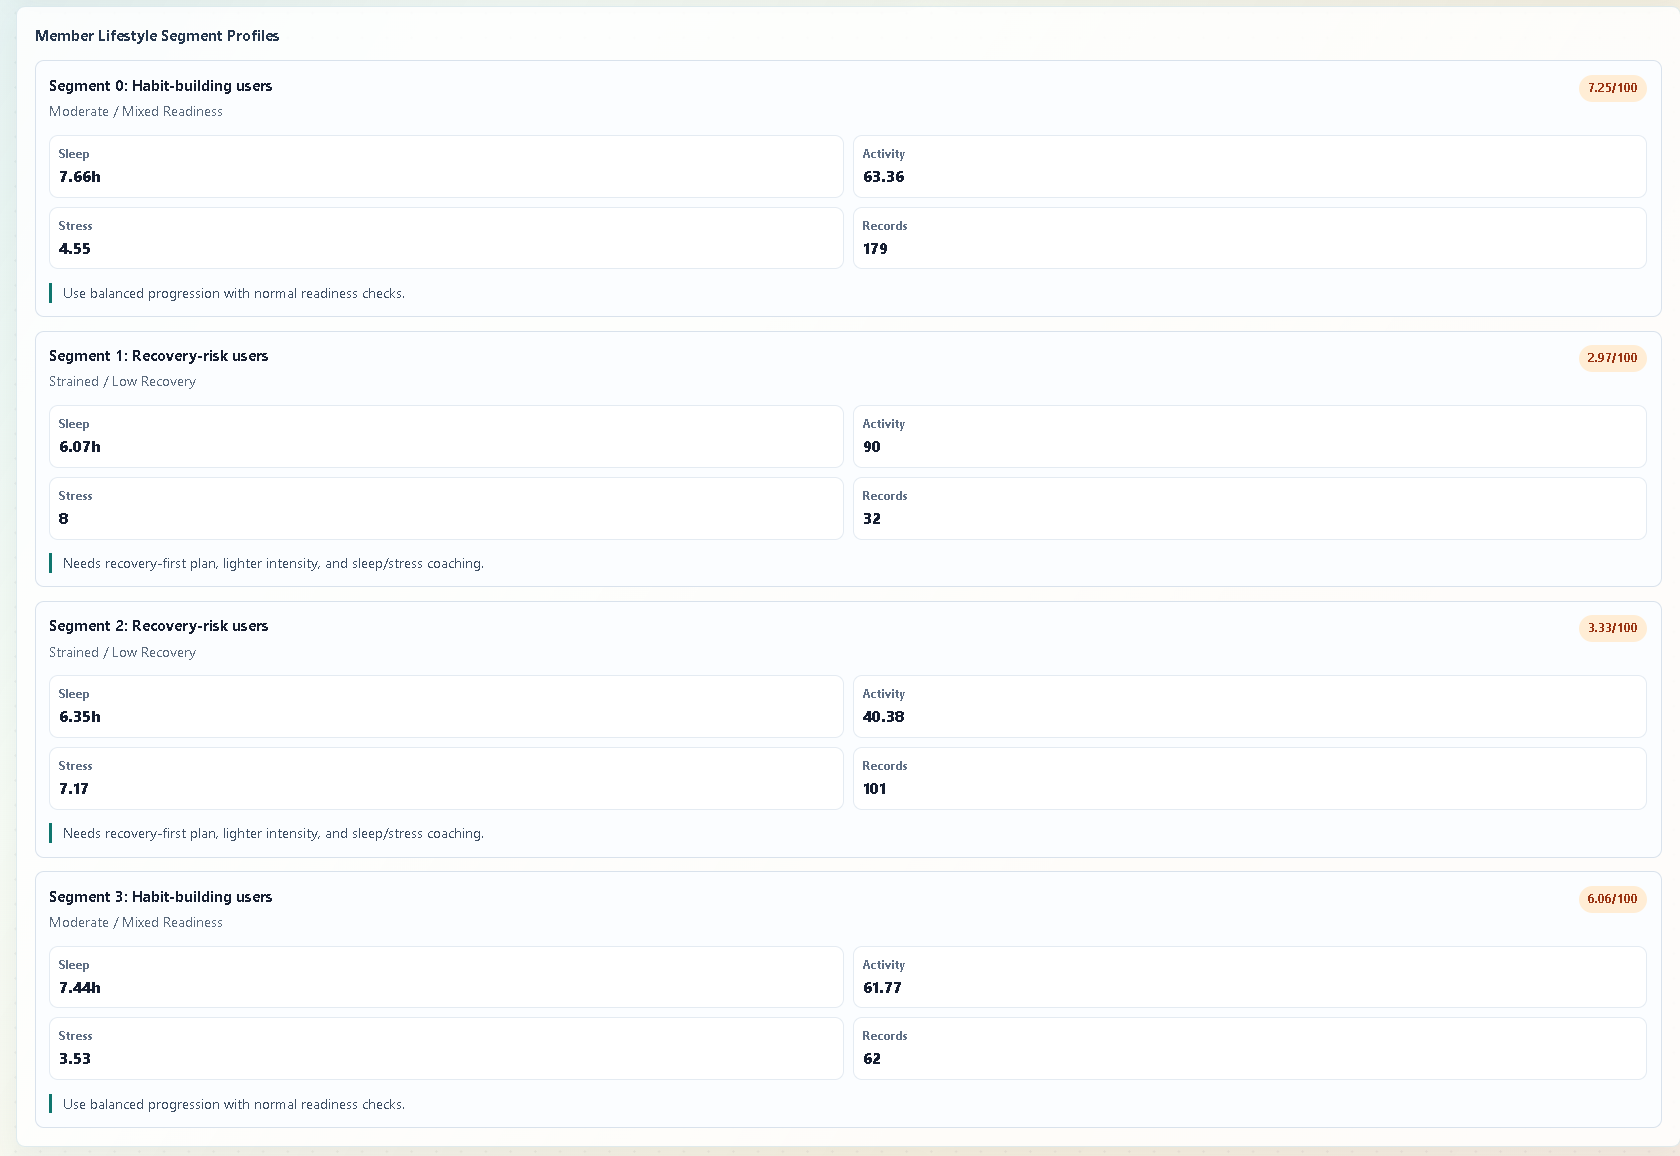
\includegraphics[width=\linewidth]{figures/Dashboard Figure/Member Lifestyle Segments B.png}
        \caption{Segment comparison}
    \end{subfigure}\\[3pt]
    \begin{subfigure}[t]{0.6\linewidth}
        \centering
        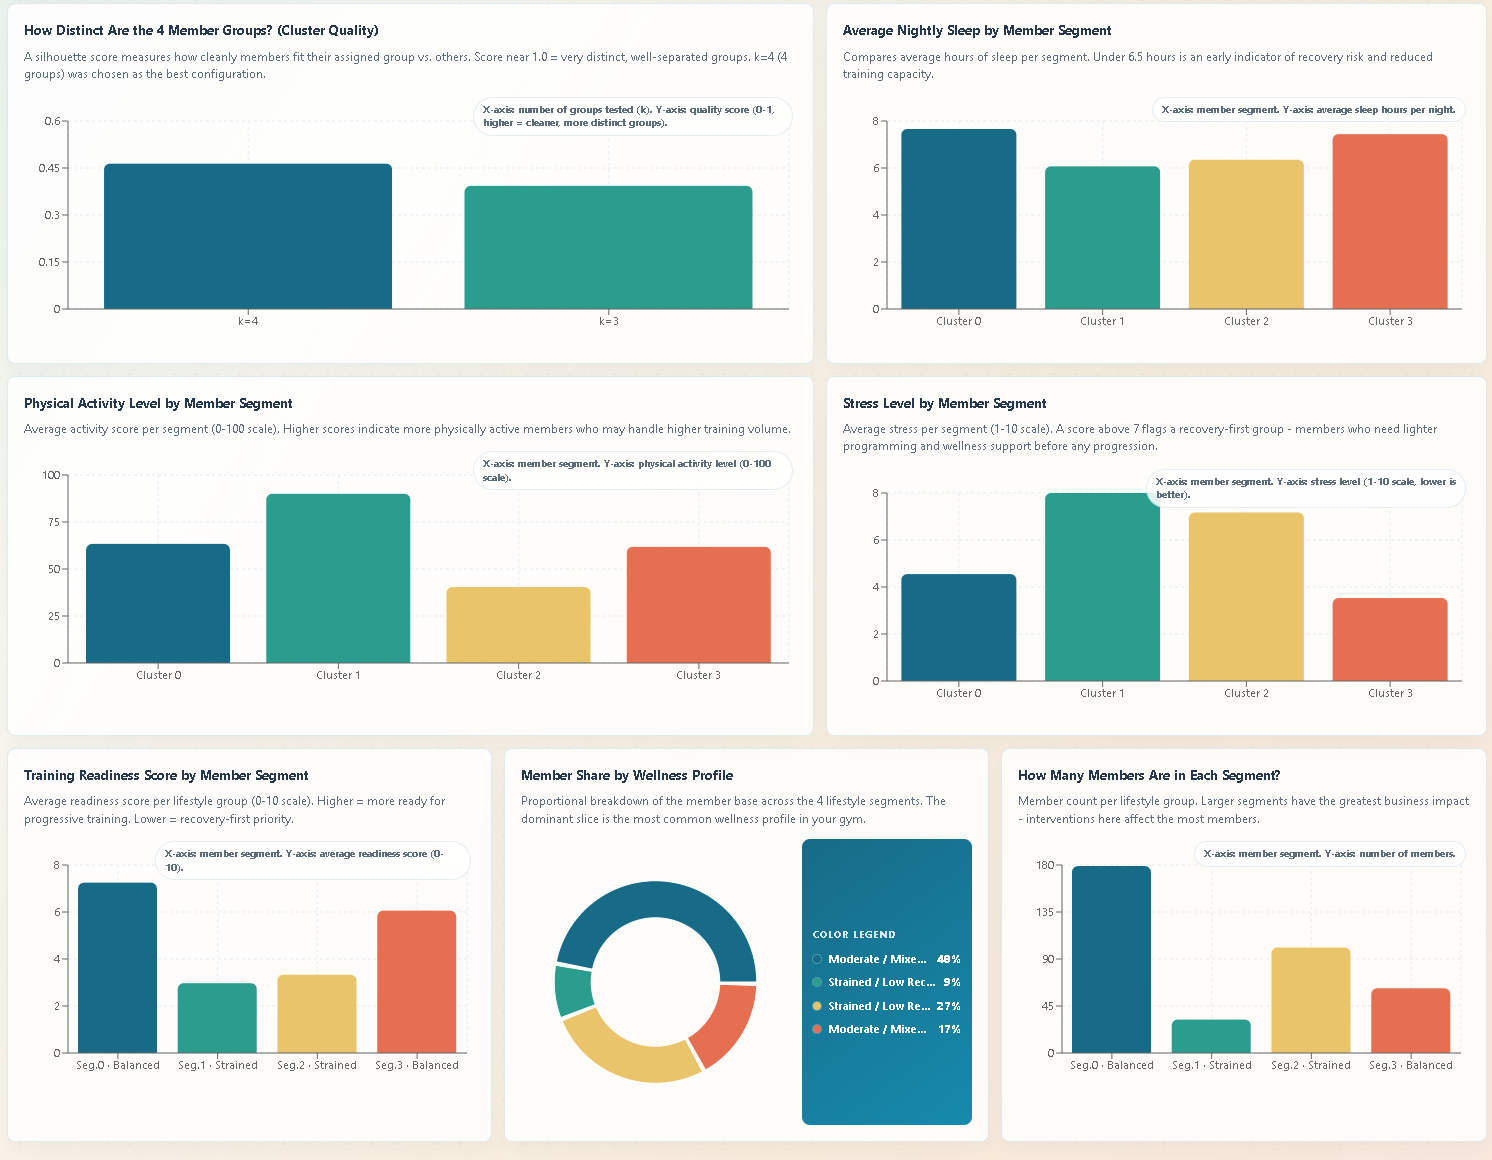
\includegraphics[width=\linewidth]{figures/Dashboard Figure/Member Lifestyle Segments C.png}
        \caption{Segment detail}
    \end{subfigure}
    \caption{Member lifestyle segment dashboard.}
    \label{fig:chapter4_lifestyle_segments}
\end{figure}

The important result is that lifestyle segments give the dashboard a bridge between business monitoring and personalized recommendation. A low-readiness segment can be treated as a candidate for recovery-focused messaging, while a high-readiness and high-engagement segment can be treated as a candidate for progression or upsell.

\subsection{Exercise Plan and User Result}

The user-facing dashboard translates model outputs into practical plan guidance. It shows the profile and readiness inputs before plan generation, then displays plan analytics, member profile context, and nutrition context. This supports the user questions about which inputs influence readiness, what predicted intensity means, and what to track weekly.

\begin{figure}[H]
    \centering
    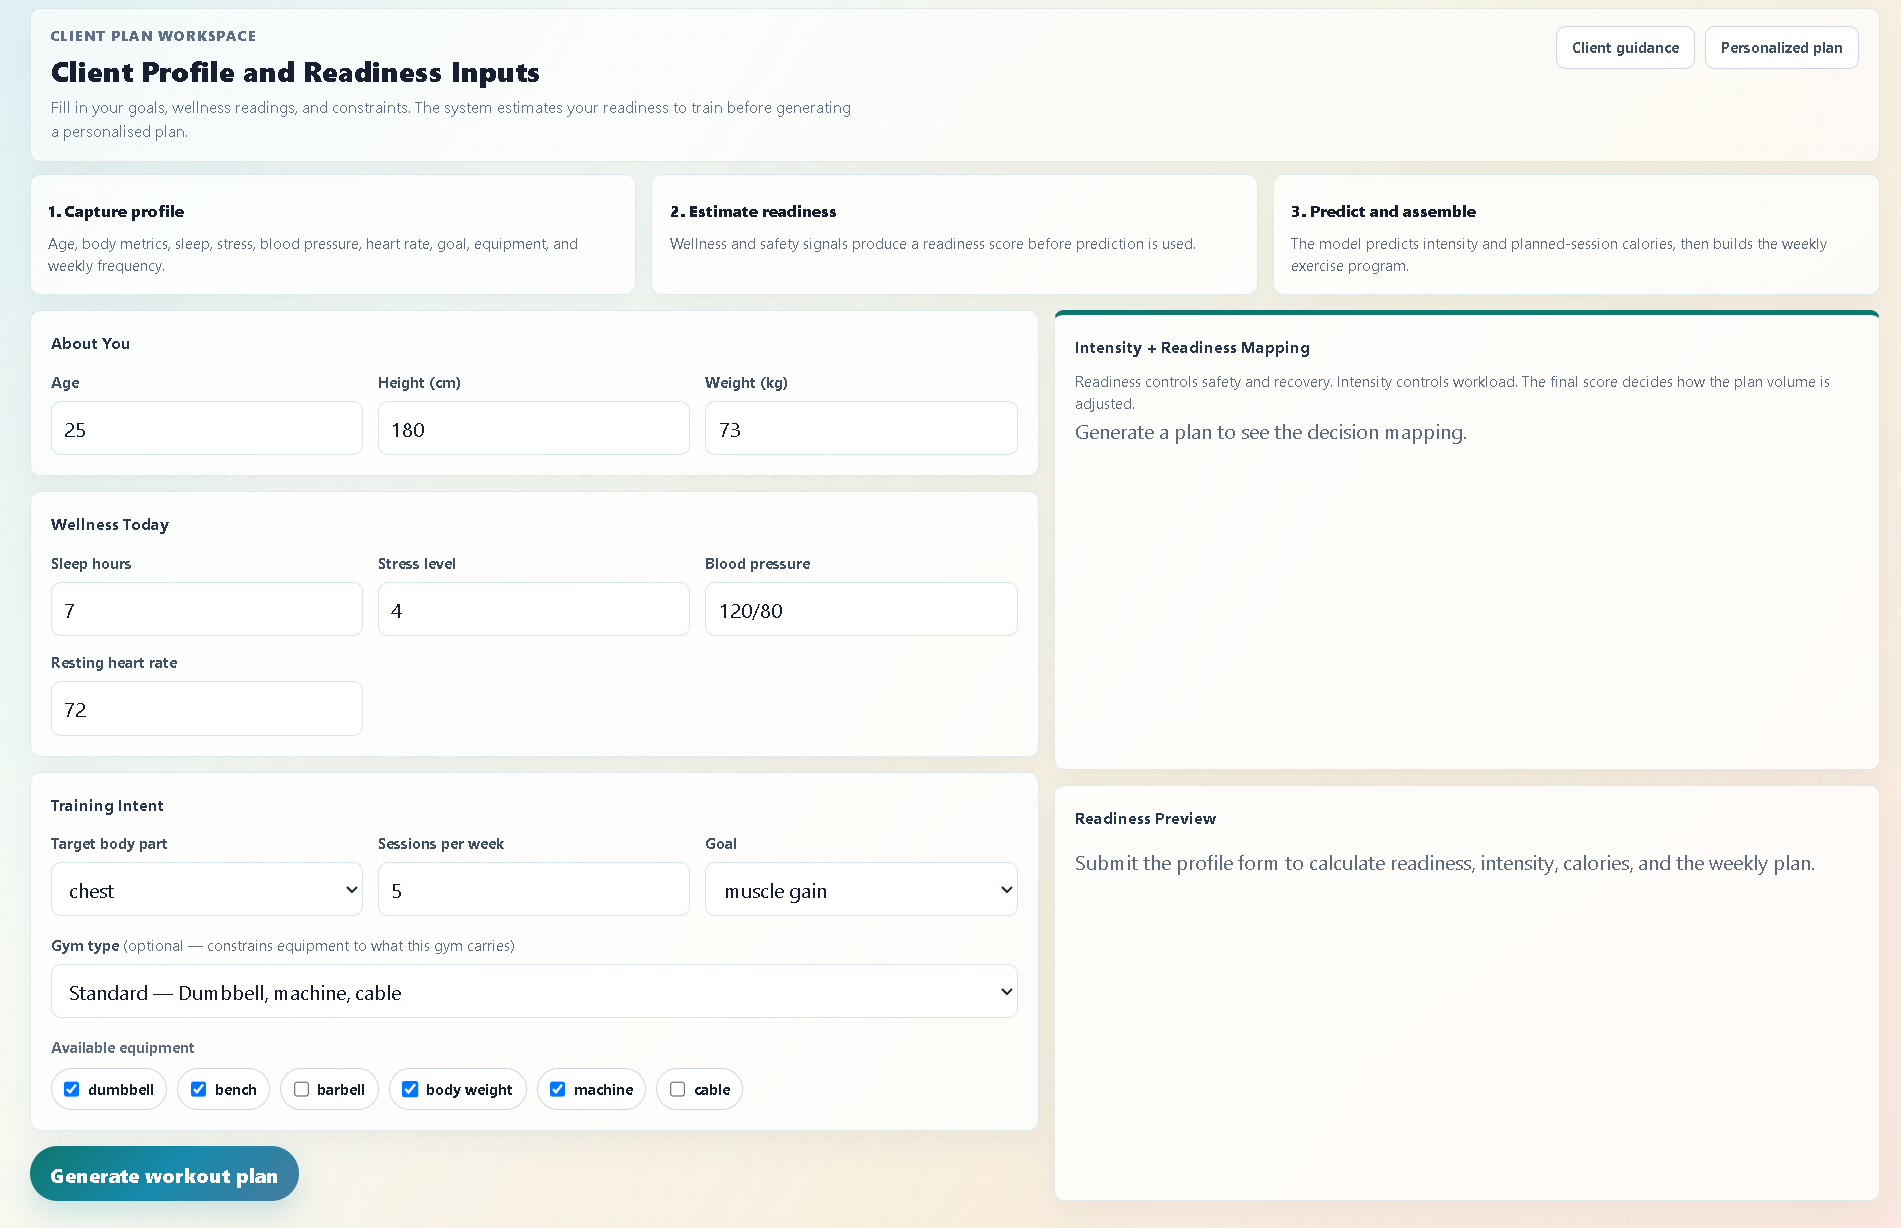
\includegraphics[width=0.92\linewidth]{figures/Dashboard Figure/Client Profile and Readiness Inputs Before Generated.png}
    \caption{Client profile and readiness inputs before plan generation.}
    \label{fig:chapter4_client_inputs}
\end{figure}

The profile input result shows that the plan is not generated from a single goal field. It incorporates readiness-related inputs such as sleep, stress, activity, constraints, and body context, which are then converted into intensity and plan recommendations.

\begin{figure}[H]
    \centering
    \begin{subfigure}[t]{0.85\linewidth}
        \centering
        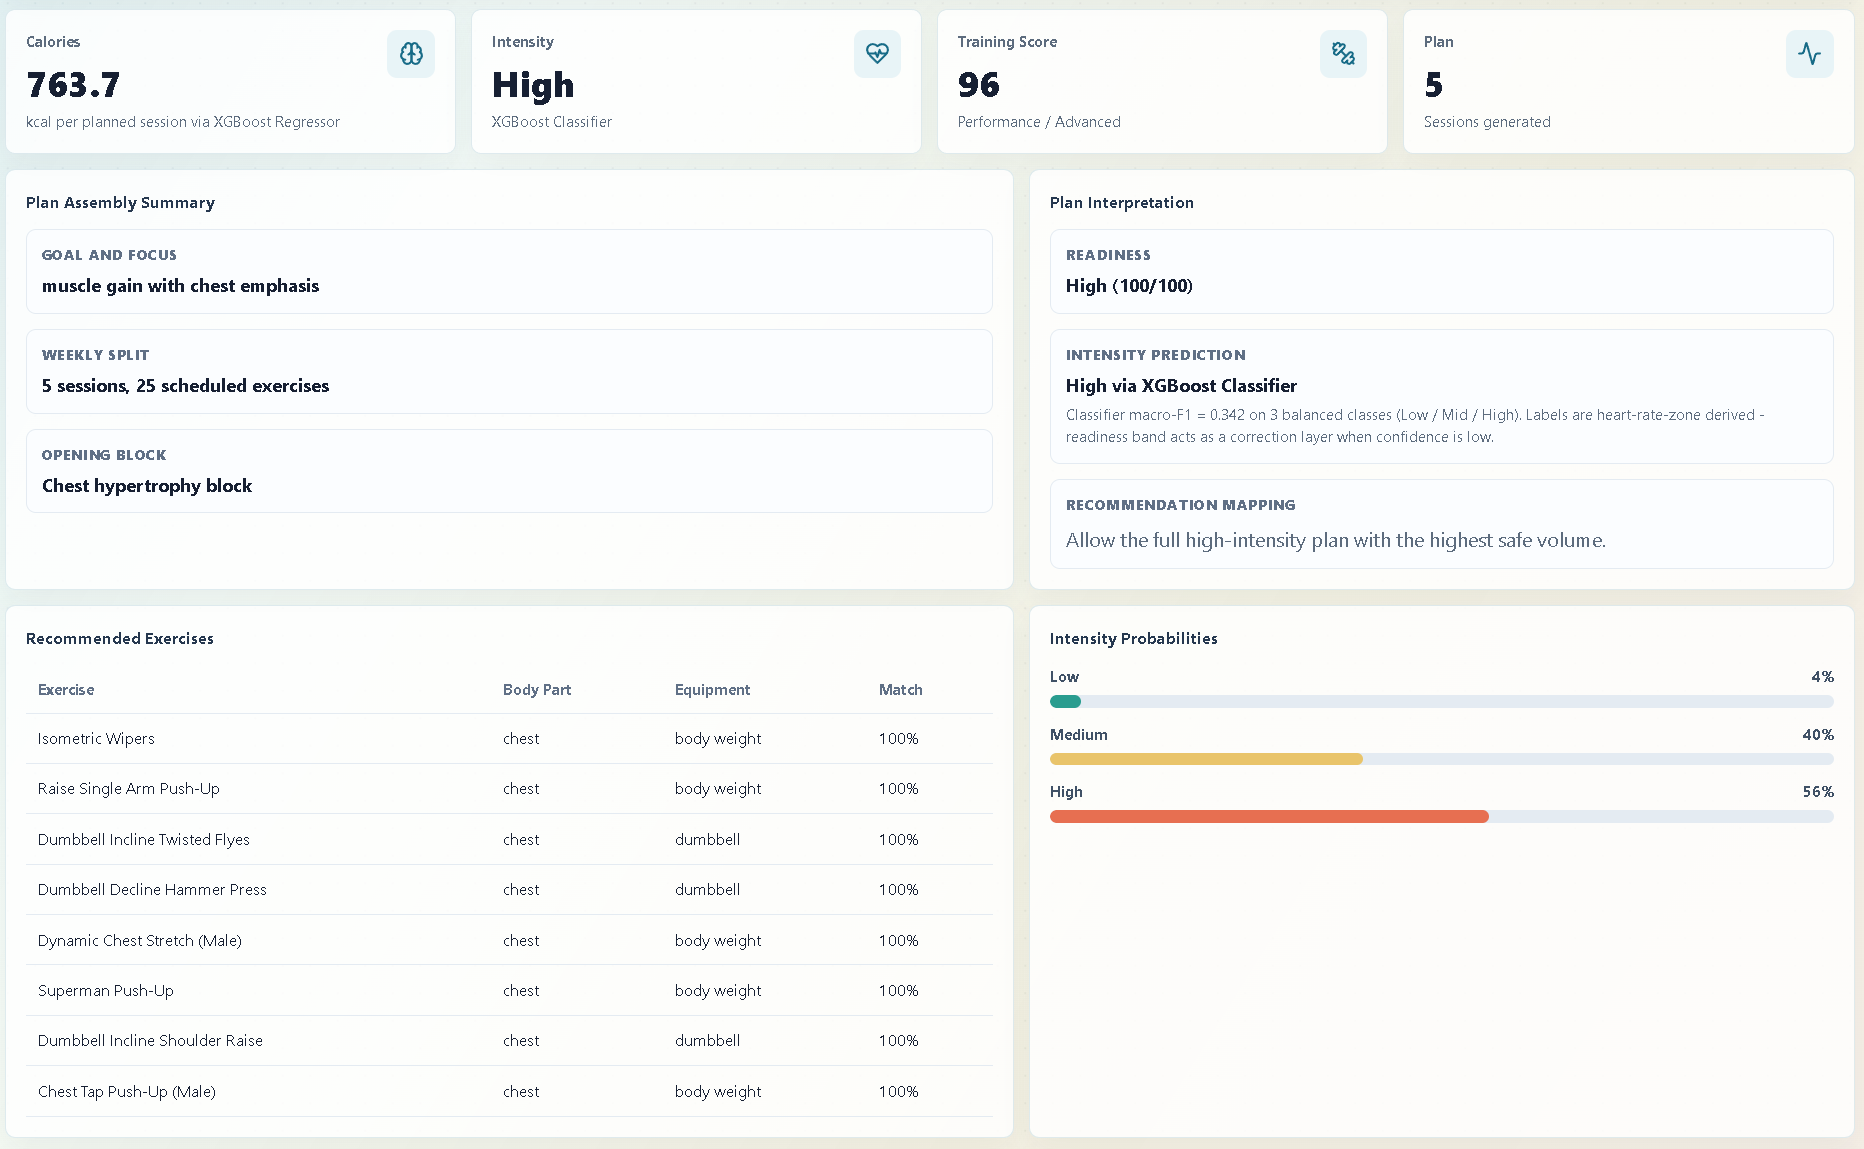
\includegraphics[width=\linewidth]{figures/Dashboard Figure/Client Profile and Readiness Inputs Before Plan.png}
        \caption{Inputs before plan generation}
    \end{subfigure}\\[3pt]
    \begin{subfigure}[t]{0.85\linewidth}
        \centering
        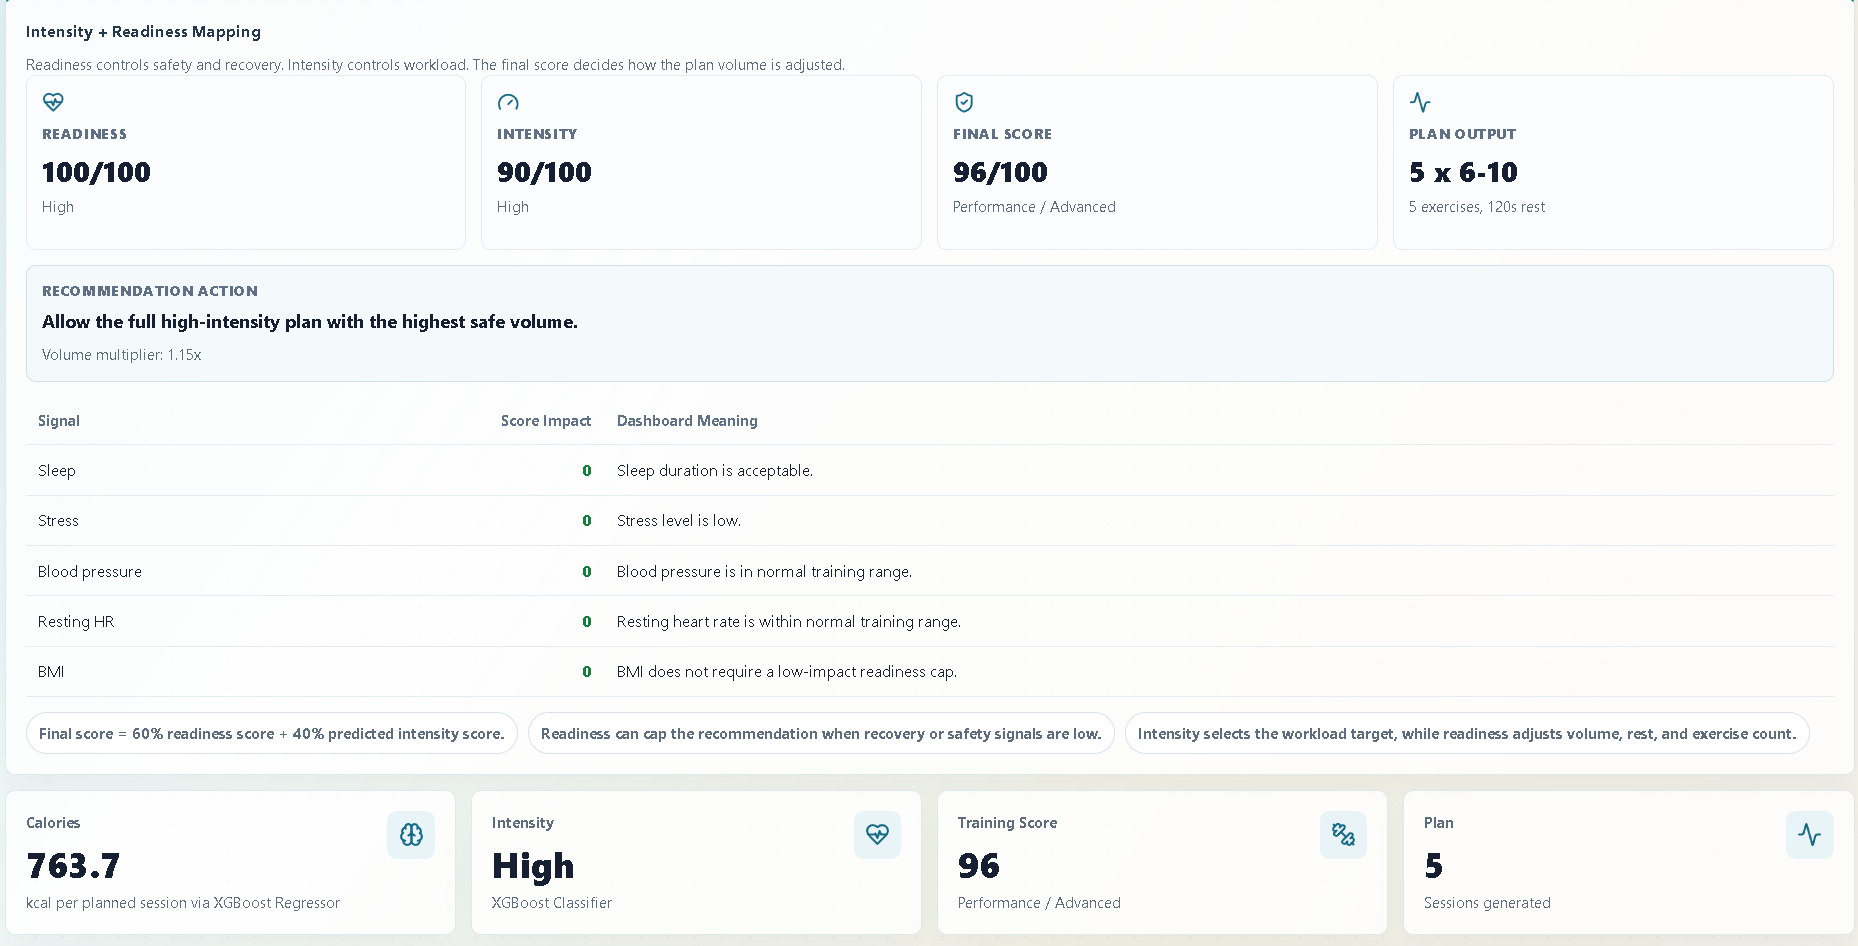
\includegraphics[width=\linewidth]{figures/Dashboard Figure/Client Profile and Readiness Inputs Before Result.png}
        \caption{Initial readiness result}
    \end{subfigure}
    \caption{Readiness-to-result workflow.}
    \label{fig:chapter4_client_profile_workflow_a}
\end{figure}

\begin{figure}[H]
    \centering
    \begin{subfigure}[t]{0.85\linewidth}
        \centering
        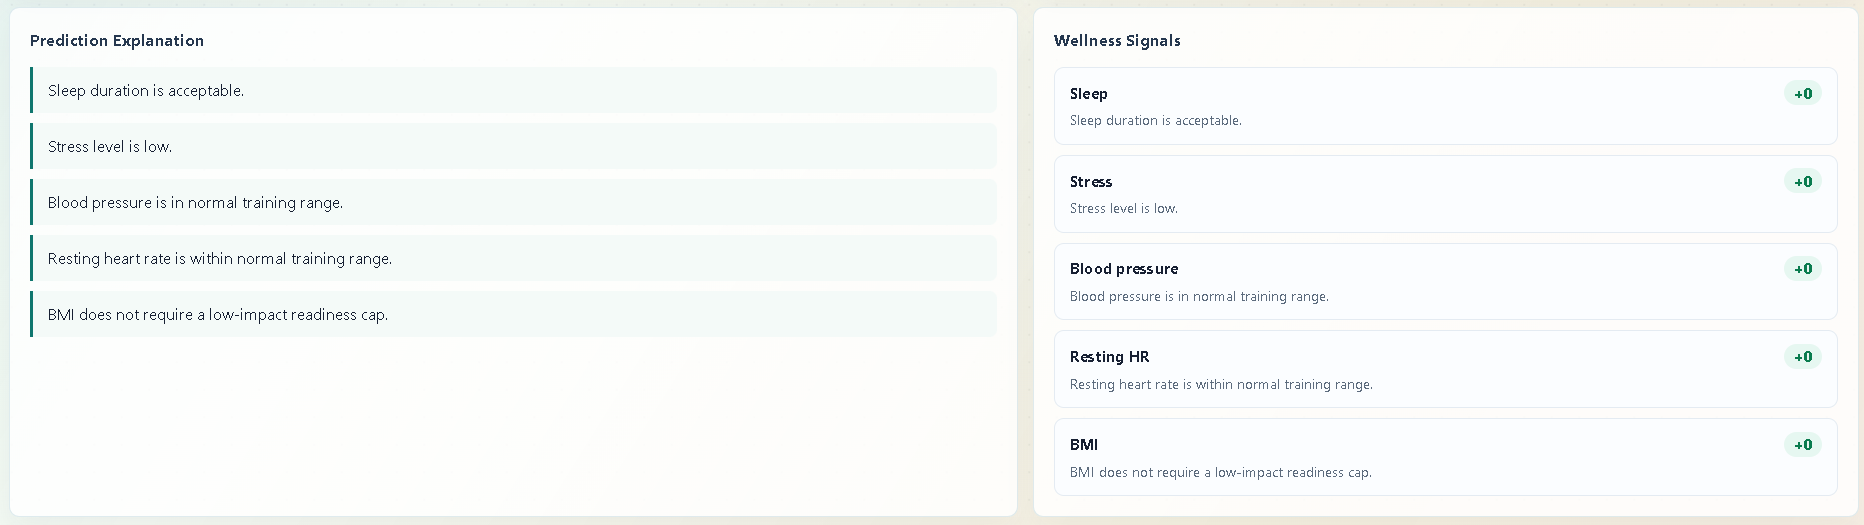
\includegraphics[width=\linewidth]{figures/Dashboard Figure/Client Profile and Readiness Inputs Before Result B.png}
        \caption{Result B}
    \end{subfigure}\\[3pt]
    \begin{subfigure}[t]{0.85\linewidth}
        \centering
        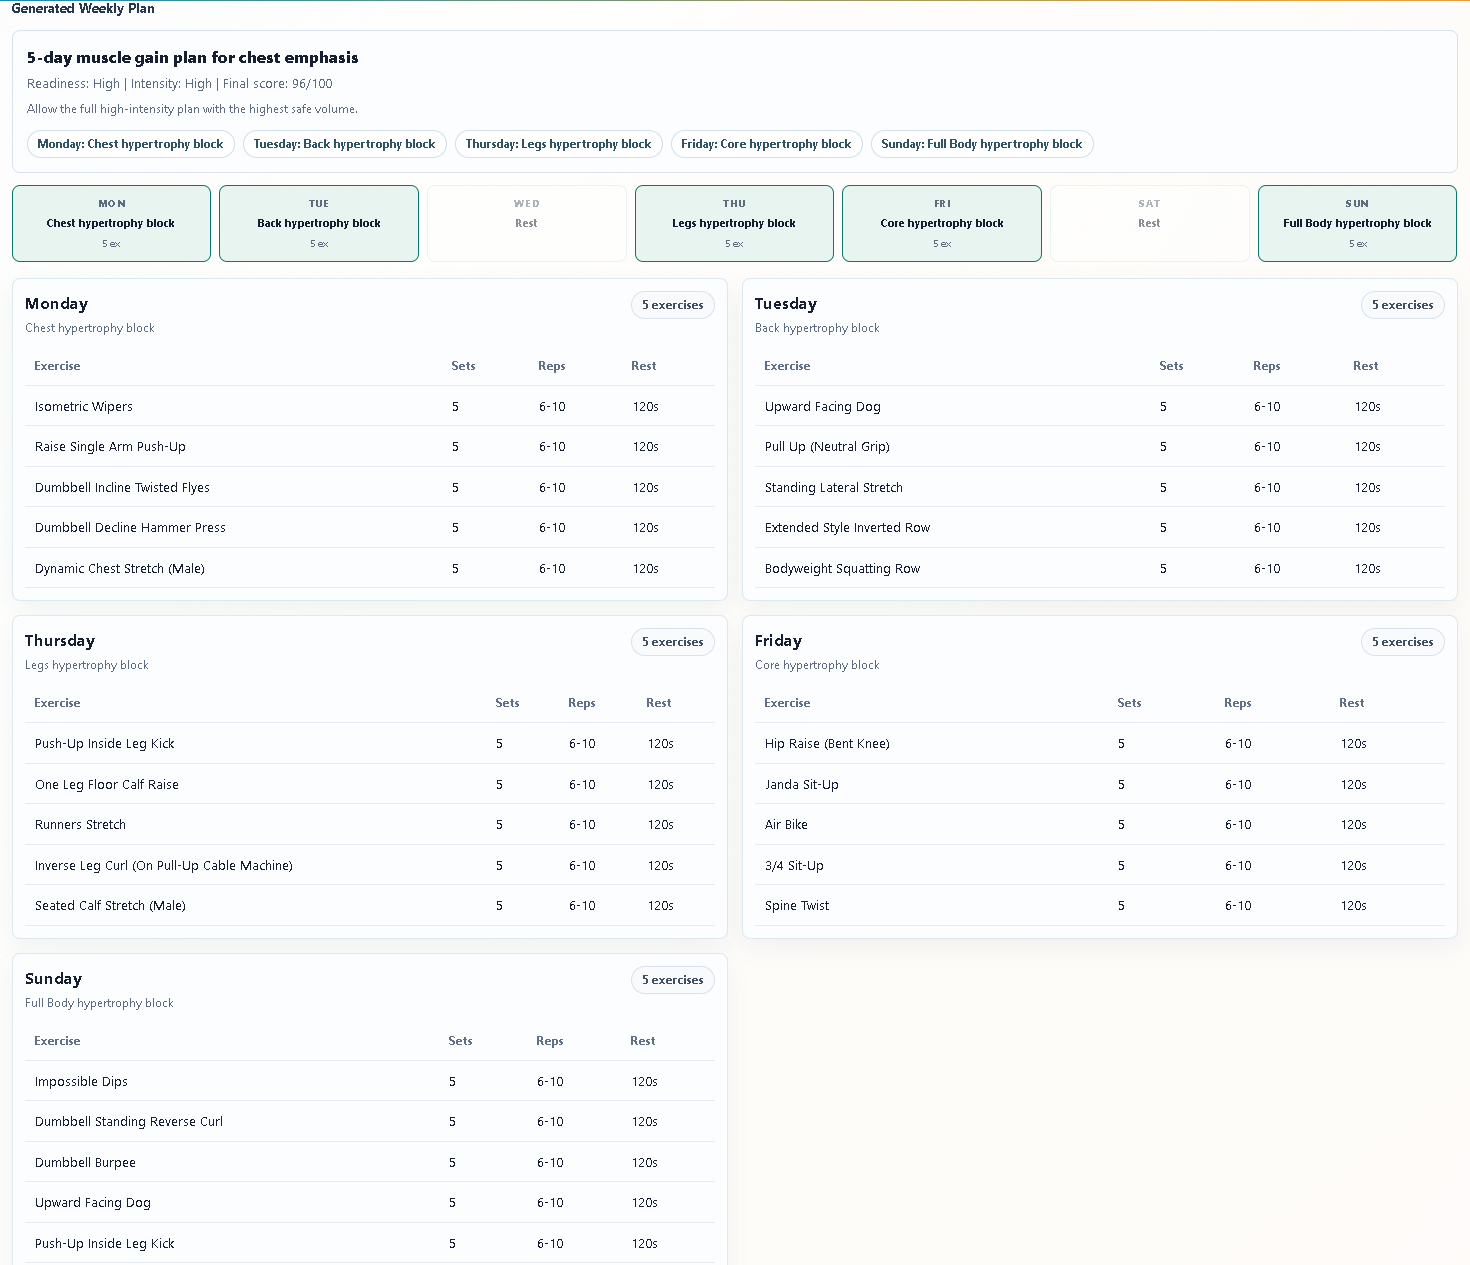
\includegraphics[width=\linewidth]{figures/Dashboard Figure/Client Profile and Readiness Inputs Before Result C.png}
        \caption{Result C}
    \end{subfigure}\\[3pt]
    \begin{subfigure}[t]{0.85\linewidth}
        \centering
        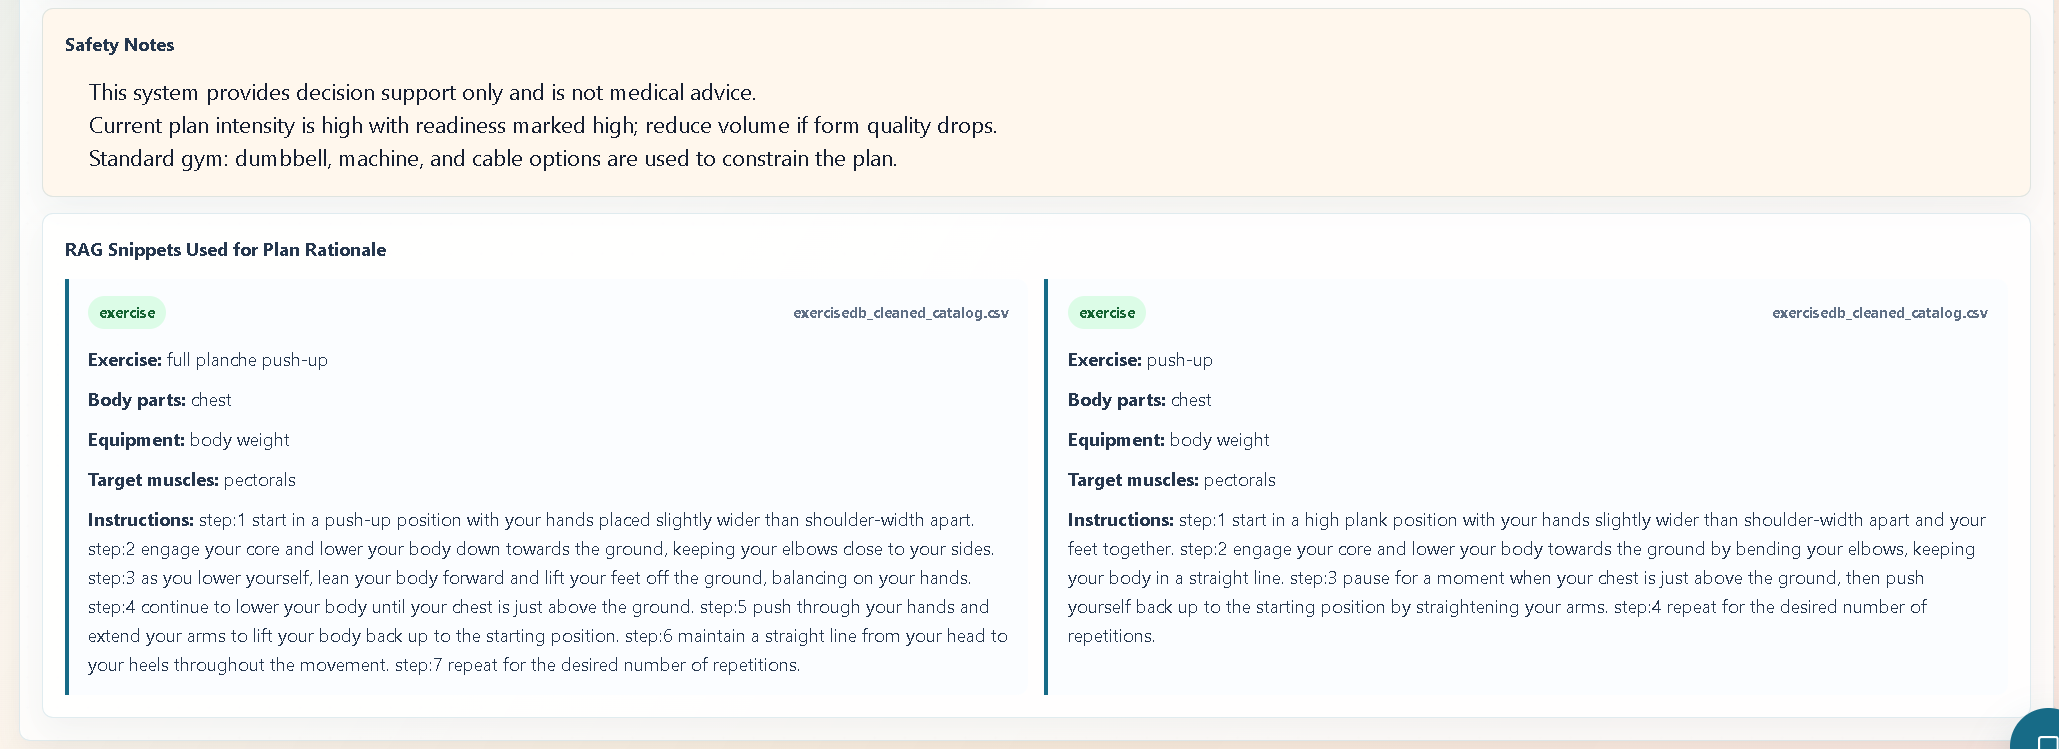
\includegraphics[width=\linewidth]{figures/Dashboard Figure/Client Profile and Readiness Inputs Before Result D.png}
        \caption{Result D}
    \end{subfigure}
    \caption{Additional readiness-result panels.}
    \label{fig:chapter4_client_profile_workflow_b}
\end{figure}

The additional readiness workflow figures show the full user path after form submission. The dashboard does not stop at a readiness score; it expands the result into plan guidance, adjustment advice, and context that the user can track during the week.
\begin{figure}[H]
    \centering
    \begin{subfigure}[t]{0.85\linewidth}
        \centering
        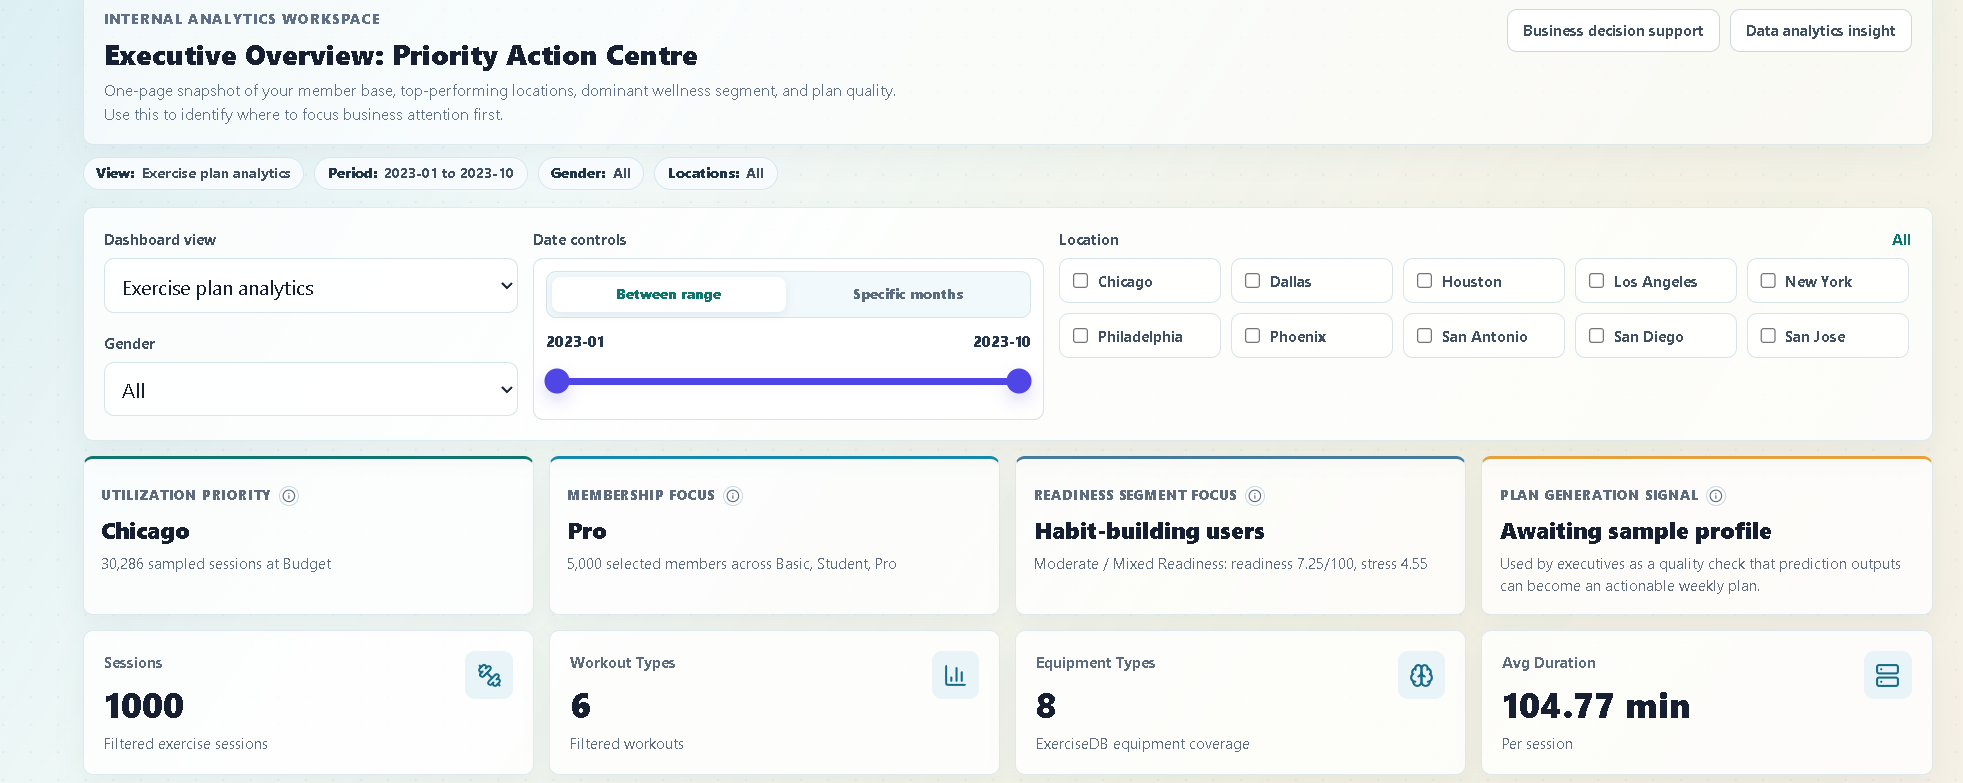
\includegraphics[width=\linewidth]{figures/Dashboard Figure/Exercise Plan Analytics A.png}
        \caption{Plan output A}
    \end{subfigure}\\[3pt]
    \begin{subfigure}[t]{0.85\linewidth}
        \centering
        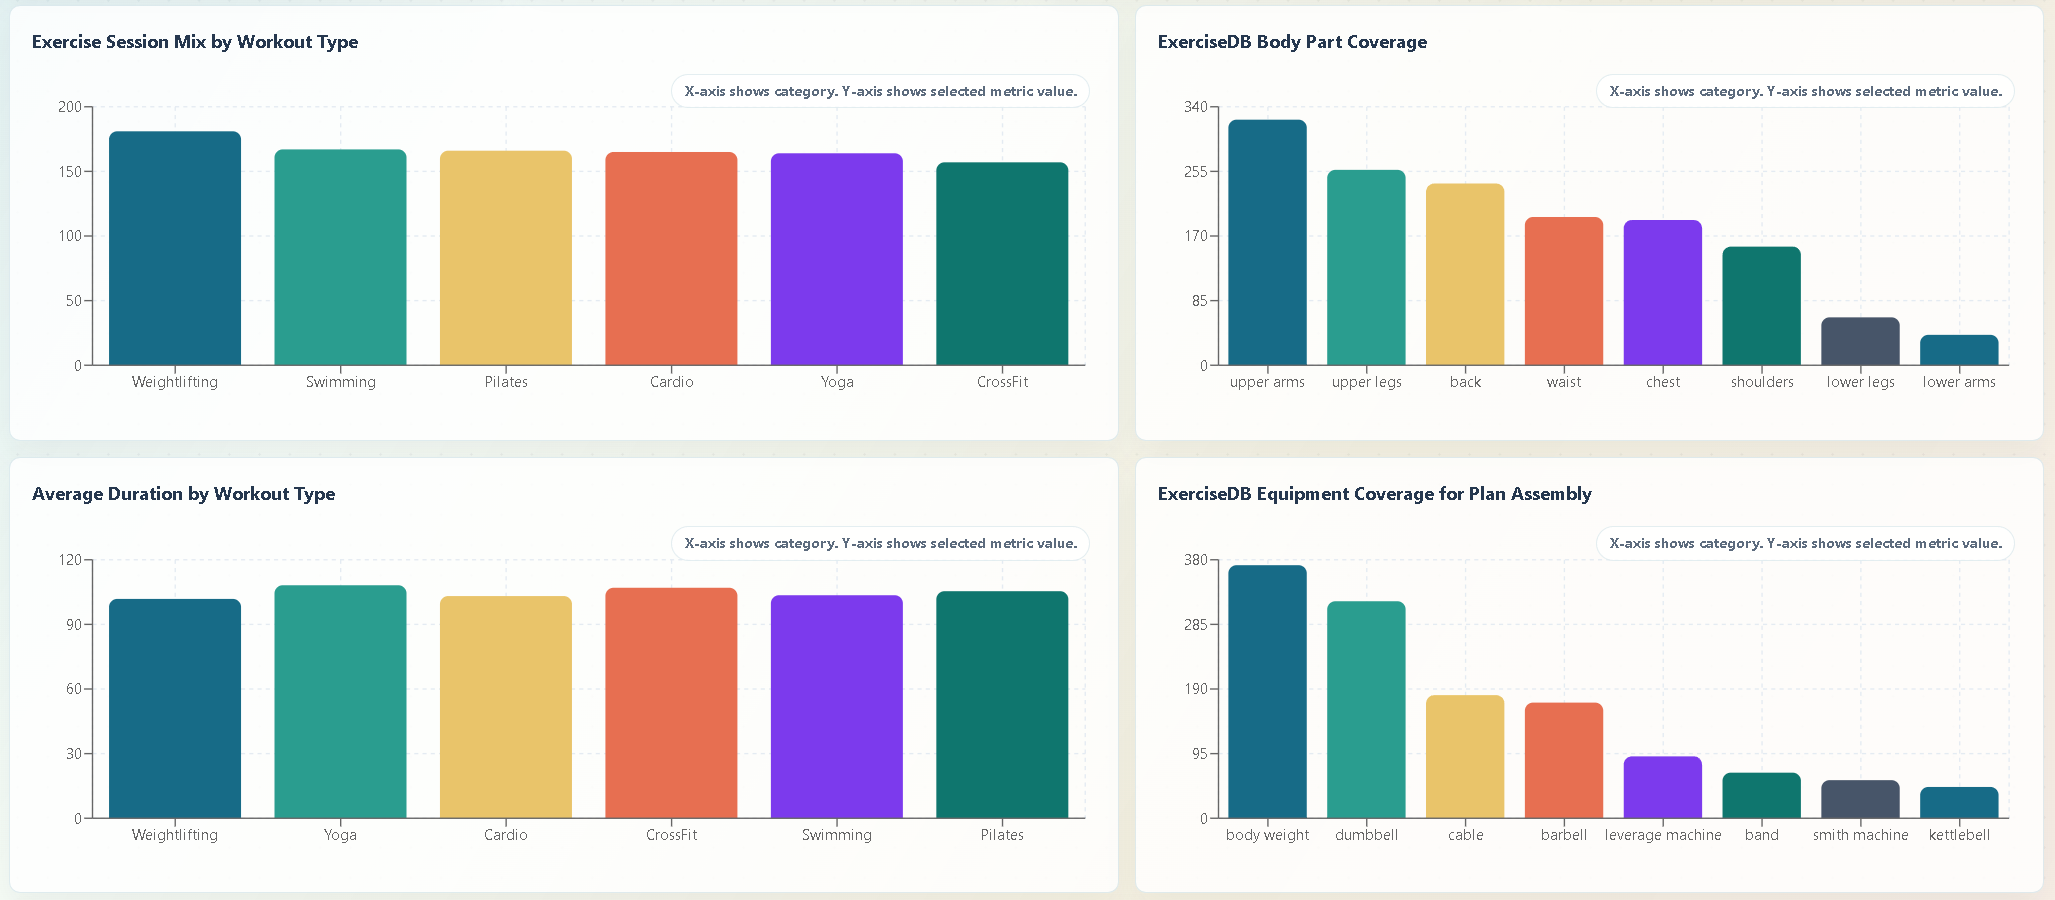
\includegraphics[width=\linewidth]{figures/Dashboard Figure/Exercise Plan Analytics B.png}
        \caption{Plan output B}
    \end{subfigure}\\[3pt]
    \begin{subfigure}[t]{0.85\linewidth}
        \centering
        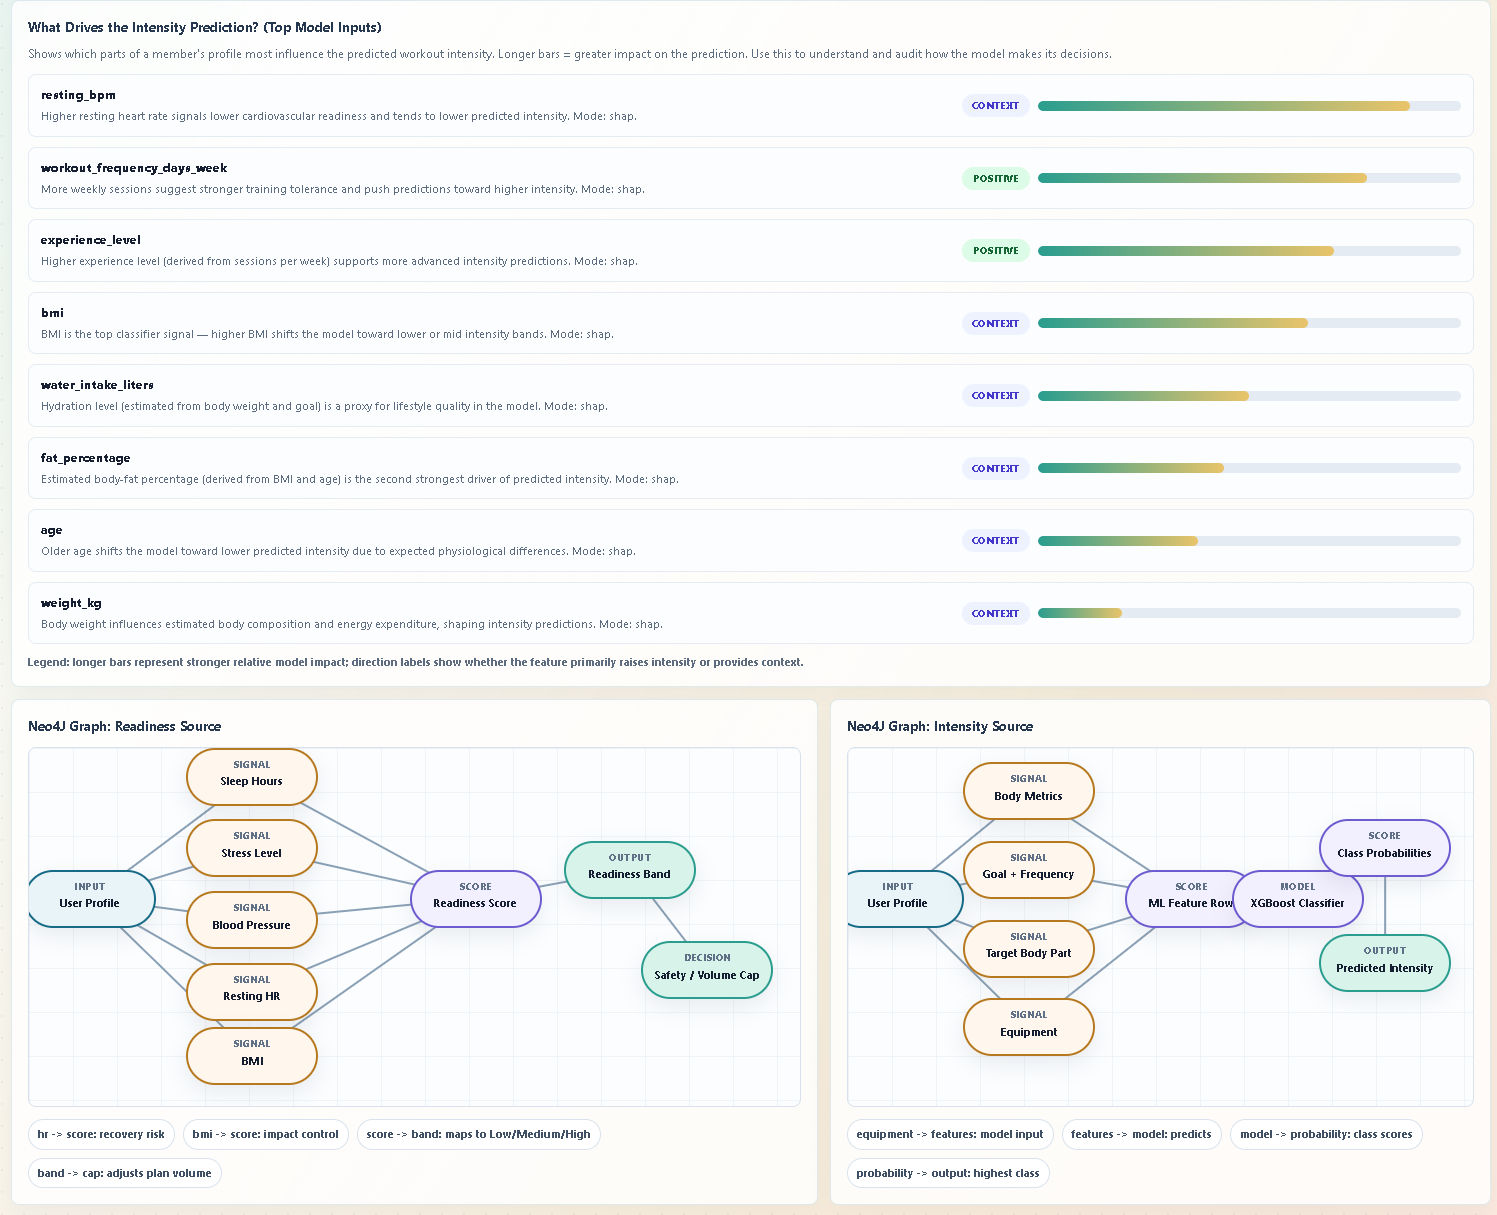
\includegraphics[width=\linewidth]{figures/Dashboard Figure/Exercise Plan Analytics C.png}
        \caption{Plan output C}
    \end{subfigure}
    \caption{Exercise plan analytics.}
    \label{fig:chapter4_exercise_plan}
\end{figure}

The exercise plan analytics result is the prescriptive output of the system. It connects the estimated calorie target and predicted intensity to concrete training terms such as exercise selection, weekly focus, and adjustment priority. This is the point where machine learning becomes an action plan rather than only a prediction.

This view also embeds two explainability panels that extend the model transparency goal from Chapter 2 into the live dashboard rather than leaving it as an offline diagnostic. A feature-impact panel renders the same SHAP values produced by \path{train_week2_ml.py} for the selected intensity classifier (Figure~\ref{fig:chapter4_exercise_plan}, panel C), so the classifier's top drivers are visible to the user at prediction time rather than only in the Appendix~B diagnostic plots. Alongside it, two static lineage diagrams trace how the readiness score and the predicted intensity class are each derived, step by step, from raw profile inputs through to the final band or class. These diagrams are illustrative node-and-edge visualizations rather than live queries against a graph database; they exist to make the rule-based and model-based decision paths auditable at a glance, complementing the numeric readiness and intensity results discussed above.

\begin{figure}[H]
    \centering
    \begin{subfigure}[t]{0.6\linewidth}
        \centering
        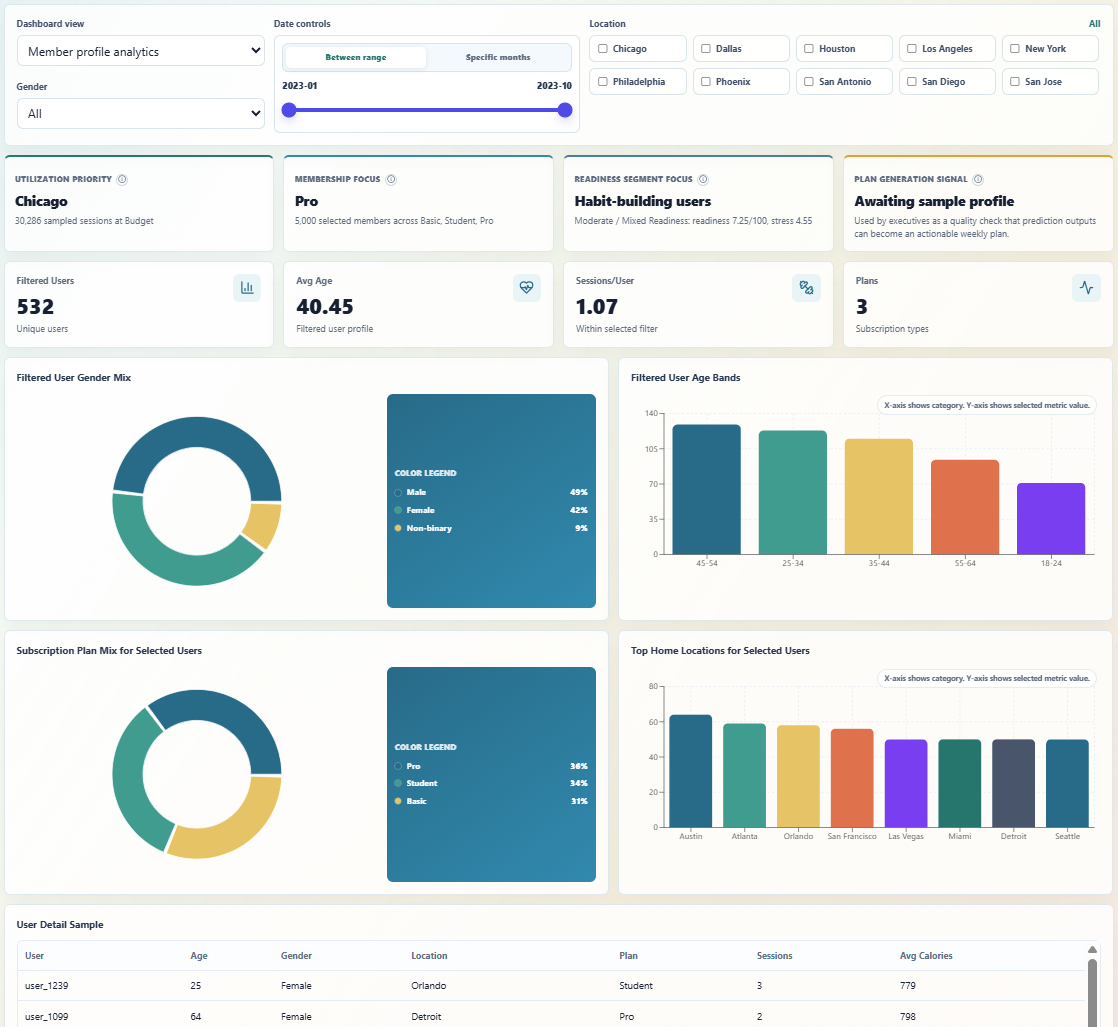
\includegraphics[width=\linewidth]{figures/Dashboard Figure/Member-Profile01.png}
        \caption{Member profile result}
    \end{subfigure}\\[3pt]
    \begin{subfigure}[t]{0.6\linewidth}
        \centering
        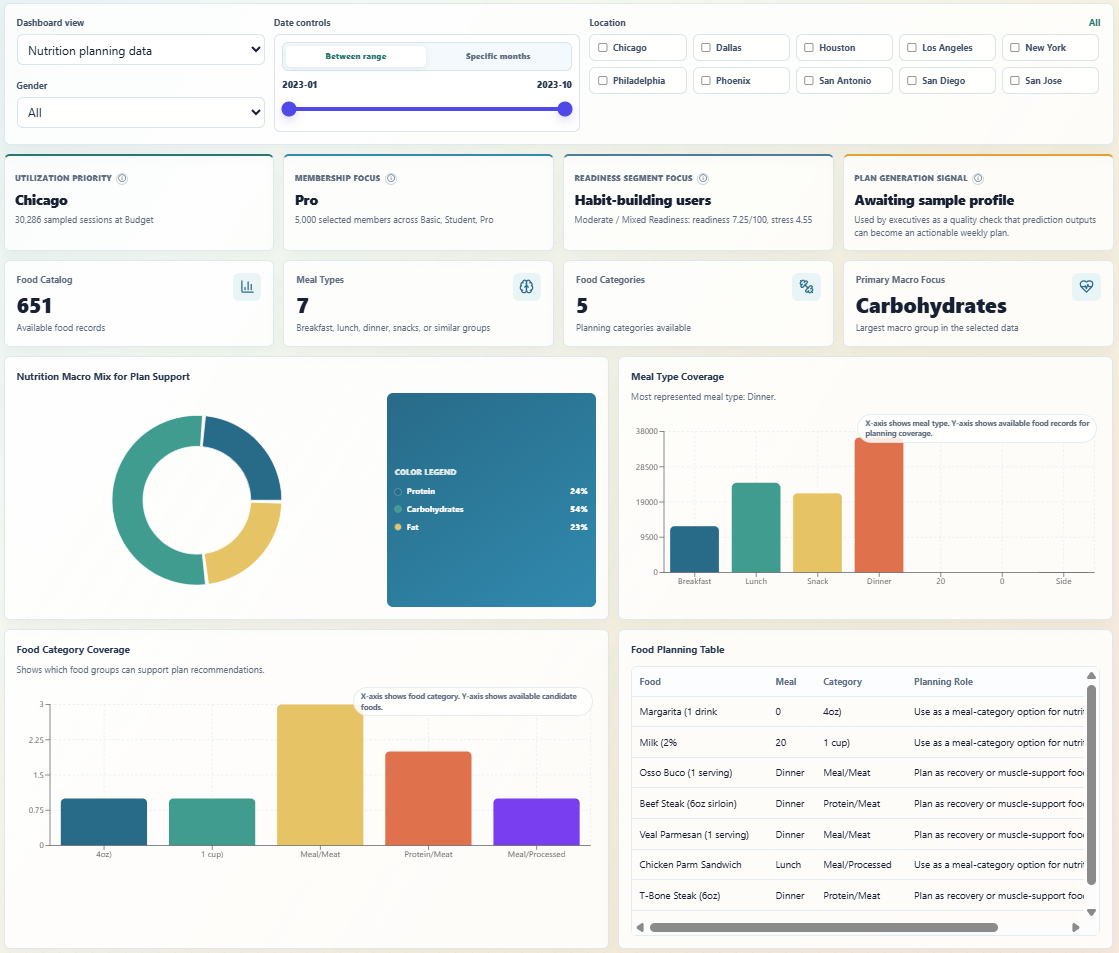
\includegraphics[width=\linewidth]{figures/Dashboard Figure/Nutrition01.png}
        \caption{Nutrition result}
    \end{subfigure}
    \caption{User profile and nutrition dashboard outputs.}
    \label{fig:chapter4_member_nutrition}
\end{figure}

The member profile and nutrition result completes the user loop. It gives the user a way to monitor weekly indicators that can improve readiness and consistency, including activity context, nutrition signals, and profile-related constraints.



\section{RAG}

The dashboard views above already surface RAG-grounded output -- the plan rationale and assistant chat panels shown later in this section are dashboard components -- so this closing section explains the retrieval mechanism that makes those panels trustworthy rather than merely generated text.

The RAG layer supports the user-facing plan output and chat explanation. It indexes exercise instructions, equipment options, target body parts, and plan-rationale snippets with ChromaDB and sentence embeddings. During inference, the system retrieves relevant exercise and rule context before presenting the workout plan. This reduces the chance that the recommendation becomes only a generic text response; the final plan is grounded in retrieved exercise evidence and constrained by the user's readiness, predicted intensity, equipment, and target muscle group.

\begin{table}[htbp]
\centering
\small
\caption{RAG input, retrieval, and output behavior.}
\label{tab:chapter4_rag_io}
\begin{tabularx}{\linewidth}{p{3.2cm}p{3.7cm}X}
\toprule
\textbf{Input} & \textbf{Retrieved evidence} & \textbf{Output result} \\
\midrule
User goal, target body part, equipment, and constraints & ExerciseDB instructions, equipment alternatives, and body-part matching rules & Personalized exercise list with sets, reps, and practical weekly training guidance. \\[10pt]
Readiness score, sleep, stress, activity level, and predicted intensity & Readiness rules and plan-adjustment snippets & Priority adjustment such as reducing intensity, increasing recovery, or maintaining progressive load. \\[10pt]
User chat question about a plan component & Relevant exercise instructions and substitution context & Natural-language explanation that links the recommendation to the user's profile and retrieved evidence. \\
\bottomrule
\end{tabularx}
\end{table}

The RAG result is most valuable for the user questions that ask why a plan was generated and what should be adjusted first. For example, when readiness is low, the system can explain whether the highest-priority action is sleep recovery, stress reduction, lower intensity, or a smaller weekly workload. This gives the user a practical reason for the plan output rather than only displaying a prediction score.

\begin{figure}[H]
    \centering
    \begin{subfigure}[t]{0.85\linewidth}
        \centering
        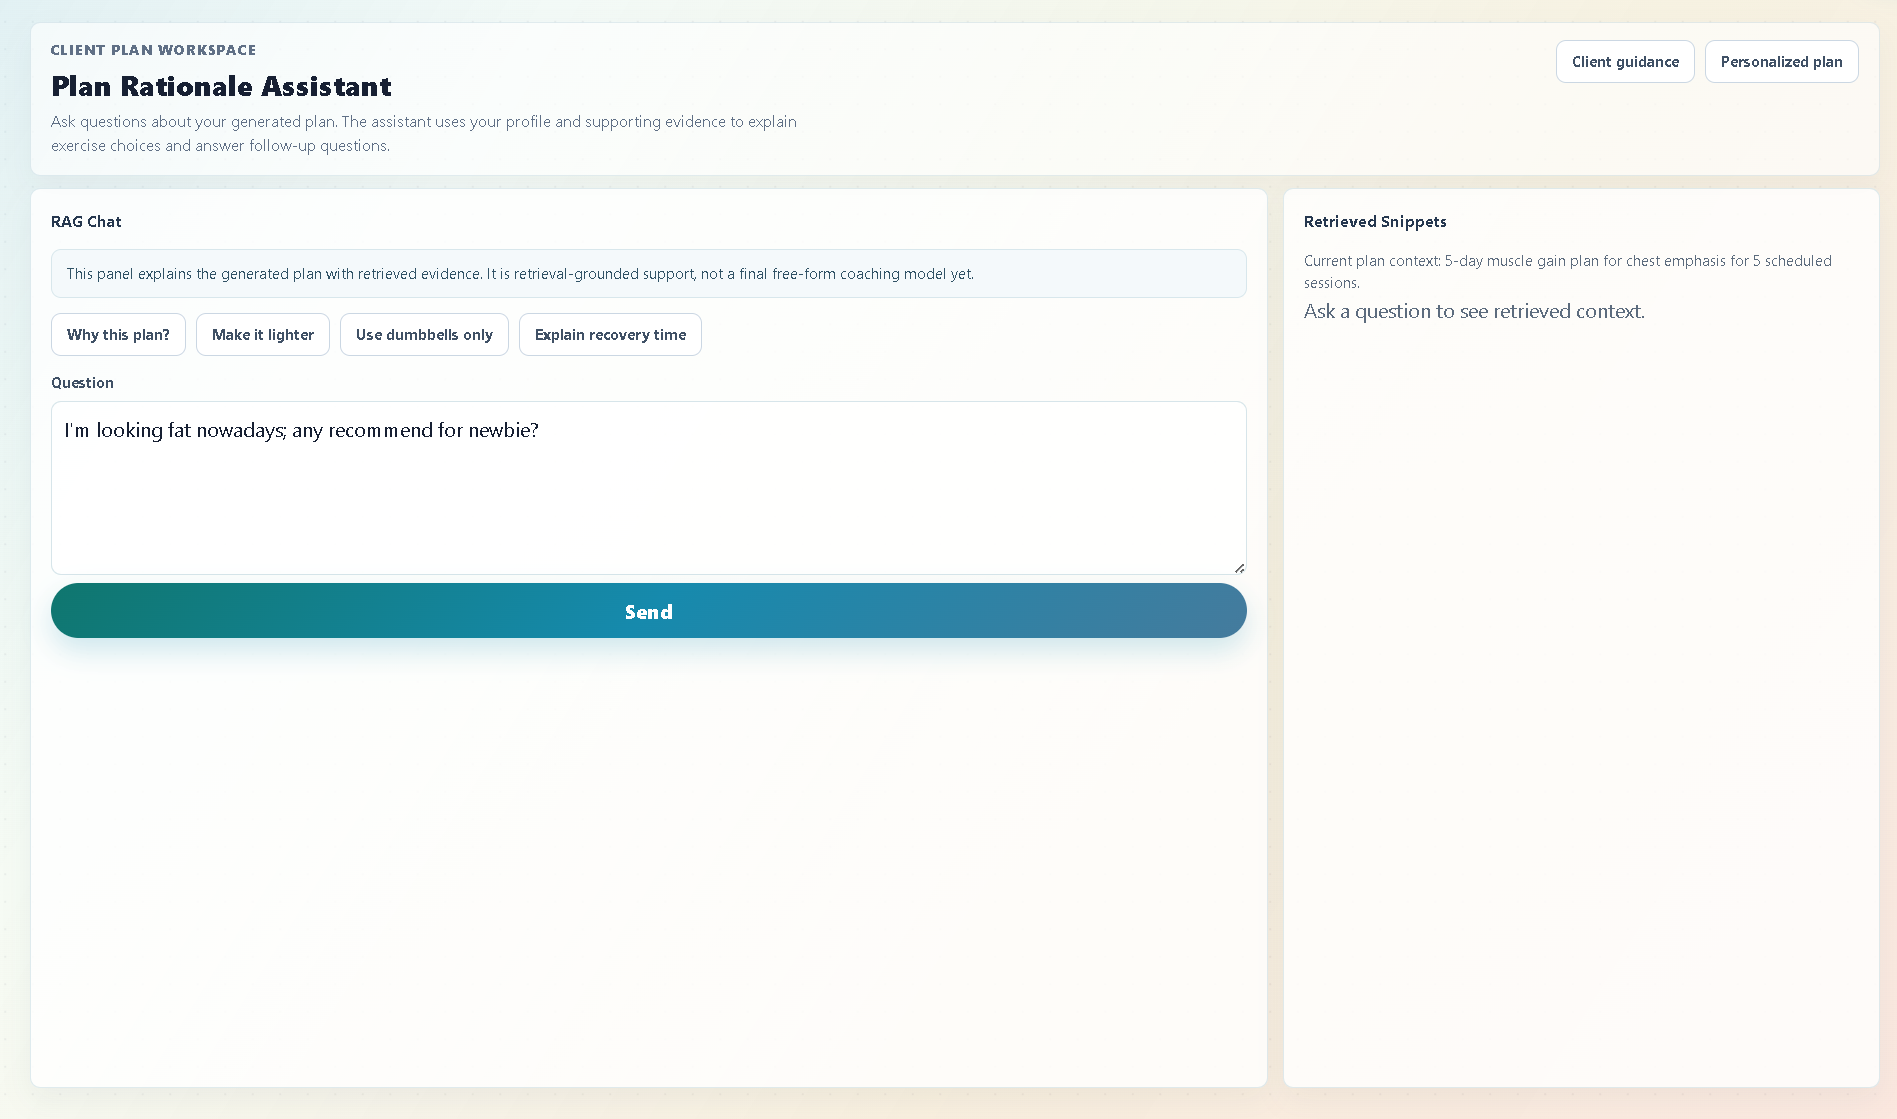
\includegraphics[width=\linewidth]{figures/Dashboard Figure/Plan Rational Assistant.png}
        \caption{Plan rationale assistant input}
    \end{subfigure}\\[3pt]
    \begin{subfigure}[t]{0.85\linewidth}
        \centering
        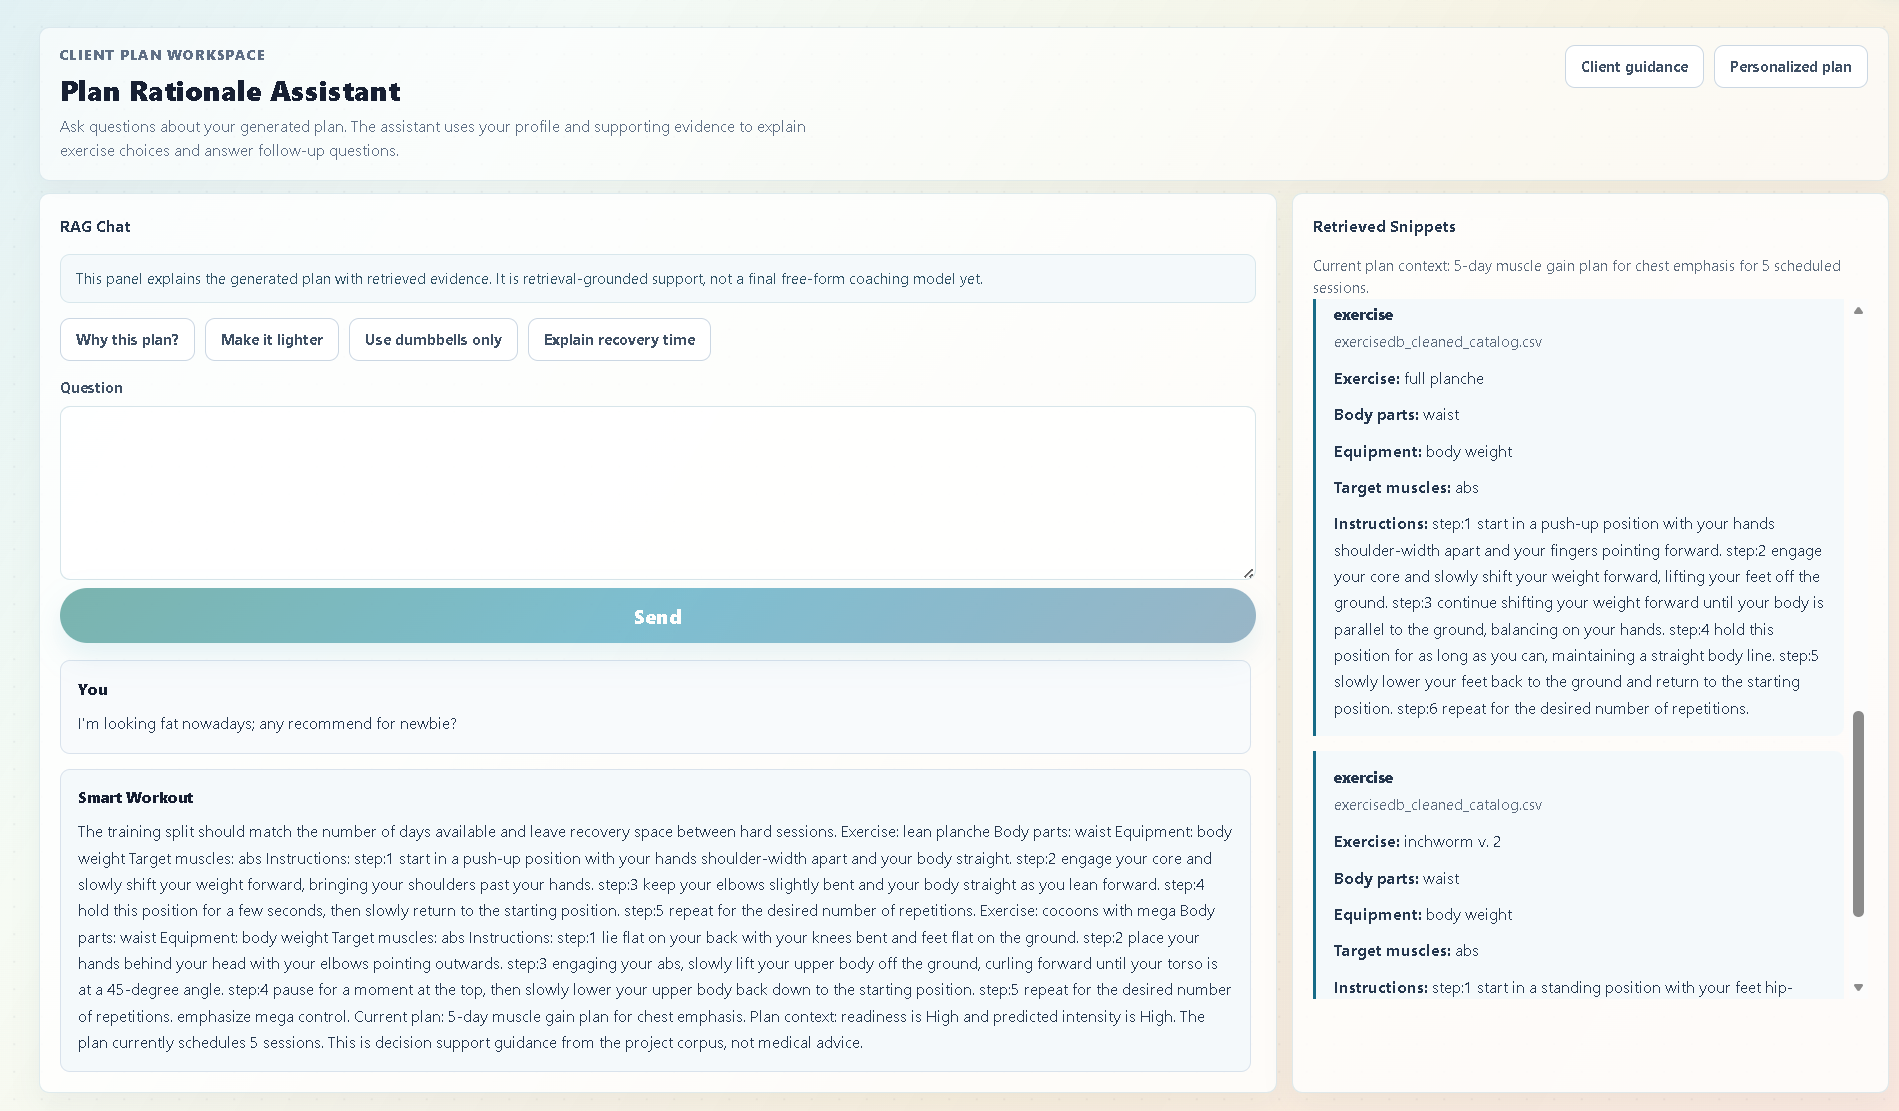
\includegraphics[width=\linewidth]{figures/Dashboard Figure/Plan Rational Assistant Result.png}
        \caption{Plan rationale assistant result}
    \end{subfigure}
    \caption{RAG-assisted plan rationale explaining a personalized recommendation.}
    \label{fig:chapter4_plan_rationale_assistant}
\end{figure}

\begin{figure}[H]
    \centering
    \begin{subfigure}[t]{0.47\linewidth}
        \centering
        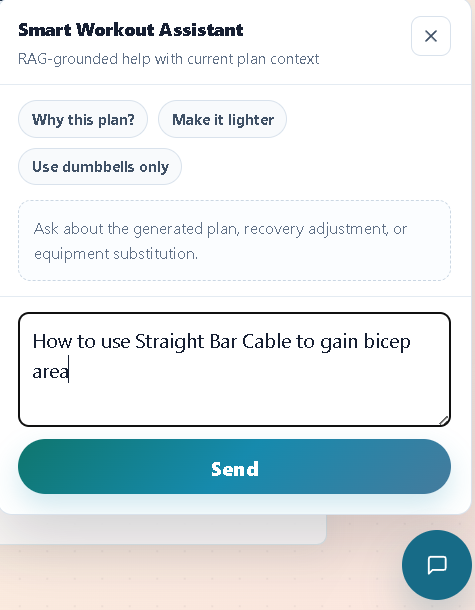
\includegraphics[width=\linewidth]{figures/Dashboard Figure/Smart Workout Assistant Chat.png}
        \caption{Assistant chat input}
    \end{subfigure}
    \hfill
    \begin{subfigure}[t]{0.47\linewidth}
        \centering
        
\includegraphics[width=\linewidth]{figures/Dashboard Figure/Smart Workout Assistant Chat Reply.png}
        \caption{Assistant chat reply}
    \end{subfigure}
    \caption{Assistant chat interface for plan and exercise questions.}
    \label{fig:chapter4_smart_workout_assistant}
\end{figure}

These RAG dashboard outputs show that the prescriptive layer is explainable at the interface level. The user can ask why the plan was produced, review the rationale, and receive a response that connects the retrieved exercise context to readiness, intensity, and weekly training constraints.

Overall, Chapter 4 shows that the project delivers more than isolated charts or models. The dataset evidence identifies operational patterns, the model-selection results provide transparent predictive evidence, the dashboard turns these outputs into business and user decisions, and the RAG layer closes the chapter by grounding those prescriptive plans and explanations in retrieved evidence rather than unconstrained generation.
% ==================== CHAPTER 5 ====================
\chapter{CONCLUSION AND RECOMMENDATIONS}
\section{Conclusion}

This project developed Smart Workout as an integrated Decision Support System and Business Intelligence dashboard for personalized weight training. The final system combines feature engineering, descriptive analytics, predictive machine learning, RAG-grounded exercise retrieval, and rule-based plan generation into one workflow. The main contribution is that the system does not stop at reporting data or predicting a label; it converts raw records into decision-ready signals, turns model outputs into plan guidance, and presents those outputs through dashboard views designed for both executive and individual users.

The dataset and feature-engineering results show that the project successfully transformed multiple independent data sources into usable analytical features. Gym membership and check-in records were converted into utilization, time-pattern, subscription, and estimated revenue signals. Exercise tracking and user-profile data were converted into calorie-burn-rate and intensity features. Lifestyle, sleep, stress, and activity inputs were converted into readiness scores and readiness bands. These engineered results enabled the dashboard to connect branch-level business questions with user-level training decisions.

The predictive layer produced transparent, deployment-aware model results. The XGBoost Regressor was selected for calorie-burn-rate estimation with RMSE 15.021 kcal/hr and $R^2=0.970$; this figure is reported as an upper bound rather than an expected deployment score, because its dominant feature, average BPM, is estimated from predicted intensity at inference rather than measured directly. For intensity classification, the XGBoost Classifier was selected on macro-F1 because the Low, Mid, and High classes are imbalanced. Reported honestly, the model beats majority-class and stratified-random baselines on macro-F1 but falls below the majority baseline on raw accuracy, and minority-class recall remains weak, especially for Low intensity at 21.5\% and High intensity at 29.3\%. Label leakage was prevented, gender was removed to avoid train/inference mismatch, and balanced weighting improved minority-class behavior. The classification task is therefore characterized as only partially successful in its current form, which is more useful for deployment decisions than an inflated headline number would be.

The RAG and dashboard results demonstrate that the system can translate predictions into explainable action. The RAG layer retrieves exercise instructions and substitution context to support plan rationale and assistant responses. The dashboard then presents executive summaries, membership utilization and revenue signals, lifestyle segments, readiness inputs, plan analytics, user profile context, nutrition context, and Tableau map integration. Together, these outputs answer the business decision questions about branch demand, cohort risk, segment readiness, weekday/weekend patterns, and prediction-to-plan consistency, while also helping individual users understand their readiness, predicted intensity, calorie target, and weekly action priority.

\section{Recommendations}

For executive users, Smart Workout should be used as a decision-support tool for monitoring branch utilization, segment demand, subscription-cohort behavior, and estimated revenue share. Managers should use the executive summary, membership utilization and revenue signals, lifestyle segment views, and Tableau map together rather than interpreting one chart in isolation. This combined view is most useful for identifying where staffing, campaign timing, capacity balancing, retention action, or upsell planning should be prioritized.

For individual users, the predicted intensity and calorie target should be interpreted as planning guidance rather than medical instruction. Users should review the readiness score, readiness band, primary action, plan rationale, and safety notes before following the generated weekly plan. When readiness is low, the highest priority should be recovery and controlled training volume. When readiness and predicted intensity are both high, the plan can support more progressive workload, but users should still monitor consistency, sleep, stress, and form quality.

For future dashboard use, the business mapping table in Chapter 4 should be treated as the operational guide. Each dashboard visual should be connected to a decision: utilization views support staffing and capacity choices, lifestyle segments support intervention prioritization, membership and revenue signals support retention or upsell actions, and user-plan analytics support weekly training adjustment. This keeps the dashboard from becoming only a set of charts and preserves its role as a decision-support system.

\section{Scope Limitations and Future Research Directions}

The current project is a prototype built from available academic and public datasets plus processed gym database records. It supports utilization analysis, subscription and cohort monitoring, estimated revenue signals, readiness scoring, workout-intensity prediction, calorie-burn-rate estimation, RAG-assisted exercise retrieval, and personalized plan generation. However, it does not directly observe true churn, profit, staffing rosters, equipment capacity, injury outcomes, long-term adherence, or verified member satisfaction. Therefore, retention risk, staffing overload, upsell potential, and readiness intervention priorities should be understood as decision-support proxies rather than confirmed business outcomes.

The predictive layer also has limitations. The regression result carries a specific caveat that qualifies its headline accuracy. Feature-attribution analysis in Figure~\ref{fig:appendix_calorie_shap} shows that average BPM is the most influential input to the calorie-burn-rate regressor. However, average BPM is not collected by the deployment form and is not measured during real use; at inference it is estimated from the predicted intensity class, which is itself a model output. The regressor's strongest signal is therefore partially circular under deployment conditions. This means the cross-validated $R^2=0.970$, obtained while average BPM was available as a clean training feature, likely overstates the accuracy achievable in true deployment. The honest deployment figure is unknown until the regressor is retrained and re-evaluated under one of two protocols: excluding average BPM entirely, or replacing average BPM during both training and evaluation with the same estimate produced by the deployment pipeline. Average BPM is the most consequential case because it is also the top SHAP feature, but it is not unique: Table~\ref{tab:feature_provenance} shows that roughly half of the regression feature set is rule-estimated rather than measured at inference, so the same retrain-and-re-evaluate discipline should eventually be applied to the full feature set, not only to average BPM.

The classifier is also intentionally evaluated under leakage-prevention constraints, which makes the task harder and keeps accuracy modest. The RAG layer is currently validated through retrieval behavior and example responses rather than formal precision-at-k or recall-at-k metrics, so future evaluation should add quantitative retrieval tests. Future work should collect deployment-form data, real workout outcomes, wearable-device signals, and longitudinal adherence labels so that the model can be retrained on inputs that match real usage more closely.

Future research should extend the system in five directions. First, the dashboard should connect to live operational data so that utilization, revenue, and cohort signals update automatically. Second, true churn, upgrade, satisfaction, and retention labels should be added to validate the business decision questions. Third, the RAG layer should be expanded with coach-reviewed training rules, injury constraints, and nutrition guidance. Fourth, user feedback after following a plan should be collected to improve readiness scoring and plan personalization. Finally, the Tableau integration can be expanded from a single location map into a multi-view embedded workbook covering revenue share, cohort retention, and utilization forecasting.

Overall, Smart Workout demonstrates that a BI dashboard, machine learning layer, RAG knowledge layer, and rule-based workout planner can be combined into one explainable decision-support prototype. The strongest outcome of the project is the connection between data engineering, transparent predictive evaluation, grounded recommendations, and dashboard-based action decisions.
% ==================== REFERENCES ====================

\cleardoublepage
\phantomsection
\addcontentsline{toc}{chapter}{\bf REFERENCES}
\nocite{amoghabhinavms2024,exercisedb,khorasani2024,shamim2025,tharmalingam2023}
\renewcommand{\bibname}{REFERENCES}
\bibliographystyle{apacite}
\bibliography{references}

% ==================== APPENDIX ====================

\clearpage
\phantomsection
\addcontentsline{toc}{chapter}{\bf APPENDICES}
\begin{center}
    \vspace*{\fill}
    \large{\bf APPENDICES}
    \vspace*{\fill}
\end{center}
\clearpage

\appendix
\renewcommand{\appendixname}{APPENDIX}
\renewcommand\thefigure{\thechapter\arabic{figure}}
\renewcommand\thetable{\thechapter\arabic{table}}
\captionsetup[table]{labelfont=bf,name=Table\space,labelsep=space}
\captionsetup[figure]{labelfont=bf,name=Figure\space,labelsep=space}

\chapter{SOURCE CODE AVAILABILITY}

The complete source code for Smart Workout is available at:

\begin{center}
\texttt{https://github.com/Smart-Workout/125970-125934-125843-BIA.git}
\end{center}

A live deployment is accessible at: 

\begin{center}
\url{https://smart-workout-frk3.onrender.com}
\end{center}

The repository includes:
\begin{itemize}
    \item Source code
    \item Backend API
    \item Frontend
    \item Documentation
\end{itemize}

\clearpage

\chapter{EXPLORATORY DATA ANALYSIS FIGURES}

The following appendix figures provide the detailed EDA and model-diagnostic evidence used during dashboard design. They are placed in the appendix to keep Chapter 4 focused on dashboard results and decision interpretation while still documenting the observed data patterns behind the analysis.

\begin{figure}[H]
    \centering
    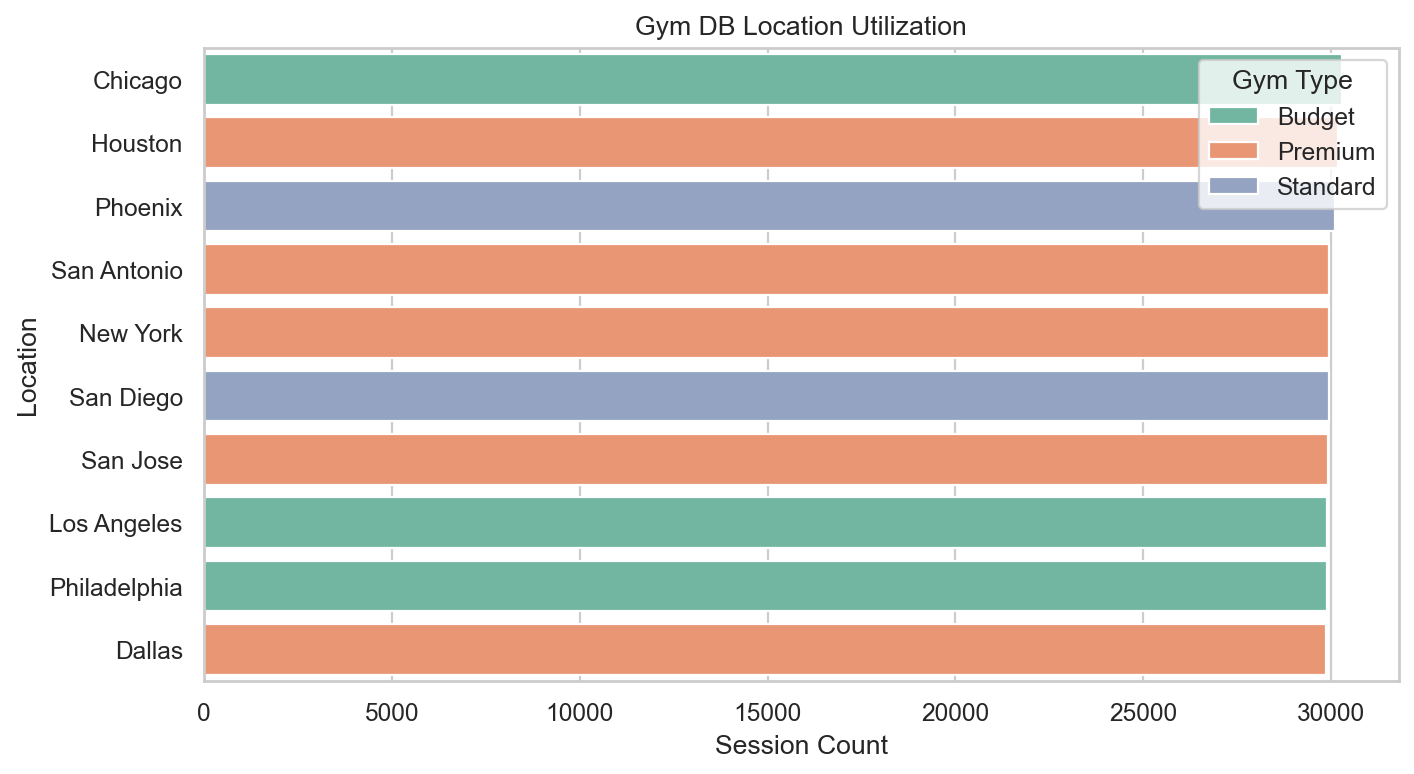
\includegraphics[width=0.86\linewidth]{../docs/figures/week1/gymdb_location_utilization.png}
    \caption{EDA: Gym DB location utilization.}
\end{figure}

\begin{figure}[H]
    \centering
    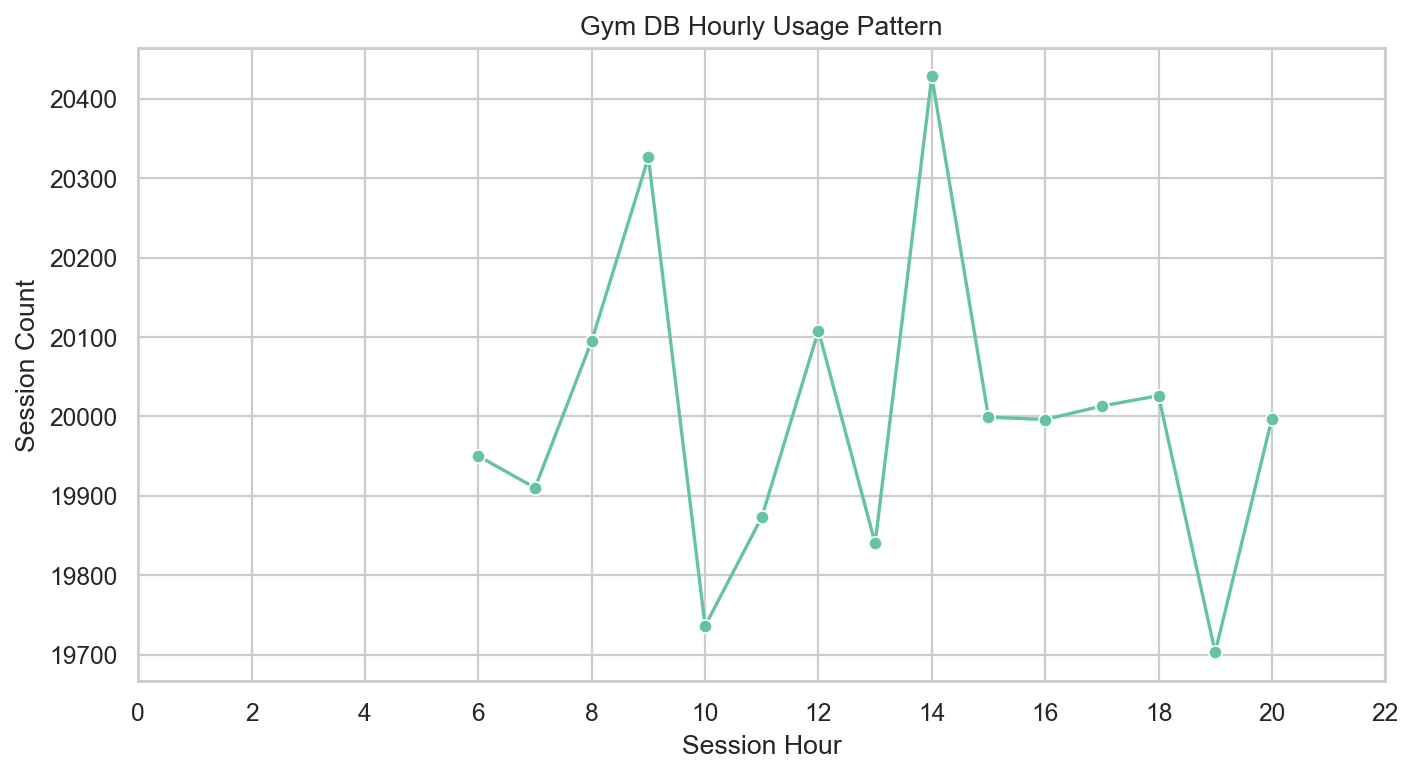
\includegraphics[width=0.86\linewidth]{../docs/figures/week1/gymdb_hourly_usage_pattern.png}
    \caption{EDA: hourly gym usage pattern.}
\end{figure}

\begin{figure}[H]
    \centering
    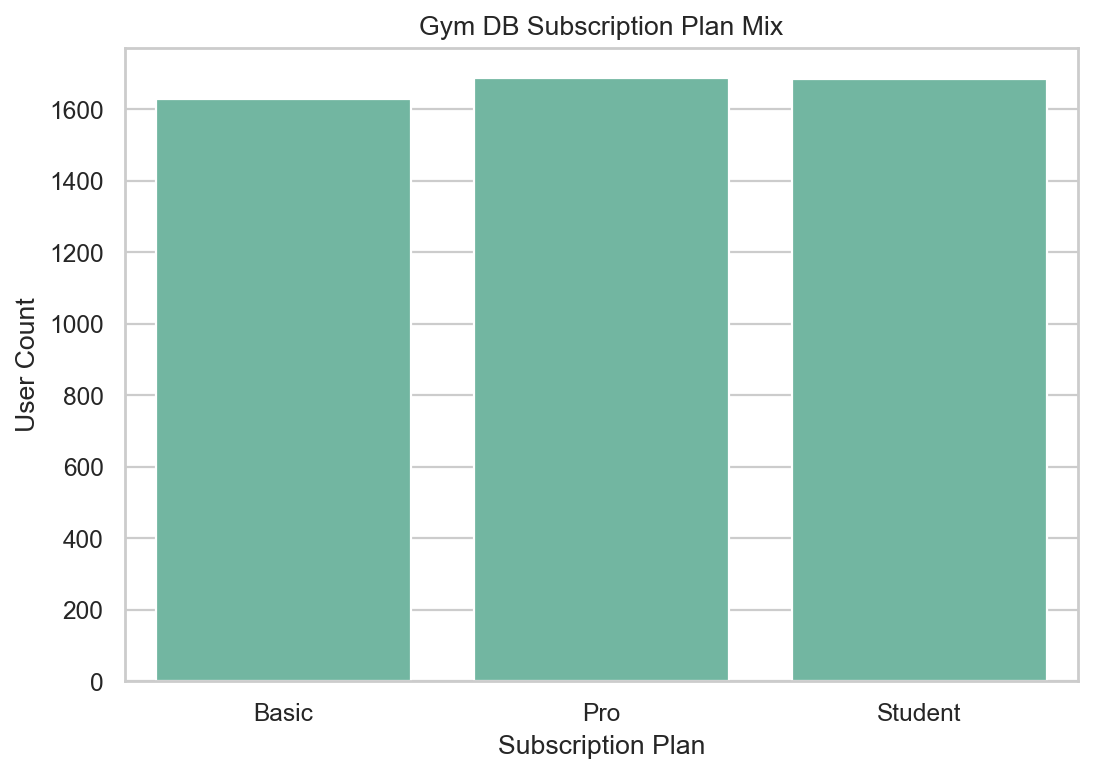
\includegraphics[width=0.86\linewidth]{../docs/figures/week1/gymdb_subscription_plan_mix.png}
    \caption{EDA: subscription plan mix.}
\end{figure}

\begin{figure}[H]
    \centering
    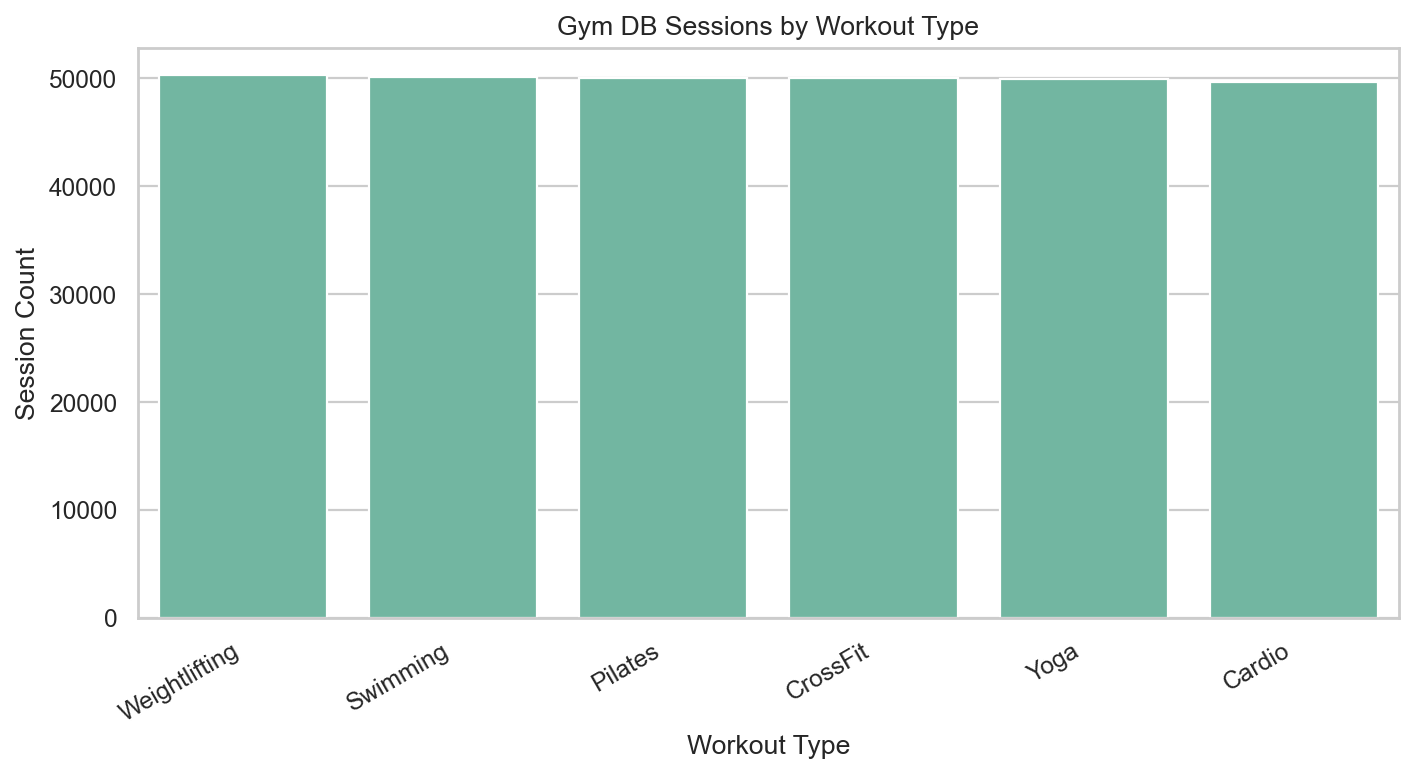
\includegraphics[width=0.86\linewidth]{../docs/figures/week1/gymdb_sessions_by_workout_type.png}
    \caption{EDA: Gym DB sessions by workout type.}
\end{figure}

\begin{figure}[H]
    \centering
    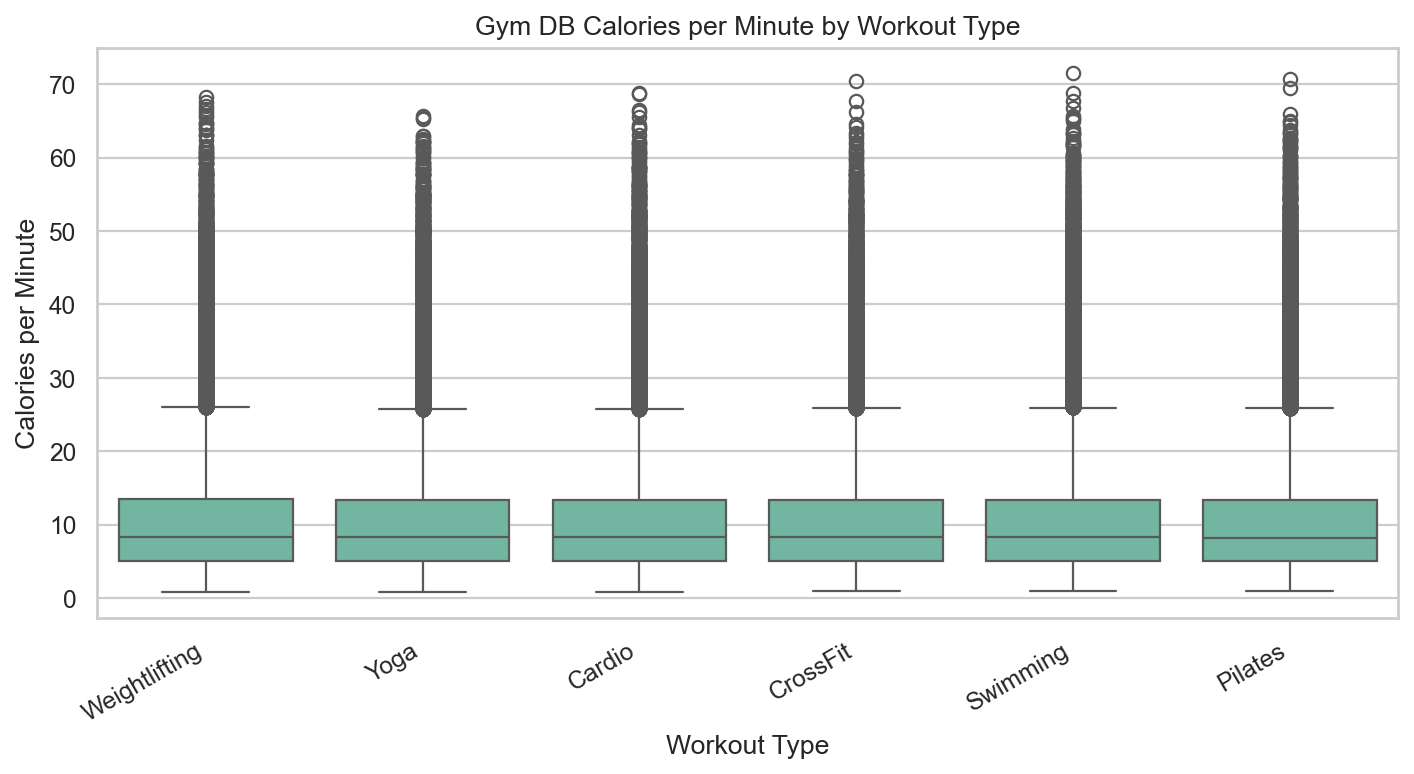
\includegraphics[width=0.86\linewidth]{../docs/figures/week1/gymdb_calories_per_minute_by_workout.png}
    \caption{EDA: calories per minute by workout type.}
\end{figure}

\begin{figure}[H]
    \centering
    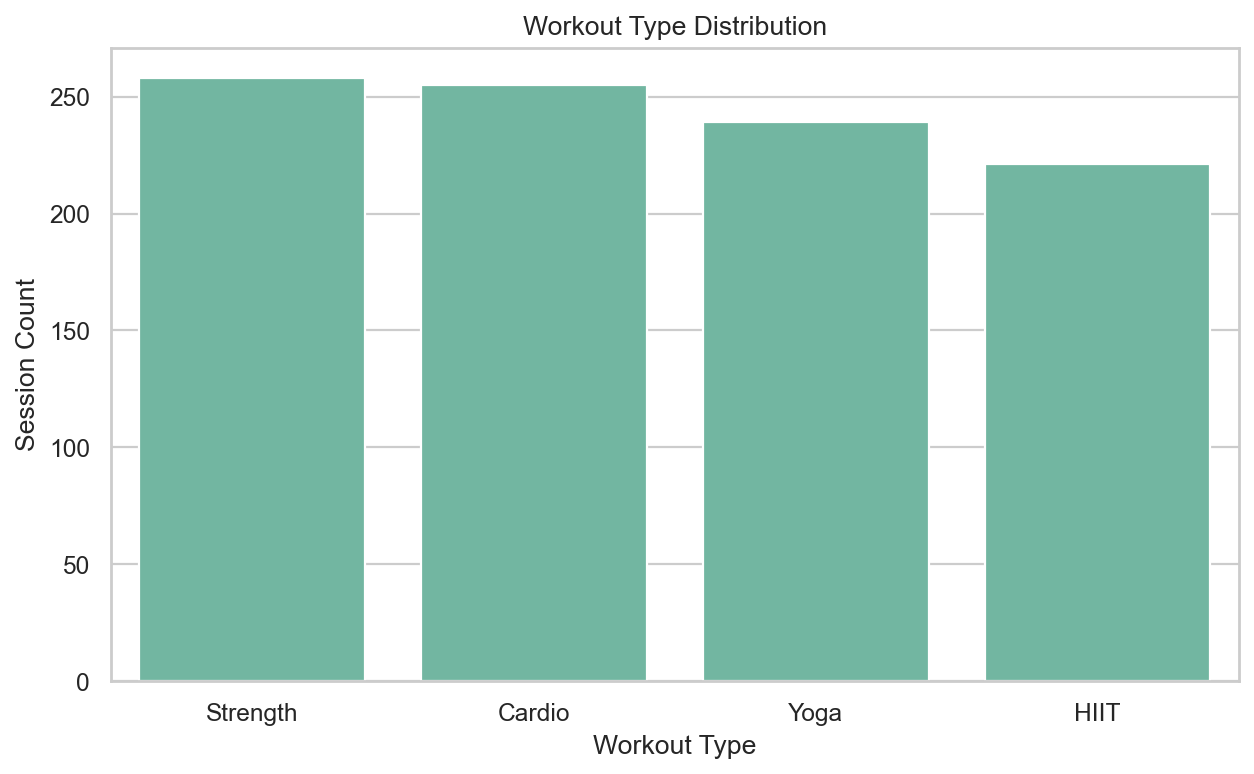
\includegraphics[width=0.86\linewidth]{../docs/figures/week1/workout_type_distribution.png}
    \caption{EDA: workout type distribution from exercise tracking data.}
\end{figure}

\begin{figure}[H]
    \centering
    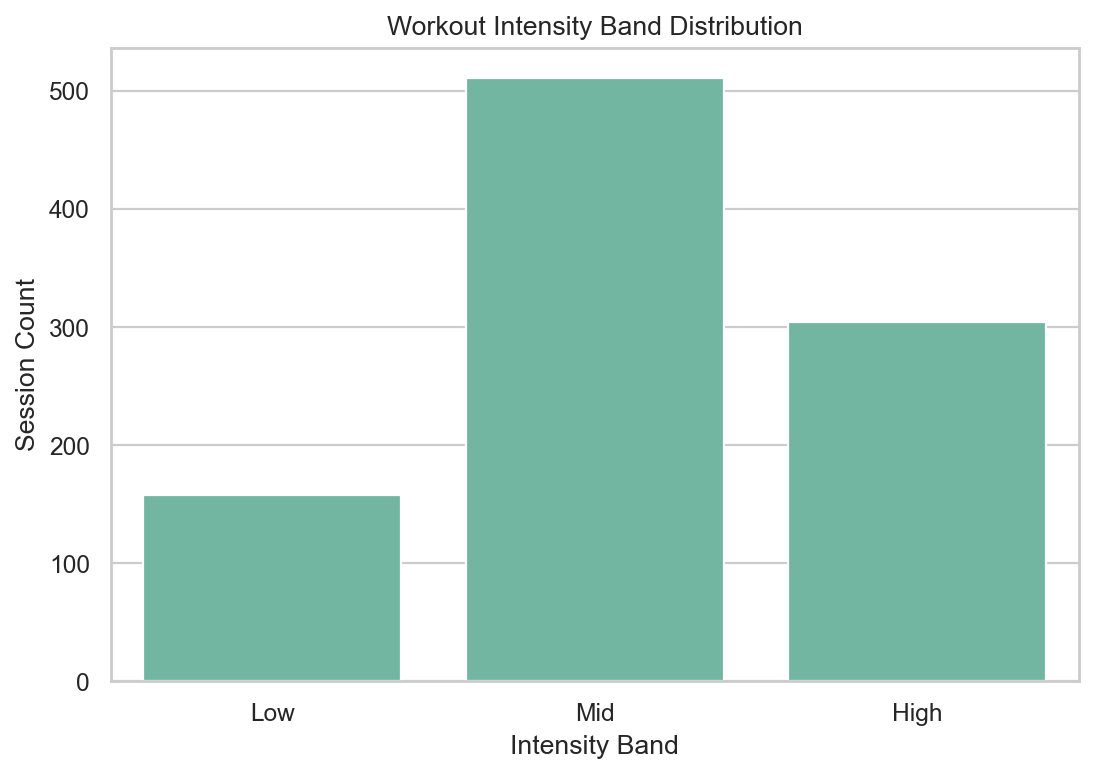
\includegraphics[width=0.86\linewidth]{../docs/figures/week1/intensity_band_distribution.png}
    \caption{EDA: workout-intensity band distribution.}
\end{figure}

\begin{figure}[H]
    \centering
    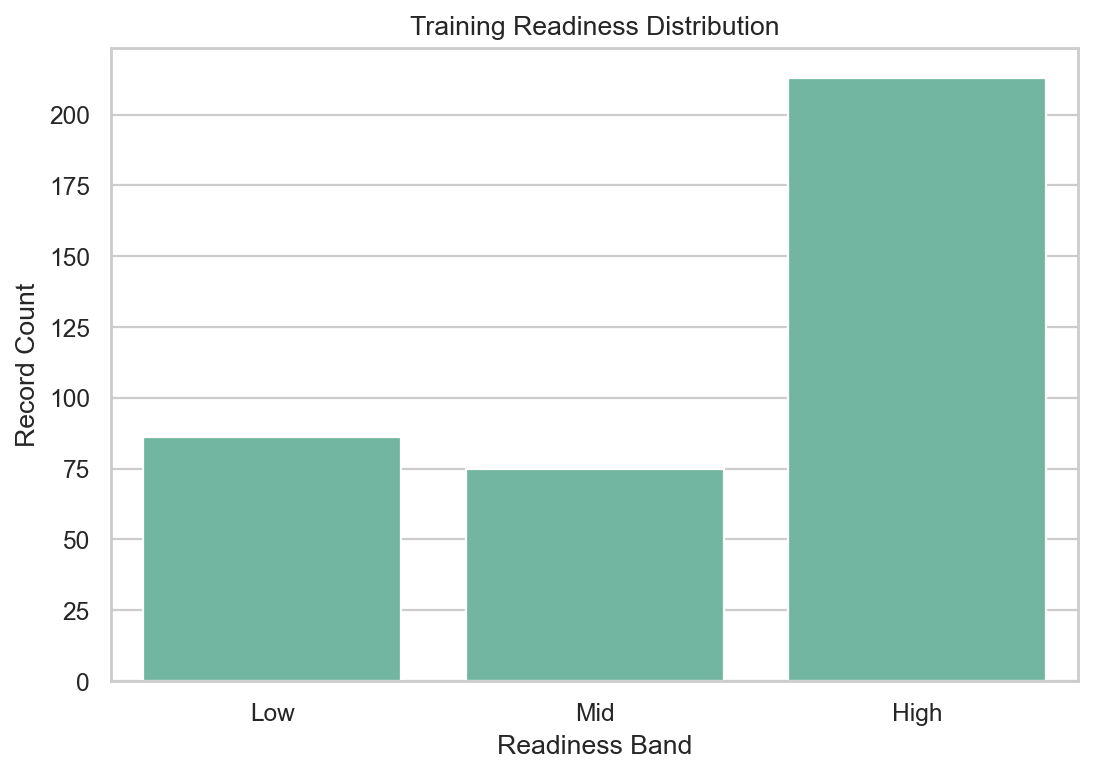
\includegraphics[width=0.86\linewidth]{../docs/figures/week1/training_readiness_distribution.png}
    \caption{EDA: training readiness distribution.}
\end{figure}

\begin{figure}[H]
    \centering
    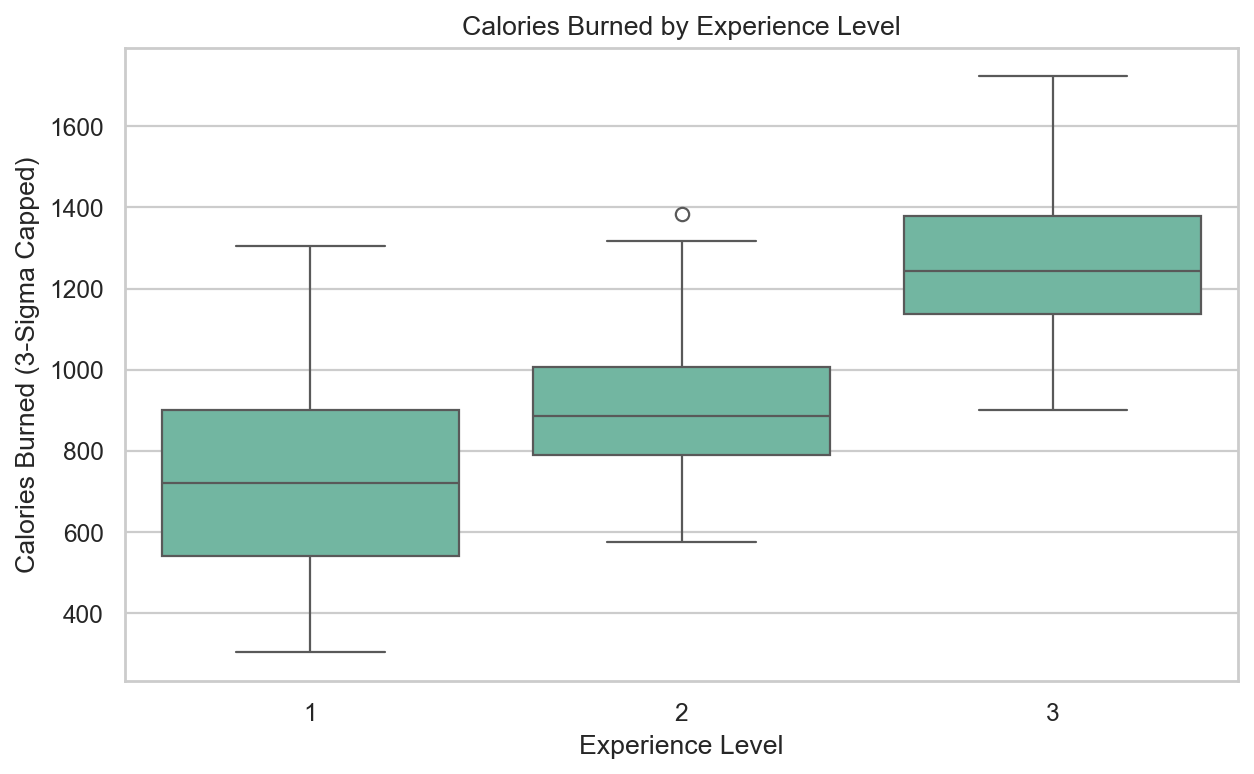
\includegraphics[width=0.86\linewidth]{../docs/figures/week1/calories_by_experience_level.png}
    \caption{EDA: calories burned by experience level.}
\end{figure}

\begin{figure}[H]
    \centering
    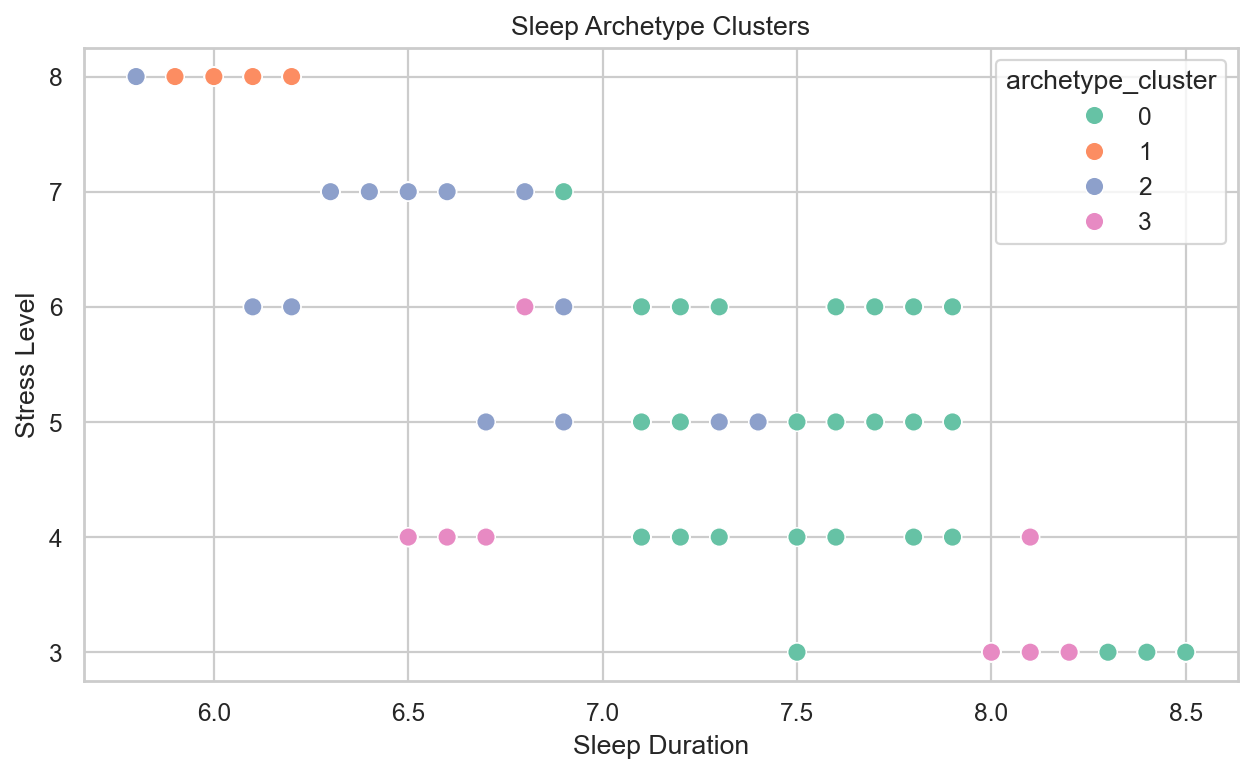
\includegraphics[width=0.86\linewidth]{../docs/figures/week1/sleep_archetype_clusters.png}
    \caption{EDA: sleep archetype clusters.}
\end{figure}

\begin{figure}[H]
    \centering
    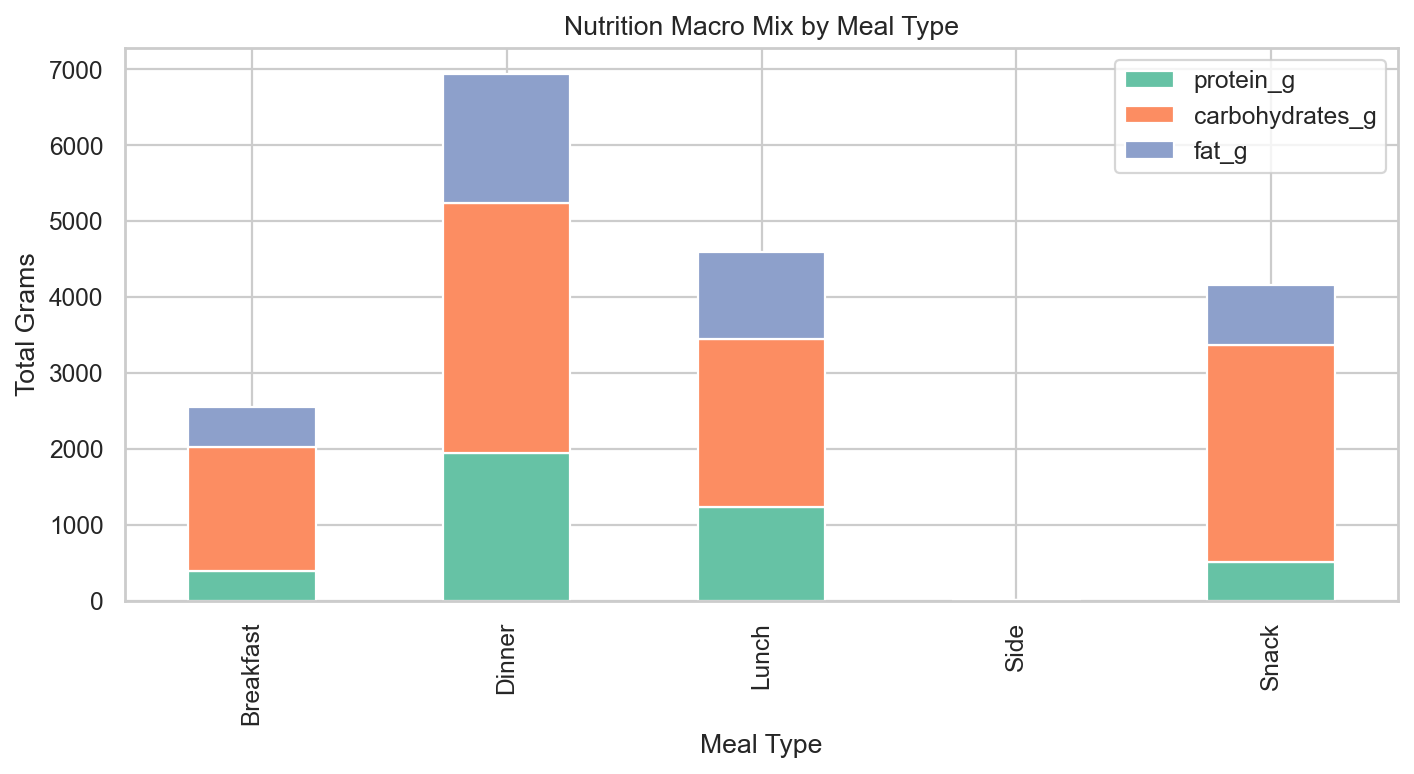
\includegraphics[width=0.86\linewidth]{../docs/figures/week1/nutrition_macro_mix_by_meal_type.png}
    \caption{EDA: nutrition macro mix by meal type.}
\end{figure}

\begin{figure}[H]
    \centering
    \begin{subfigure}[t]{0.48\linewidth}
        \centering
        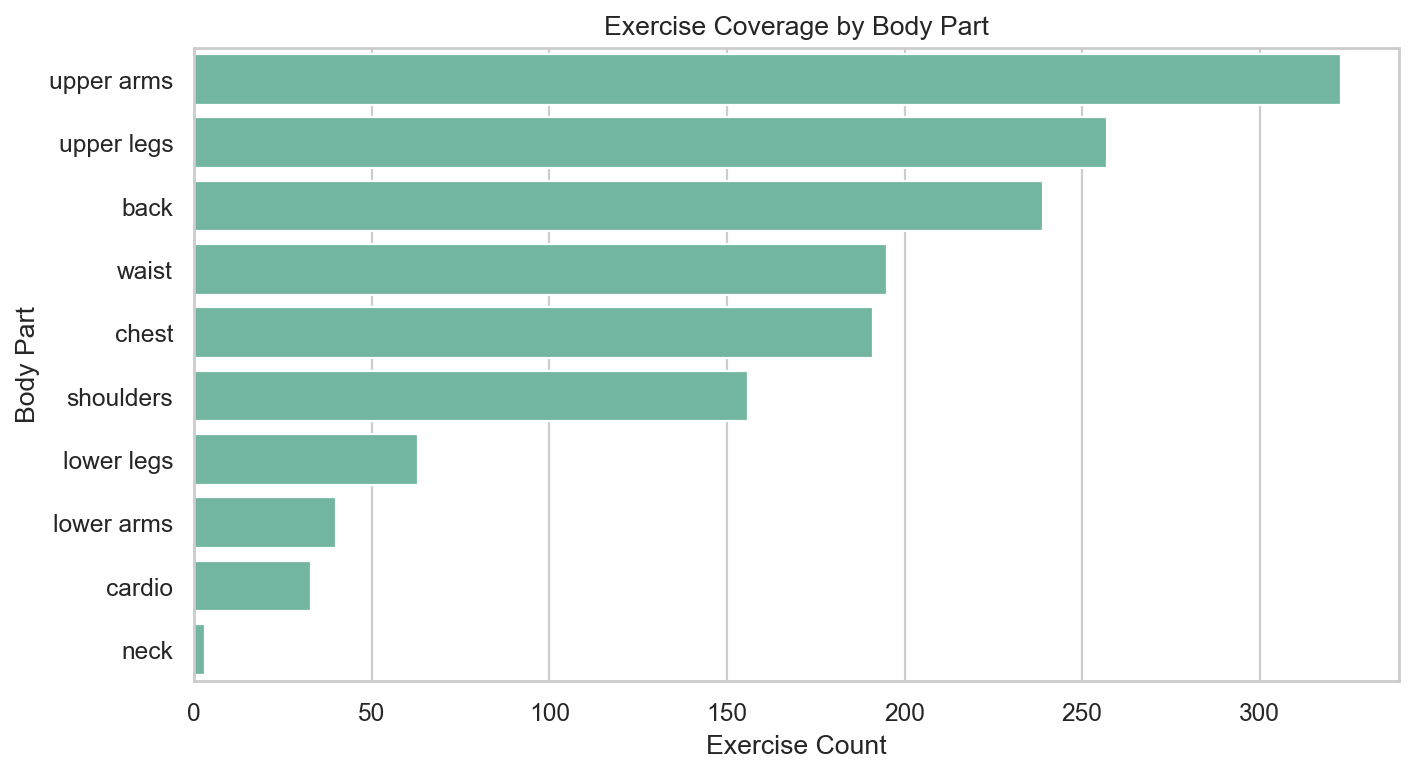
\includegraphics[width=\linewidth]{../docs/figures/week1/exercise_coverage_by_body_part.png}
        \caption{Body-part coverage}
    \end{subfigure}
    \hfill
    \begin{subfigure}[t]{0.48\linewidth}
        \centering
        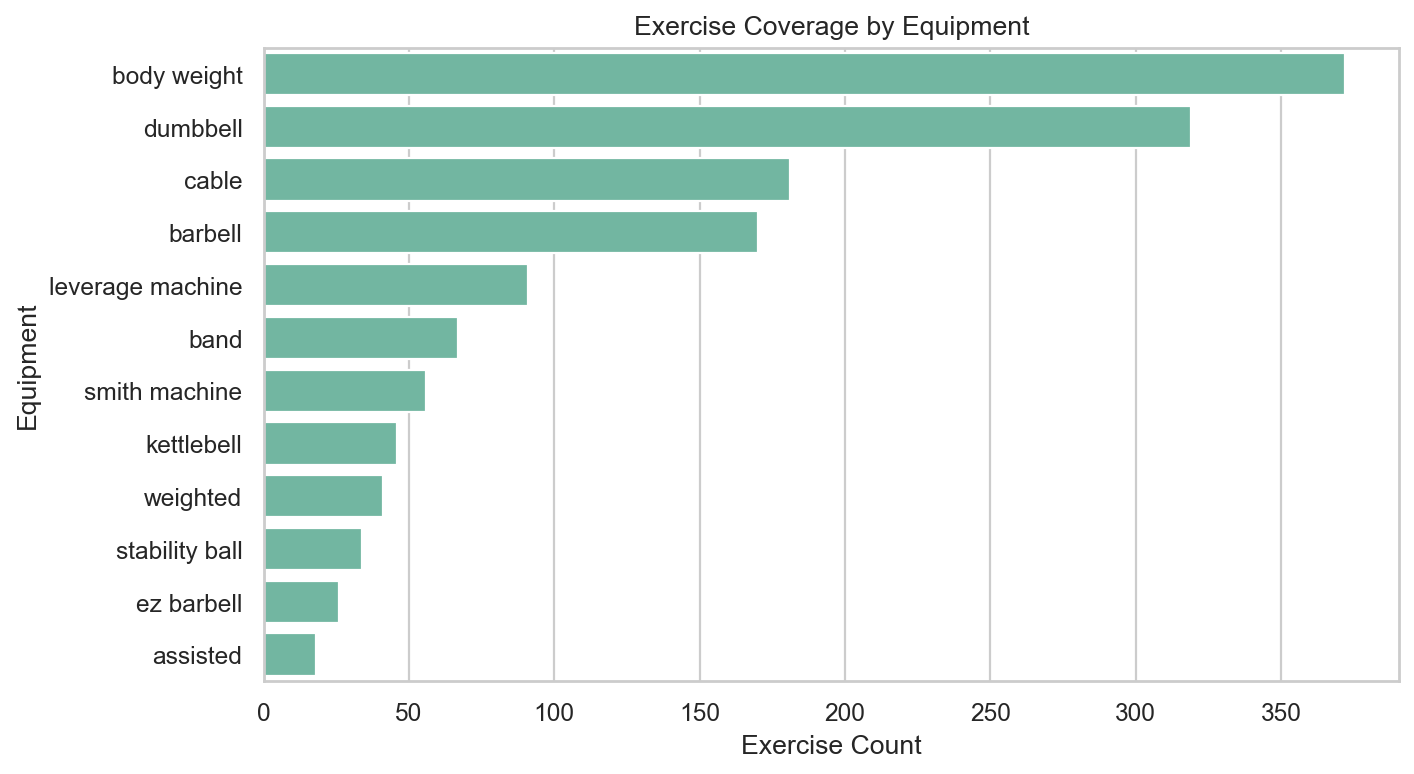
\includegraphics[width=\linewidth]{../docs/figures/week1/exercise_coverage_by_equipment.png}
        \caption{Equipment coverage}
    \end{subfigure}
    \caption{EDA: ExerciseDB coverage for RAG retrieval.}
\end{figure}

\begin{figure}[H]
    \centering
    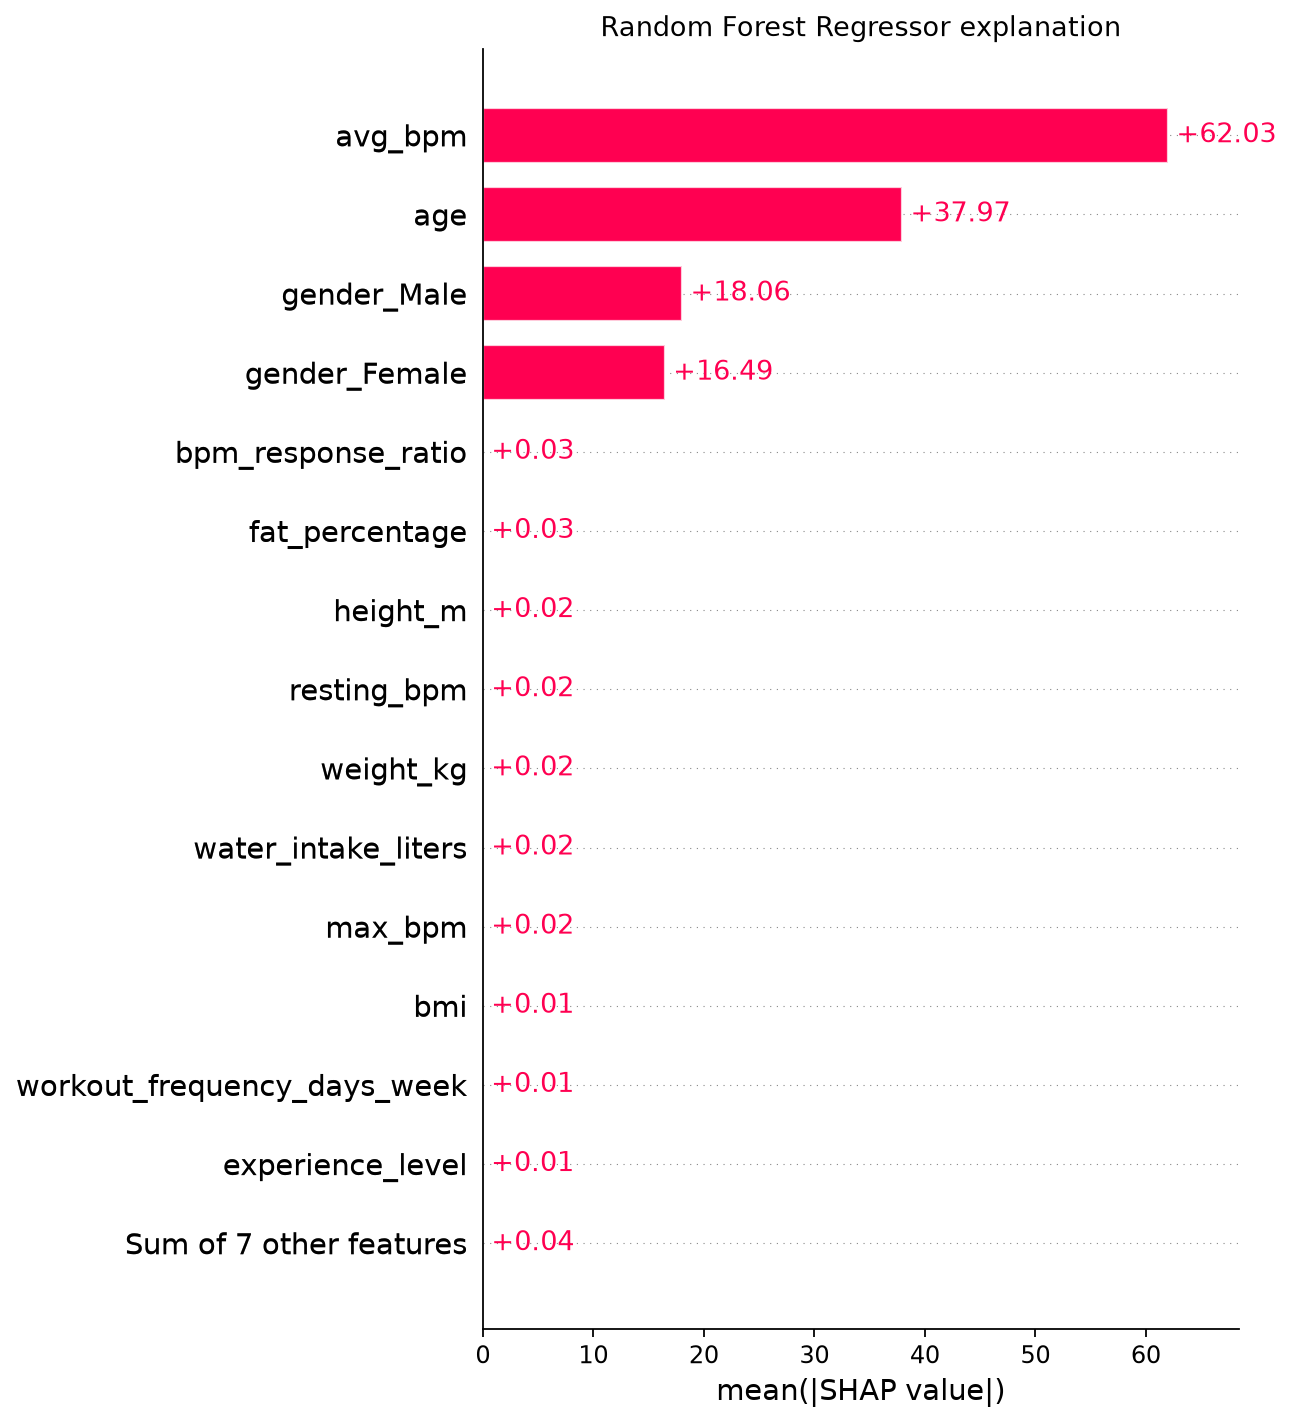
\includegraphics[width=0.86\linewidth]{../docs/figures/week2/selected_calorie_regressor_shap.png}
    \caption{SHAP explanation: calorie-burn-rate regressor.}
    
    \label{fig:appendix_calorie_shap}
\end{figure}

\begin{figure}[H]
    \centering
    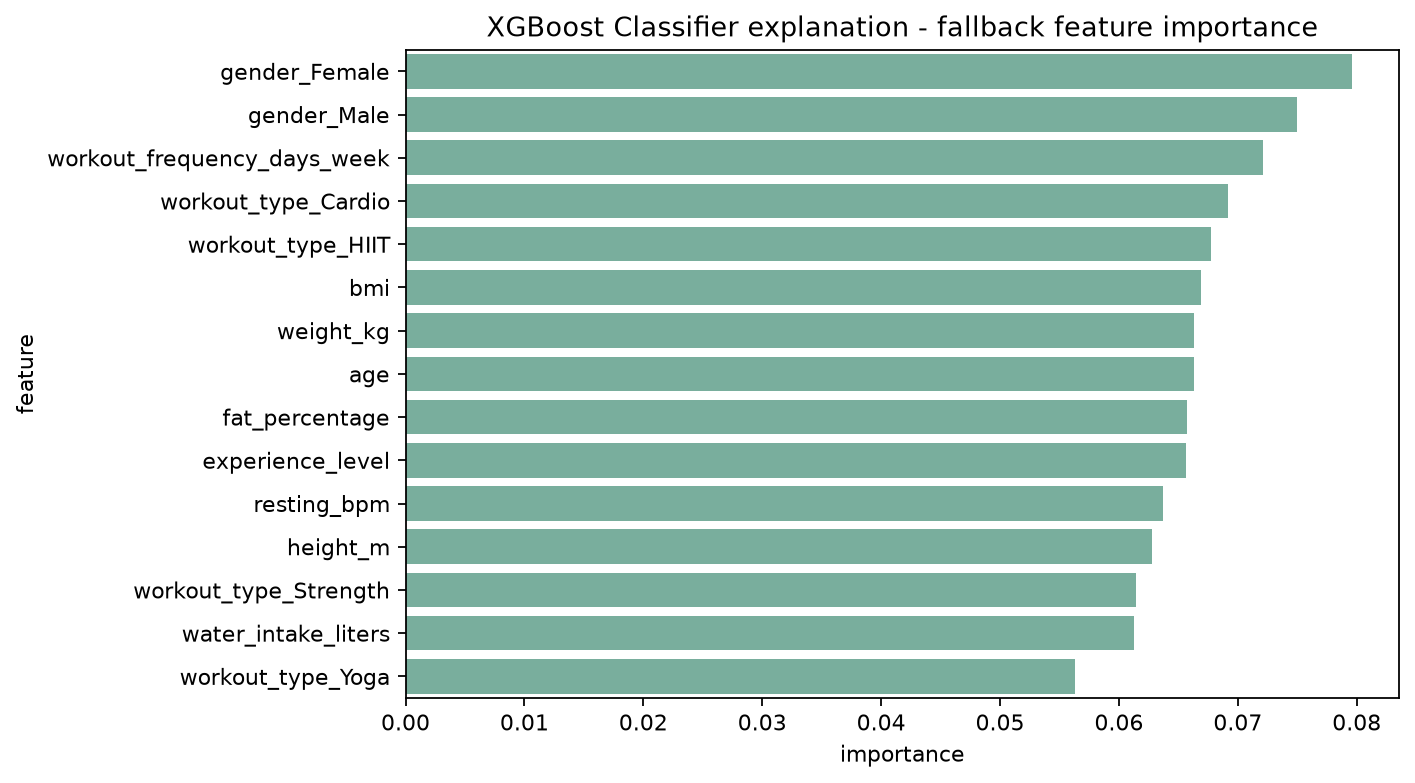
\includegraphics[width=0.86\linewidth]{../docs/figures/week2/selected_intensity_classifier_shap.png}
    \caption{SHAP explanation: intensity classifier.}
\end{figure}

\begin{figure}[H]
    \centering
    \begin{subfigure}[t]{0.47\linewidth}
        \centering
        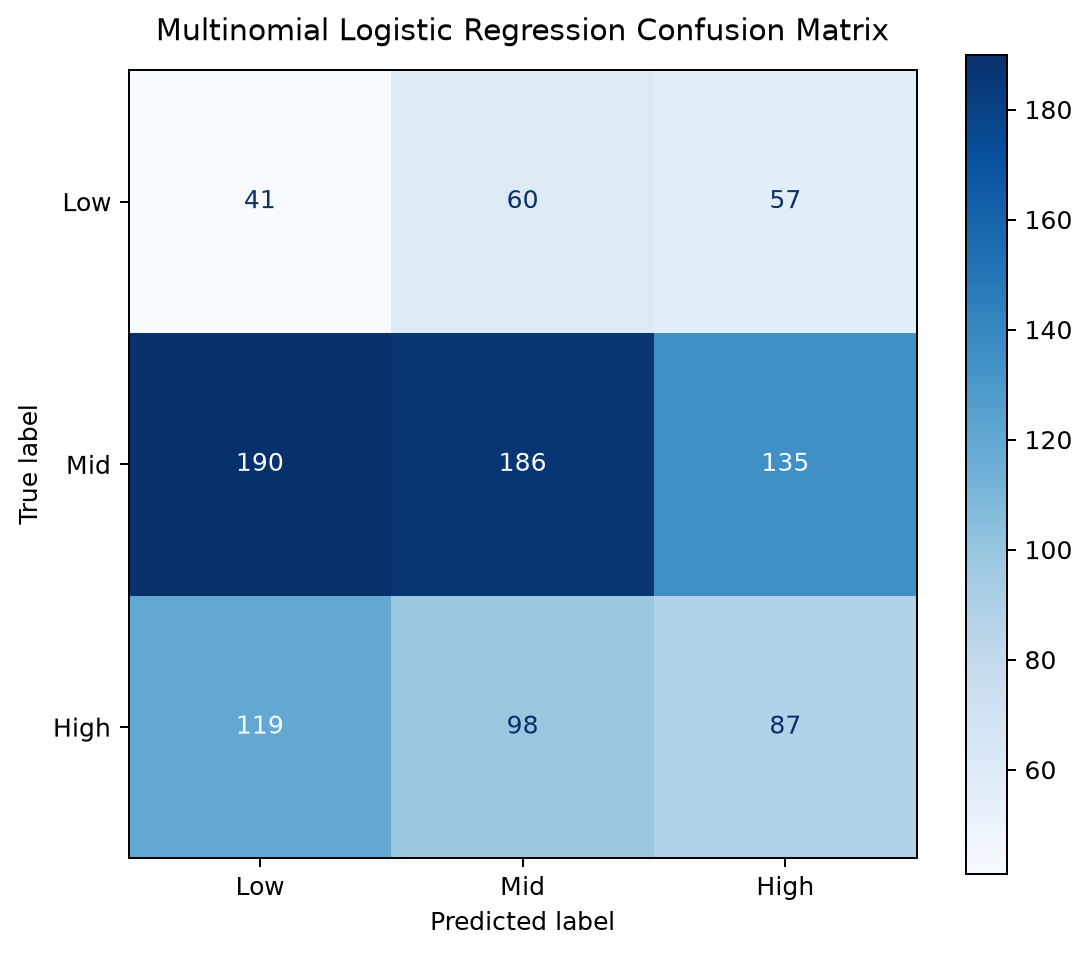
\includegraphics[width=\linewidth]{../docs/figures/week2/multinomial_logistic_regression_confusion_matrix.png}
        \caption{Logistic Regression}
    \end{subfigure}
    \hfill
    \begin{subfigure}[t]{0.47\linewidth}
        \centering
        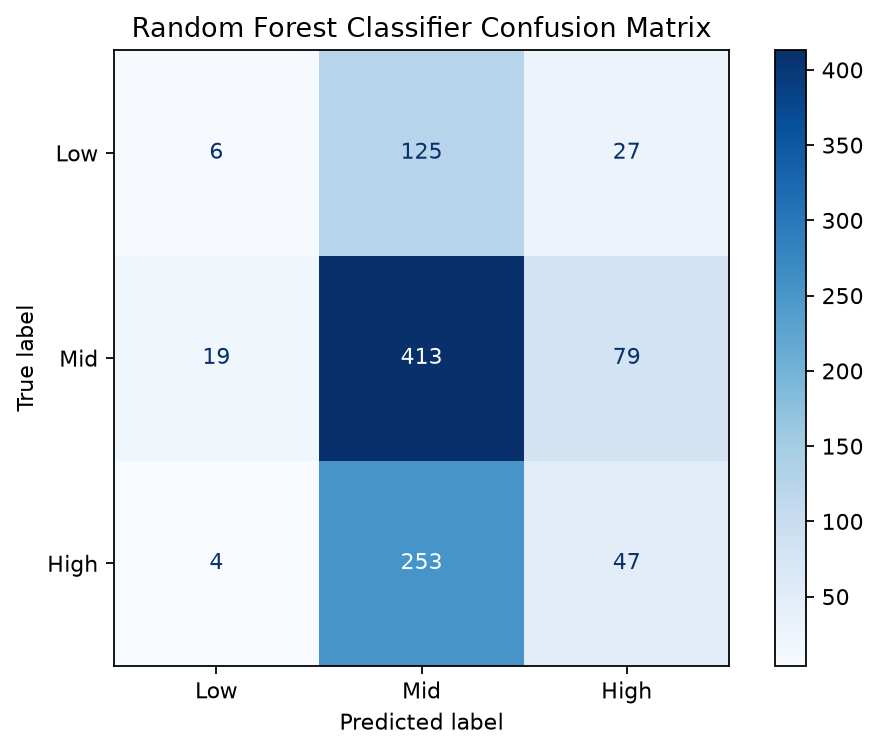
\includegraphics[width=\linewidth]{../docs/figures/week2/random_forest_classifier_confusion_matrix.png}
        \caption{Random Forest}
    \end{subfigure}\\[3pt]
    \begin{subfigure}[t]{0.47\linewidth}
        \centering
        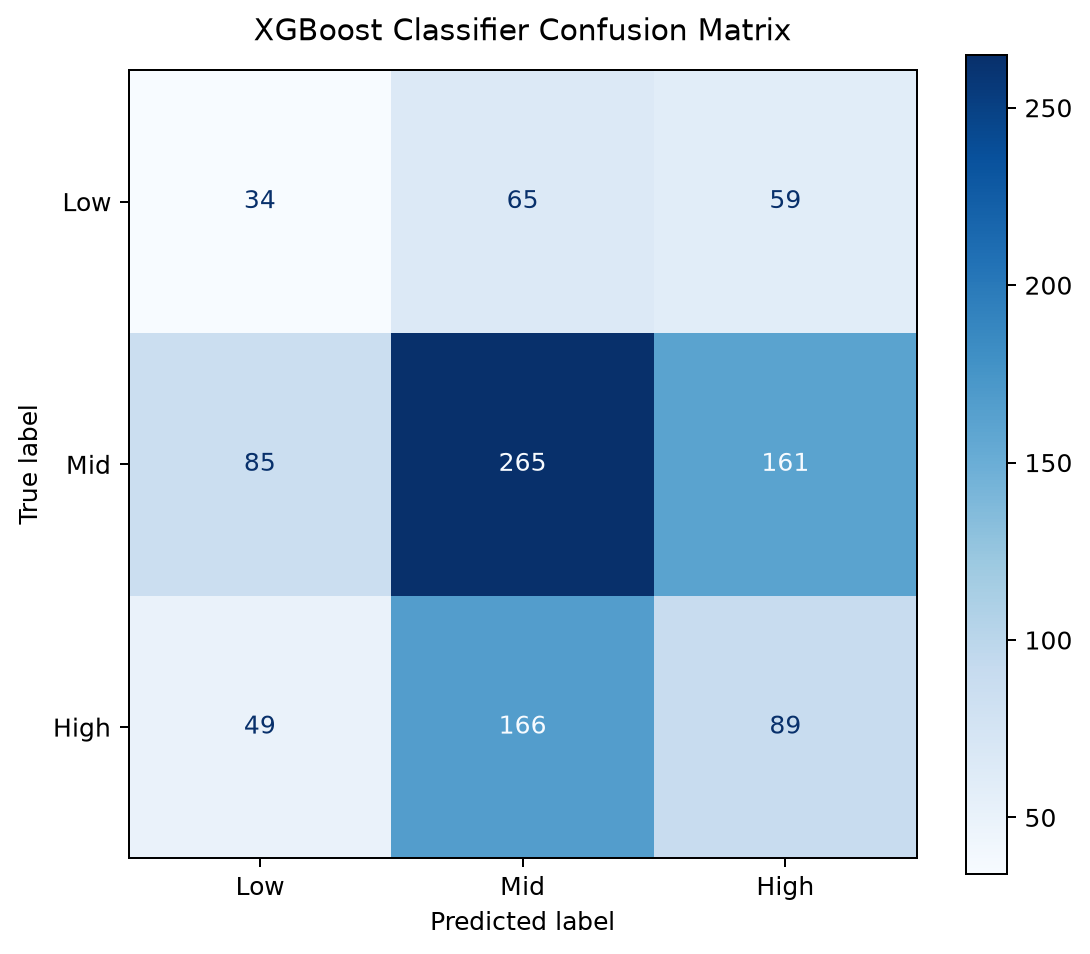
\includegraphics[width=\linewidth]{../docs/figures/week2/xgboost_classifier_confusion_matrix.png}
        \caption{XGBoost}
    \end{subfigure}
    \caption{Classifier confusion matrices: Low/Mid/High intensity.}
    \label{fig:confusematrix}
\end{figure}
\end{document}

